\begin{enumerate}[label=\thesection.\arabic*,ref=\thesection.\theenumi]
\numberwithin{equation}{enumi}
\numberwithin{figure}{enumi}
\numberwithin{table}{enumi}
\item 
\label{chapters/9/10/4/1}
\iffalse
\documentclass[journal,12pt,twocolumn]{article}
\usepackage{graphicx}
\usepackage[none]{hyphenat}
\usepackage[margin=0.5in]{geometry}
\usepackage[cmex10]{amsmath}
\usepackage{array}
\usepackage{booktabs}
\usepackage{gensymb}
\usepackage{textcomp}
\title{\textbf{circle Assignment}}
\author{Dulla Srinivas - FWC22041}
\date{\today}
\providecommand{\norm}[1]{\left\lVert#1\right\rVert}
\providecommand{\abs}[1]{\left\vert#1\right\vert}
\let\vec\mathbf
\newcommand{\myvec}[1]{\ensuremath{\begin{pmatrix}#1\end{pmatrix}}}
\newcommand{\mydet}[1]{\ensuremath{\begin{vmatrix}#1\end{vmatrix}}}
\providecommand{\brak}[1]{\ensuremath{\left(#1\right)}}

\begin{document}

\maketitle
\section*{Problem Statement:}
\fi
Two circles of radii 5cm and 3cm intersect at two points and the distance between their center is 4cm. Find the length of the common chord.
\\
\solution 
See Fig. 
		\ref{fig:9/10/4/1}.
		and
	\begin{figure}[!h]
		\centering
 \includegraphics[width=\columnwidth]{chapters/9/10/4/1/figs/cccc.png}
		\caption{}
		\label{fig:9/10/4/1}
  	\end{figure}

	\begin{table}[!h]
		\centering
 %%%%%%%%%%%%%%%%%%%%%%%%%%%%%%%%%%%%%%%%%%%%%%%%%%%%%%%%%%%%%%%%%%%%%%
%%                                                                  %%
%%  This is the header of a LaTeX2e file exported from Gnumeric.    %%
%%                                                                  %%
%%  This file can be compiled as it stands or included in another   %%
%%  LaTeX document. The table is based on the longtable package so  %%
%%  the longtable options (headers, footers...) can be set in the   %%
%%  preamble section below (see PRAMBLE).                           %%
%%                                                                  %%
%%  To include the file in another, the following two lines must be %%
%%  in the including file:                                          %%
%%        \def\inputGnumericTable{}                                 %%
%%  at the beginning of the file and:                               %%
%%        \input{name-of-this-file.tex}                             %%
%%  where the table is to be placed. Note also that the including   %%
%%  file must use the following packages for the table to be        %%
%%  rendered correctly:                                             %%
%%    \usepackage[latin1]{inputenc}                                 %%
%%    \usepackage{color}                                            %%
%%    \usepackage{array}                                            %%
%%    \usepackage{longtable}                                        %%
%%    \usepackage{calc}                                             %%
%%    \usepackage{multirow}                                         %%
%%    \usepackage{hhline}                                           %%
%%    \usepackage{ifthen}                                           %%
%%  optionally (for landscape tables embedded in another document): %%
%%    \usepackage{lscape}                                           %%
%%                                                                  %%
%%%%%%%%%%%%%%%%%%%%%%%%%%%%%%%%%%%%%%%%%%%%%%%%%%%%%%%%%%%%%%%%%%%%%%



%%  This section checks if we are begin input into another file or  %%
%%  the file will be compiled alone. First use a macro taken from   %%
%%  the TeXbook ex 7.7 (suggestion of Han-Wen Nienhuys).            %%
\def\ifundefined#1{\expandafter\ifx\csname#1\endcsname\relax}


%%  Check for the \def token for inputed files. If it is not        %%
%%  defined, the file will be processed as a standalone and the     %%
%%  preamble will be used.                                          %%
\ifundefined{inputGnumericTable}

%%  We must be able to close or not the document at the end.        %%
	\def\gnumericTableEnd{\end{document}}


%%%%%%%%%%%%%%%%%%%%%%%%%%%%%%%%%%%%%%%%%%%%%%%%%%%%%%%%%%%%%%%%%%%%%%
%%                                                                  %%
%%  This is the PREAMBLE. Change these values to get the right      %%
%%  paper size and other niceties.                                  %%
%%                                                                  %%
%%%%%%%%%%%%%%%%%%%%%%%%%%%%%%%%%%%%%%%%%%%%%%%%%%%%%%%%%%%%%%%%%%%%%%

	\documentclass[12pt%
			  %,landscape%
                    ]{report}
       \usepackage[latin1]{inputenc}
       \usepackage{fullpage}
       \usepackage{color}
       \usepackage{array}
       \usepackage{longtable}
       \usepackage{calc}
       \usepackage{multirow}
       \usepackage{hhline}
       \usepackage{ifthen}

	\begin{document}


%%  End of the preamble for the standalone. The next section is for %%
%%  documents which are included into other LaTeX2e files.          %%
\else

%%  We are not a stand alone document. For a regular table, we will %%
%%  have no preamble and only define the closing to mean nothing.   %%
    \def\gnumericTableEnd{}

%%  If we want landscape mode in an embedded document, comment out  %%
%%  the line above and uncomment the two below. The table will      %%
%%  begin on a new page and run in landscape mode.                  %%
%       \def\gnumericTableEnd{\end{landscape}}
%       \begin{landscape}


%%  End of the else clause for this file being \input.              %%
\fi

%%%%%%%%%%%%%%%%%%%%%%%%%%%%%%%%%%%%%%%%%%%%%%%%%%%%%%%%%%%%%%%%%%%%%%
%%                                                                  %%
%%  The rest is the gnumeric table, except for the closing          %%
%%  statement. Changes below will alter the table's appearance.     %%
%%                                                                  %%
%%%%%%%%%%%%%%%%%%%%%%%%%%%%%%%%%%%%%%%%%%%%%%%%%%%%%%%%%%%%%%%%%%%%%%

\providecommand{\gnumericmathit}[1]{#1} 
%%  Uncomment the next line if you would like your numbers to be in %%
%%  italics if they are italizised in the gnumeric table.           %%
%\renewcommand{\gnumericmathit}[1]{\mathit{#1}}
\providecommand{\gnumericPB}[1]%
{\let\gnumericTemp=\\#1\let\\=\gnumericTemp\hspace{0pt}}
 \ifundefined{gnumericTableWidthDefined}
        \newlength{\gnumericTableWidth}
        \newlength{\gnumericTableWidthComplete}
        \newlength{\gnumericMultiRowLength}
        \global\def\gnumericTableWidthDefined{}
 \fi
%% The following setting protects this code from babel shorthands.  %%
 \ifthenelse{\isundefined{\languageshorthands}}{}{\languageshorthands{english}}
%%  The default table format retains the relative column widths of  %%
%%  gnumeric. They can easily be changed to c, r or l. In that case %%
%%  you may want to comment out the next line and uncomment the one %%
%%  thereafter                                                      %%
\providecommand\gnumbox{\makebox[0pt]}
%%\providecommand\gnumbox[1][]{\makebox}

%% to adjust positions in multirow situations                       %%
\setlength{\bigstrutjot}{\jot}
\setlength{\extrarowheight}{\doublerulesep}

%%  The \setlongtables command keeps column widths the same across  %%
%%  pages. Simply comment out next line for varying column widths.  %%
\setlongtables

\setlength\gnumericTableWidth{%
	55pt+%
	32pt+%
	86pt+%
	70pt+%
0pt}
\def\gumericNumCols{4}
\setlength\gnumericTableWidthComplete{\gnumericTableWidth+%
         \tabcolsep*\gumericNumCols*2+\arrayrulewidth*\gumericNumCols}
\ifthenelse{\lengthtest{\gnumericTableWidthComplete > \linewidth}}%
         {\def\gnumericScale{1*\ratio{\linewidth-%
                        \tabcolsep*\gumericNumCols*2-%
                        \arrayrulewidth*\gumericNumCols}%
{\gnumericTableWidth}}}%
{\def\gnumericScale{1}}

%%%%%%%%%%%%%%%%%%%%%%%%%%%%%%%%%%%%%%%%%%%%%%%%%%%%%%%%%%%%%%%%%%%%%%
%%                                                                  %%
%% The following are the widths of the various columns. We are      %%
%% defining them here because then they are easier to change.       %%
%% Depending on the cell formats we may use them more than once.    %%
%%                                                                  %%
%%%%%%%%%%%%%%%%%%%%%%%%%%%%%%%%%%%%%%%%%%%%%%%%%%%%%%%%%%%%%%%%%%%%%%

\ifthenelse{\isundefined{\gnumericColA}}{\newlength{\gnumericColA}}{}\settowidth{\gnumericColA}{\begin{tabular}{@{}p{55pt*\gnumericScale}@{}}x\end{tabular}}
\ifthenelse{\isundefined{\gnumericColB}}{\newlength{\gnumericColB}}{}\settowidth{\gnumericColB}{\begin{tabular}{@{}p{32pt*\gnumericScale}@{}}x\end{tabular}}
\ifthenelse{\isundefined{\gnumericColC}}{\newlength{\gnumericColC}}{}\settowidth{\gnumericColC}{\begin{tabular}{@{}p{86pt*\gnumericScale}@{}}x\end{tabular}}
\ifthenelse{\isundefined{\gnumericColD}}{\newlength{\gnumericColD}}{}\settowidth{\gnumericColD}{\begin{tabular}{@{}p{70pt*\gnumericScale}@{}}x\end{tabular}}

\begin{longtable}[c]{%
	b{\gnumericColA}%
	b{\gnumericColB}%
	b{\gnumericColC}%
	b{\gnumericColD}%
	}

%%%%%%%%%%%%%%%%%%%%%%%%%%%%%%%%%%%%%%%%%%%%%%%%%%%%%%%%%%%%%%%%%%%%%%
%%  The longtable options. (Caption, headers... see Goosens, p.124) %%
%	\caption{The Table Caption.}             \\	%
% \hline	% Across the top of the table.
%%  The rest of these options are table rows which are placed on    %%
%%  the first, last or every page. Use \multicolumn if you want.    %%

%%  Header for the first page.                                      %%
%	\multicolumn{4}{c}{The First Header} \\ \hline 
%	\multicolumn{1}{c}{colTag}	%Column 1
%	&\multicolumn{1}{c}{colTag}	%Column 2
%	&\multicolumn{1}{c}{colTag}	%Column 3
%	&\multicolumn{1}{c}{colTag}	\\ \hline %Last column
%	\endfirsthead

%%  The running header definition.                                  %%
%	\hline
%	\multicolumn{4}{l}{\ldots\small\slshape continued} \\ \hline
%	\multicolumn{1}{c}{colTag}	%Column 1
%	&\multicolumn{1}{c}{colTag}	%Column 2
%	&\multicolumn{1}{c}{colTag}	%Column 3
%	&\multicolumn{1}{c}{colTag}	\\ \hline %Last column
%	\endhead

%%  The running footer definition.                                  %%
%	\hline
%	\multicolumn{4}{r}{\small\slshape continued\ldots} \\
%	\endfoot

%%  The ending footer definition.                                   %%
%	\multicolumn{4}{c}{That's all folks} \\ \hline 
%	\endlastfoot
%%%%%%%%%%%%%%%%%%%%%%%%%%%%%%%%%%%%%%%%%%%%%%%%%%%%%%%%%%%%%%%%%%%%%%

\hhline{|-|-|-~}
	 \multicolumn{1}{|p{\gnumericColA}|}%
	{\gnumericPB{\centering}\gnumbox{\textbf{Parameter}}}
	&\multicolumn{1}{p{\gnumericColB}|}%
	{\gnumericPB{\centering}\gnumbox{\textbf{Value}}}
	&\multicolumn{1}{p{\gnumericColC}|}%
	{\gnumericPB{\centering}\gnumbox{\textbf{Description}}}
	&
\\
\hhline{|---|~}
	 \multicolumn{1}{|p{\gnumericColA}|}%
	{\gnumericPB{\centering}\gnumbox{$\vec{c}_1$}}
	&\multicolumn{1}{p{\gnumericColB}|}%
	{\gnumericPB{\centering}\gnumbox{$\vec{0}$}}
	&\multicolumn{1}{p{\gnumericColC}|}%
	{\gnumericPB{\centering}\gnumbox{Center of Circle 1}}
	&
\\
\hhline{|---|~}
	 \multicolumn{1}{|p{\gnumericColA}|}%
	{\gnumericPB{\centering}\gnumbox{$\vec{c}_2$}}
	&\multicolumn{1}{p{\gnumericColB}|}%
	{\gnumericPB{\centering}\gnumbox{$4\vec{e}_1$}}
	&\multicolumn{1}{p{\gnumericColC}|}%
	{\gnumericPB{\centering}\gnumbox{Center of Circle 2}}
	&
\\
\hhline{|---|~}
	 \multicolumn{1}{|p{\gnumericColA}|}%
	{\gnumericPB{\centering}\gnumbox{$r_1$}}
	&\multicolumn{1}{p{\gnumericColB}|}%
	{\gnumericPB{\centering}\gnumbox{5}}
	&\multicolumn{1}{p{\gnumericColC}|}%
	{\gnumericPB{\centering}\gnumbox{Radius of Circle 1}}
	&
\\
\hhline{|---|~}
	 \multicolumn{1}{|p{\gnumericColA}|}%
	{\gnumericPB{\centering}\gnumbox{$r_2$}}
	&\multicolumn{1}{p{\gnumericColB}|}%
	{\gnumericPB{\centering}\gnumbox{3}}
	&\multicolumn{1}{p{\gnumericColC}|}%
	{\gnumericPB{\centering}\gnumbox{Radius of Circle 2}}
	&
\\
\hhline{|-|-|-|~}
\end{longtable}

\ifthenelse{\isundefined{\languageshorthands}}{}{\languageshorthands{\languagename}}
\gnumericTableEnd

		\caption{}
		\label{tab:9/10/4/1}
  	\end{table}
	From 
		Table 
		\ref{tab:9/10/4/1},
	\eqref{eq:circ-eq}
	and
	\eqref{eq:circ-cr},
	the equations of the two circles are
\begin{align}
	\begin{split}
	\norm{\vec{x}}^2 -25 &= 0
	\\
	\norm{\vec{x}}^2 - 8 \vec{e}_1^{\top}\vec{x} +7 &= 0
	\end{split}
		\label{eq:9/10/4/1/circs}
\end{align}
From 
		\eqref{eq:9/10/4/1/circs}
and
	\eqref{eq:circ-chord}
the equation of the common chord is 
\begin{align}
	   \vec{e}_1^{\top}\vec{x} 
	   &= 4
		\label{eq:9/10/4/1/chord}
\end{align}
%
It is easy to verify that 
\begin{align}
	\vec{q} = 4\vec{e}_1
\end{align}
is a point on 
		\eqref{eq:9/10/4/1/chord}.
		Substituting
\begin{align}
\vec{m} = \vec{e}_2, \vec{q} = 4\vec{e}_1, 
\vec{V}=\vec{I}, \vec{u} = \vec{0}, f = -25
\end{align}
in 
\eqref{eq:chord-len},
		the length of the chord in 
\eqref{eq:conic_tangent}
is given by 
\begin{align}
 \frac{2\sqrt{
\sbrak{
\vec{e}_2^{\top}\brak{4\vec{e}_1}
}^2
-
\brak
{
16\vec{e}_1^{\top}\vec{e}_1 -25
}
\brak{\vec{e}_2^{\top}\vec{e}_2}
}
}
{
\vec{e}_2^{\top}\vec{e}_2
}\norm{\vec{e}_2}
= 6
  \end{align}
	

\iffalse

/sdcard/github/matrix-analysis/chapters/9/10/4/1/tables/table-9-10-4-1.tex
\section*{Solution:}

\begin{figure}[h]
\centering
\includegraphics[width=\columnwidth]{cccc.png}
\caption{Diagram generated using python}
\label{fig:square}
\end{figure}
\subsection{Theory:}
{They given two circles radius first circle radii is 5cm(Q1) and  second circle radii is 3cm(Q2) distance between circle 1 and circle 2 is 4cm. we have find the length of the chord.  }

\subsection{Mathematical Calculation:}
$\vec{O} = \myvec{0\\0}$ 
\end{center}
\subsection{Deriving equation for Circle in matrix form}
\vspace{0.2cm}
\begin{flushleft}
The equation of circle in matrix form is,\\
\vspace{0.25cm}
\end{flushleft}
\vspace{0.25cm}
\begin{equation}
 \vec{x}^T \vec{V} \vec{x} + 2 \vec{u}^T \vec{x} + f = 0
\end{equation}
\begin{flushleft}
Where\\
\end{flushleft}
\center
$\vec{V} = \vec{I}= \myvec{ 1 & 0\\ 0 & 1} , \vec{u} = \myvec{0 \\ 0}, \vec{f}=-25$\\
\endcenter
\center
  $\implies$  $ \vec{x}^T$$\vec{I}$ $\vec{x}$  + 2 $ \myvec{0\\0}^T \vec{x} -25 = 0$
\endcenter
\begin{flushleft}
\vspace{0.23cm}
Therefore, the circle equation can be written as
\end{flushleft}
\begin{equation}
    \vec{x}^T \vec{x} + 2 \myvec{0\\0}^T \vec{x} -25= 0
\end{equation}
\endcenter
\begin{flushleft}
The equation of circle in matrix form is,\\
\vspace{0.25cm}
\end{flushleft}
\vspace{0.25cm}
\begin{equation}
 \vec{x}^T \vec{V} \vec{x} + 2 \vec{u}^T \vec{x} + f = 0
\end{equation}
\begin{flushleft}
Where\\
\end{flushleft}
\center
$\vec{V} = \vec{I}= \myvec{ 1 & 0\\ 0 & 1} , \vec{u} = \myvec{-4 \\ 0}, \vec{f}=7$\\  \vspace{10mm}
\endcenter
\center
  $\implies$  $ \vec{x}^T$$\vec{I}$ $\vec{x}$  + 2 $ \myvec{-4\\0}^T \vec{x} +7= 0$
\endcenter
\begin{flushleft}
\vspace{0.23cm}
Therefore, the circle equation can be written as
\begin{equation}
    \vec{x}^T \vec{x} + 2 \myvec{-4\\0}^T \vec{x} +7= 0
\end{equation}

  Here we have to Find the Intersection of Two conics
\begin{equation}
 \vec{x}^T \vec{V_1} \vec{x} + 2 \vec{u_1}^T \vec{x} + \vec f_1 = 0
\end{equation}




\begin{equation} 
\vec{x}^T \vec{V_2} \vec{x} + 2 \vec{u_2}^T \vec{x} + \vec f_2 = 0
\end{equation}
The locus of their pair of straight lines\\

\begin{equation}                       
	\vec{x}^T \vec{(V_1+\mu V_2)x}+2\vec{(u_1+\mu u_2)x}^T \vec x + \vec f_1+ \vec f_2  = 0              
\end{equation}

  \begin{align}
\mydet{
\vec{V}_1+ \mu \vec{V}_2&\vec{u}_1+\mu\vec{u}_2
\\
	\brak{\vec{u}_1+\mu\vec{u}_2}^{\top}&f_1 +f_2
}
	= 0, 
%    \label{eq:conic_quad_form_int-mat}
\end{align}

 

\begin{align}
	\vec {V_1} = \myvec{  1 \hspace{10mm} 0  \vspace{4mm} \hspace{10mm }\\ 0  \hspace{10mm} 1 \\ } \\  \vspace{5mm}
\vec {V_2} = \myvec{  1 \hspace{10mm} 0  \vspace{4mm} \hspace{10mm }\\ 0  \hspace{10mm} 1\\ } \\ \vspace{5mm}
\vec {u_1} = \myvec{  0    \vspace{4mm} \hspace{10mm }\\ 0 \hspace{10mm} \\ } \\ \vspace{5mm}
\vec {u_2} = \myvec{  -4   \vspace{4mm} \hspace{10mm }\\ 0 \hspace{10mm} \\ } \\ \vspace{5mm}
\vec f_1=-25  \hspace{10mm}
\vec f_2=7
\vspace{5mm}
 = \myvec{I +\mu I\hspace{10mm} 0- \myvec{4 \\ 0},  \vspace{4mm}\\ 0-\mu (4,0) \hspace{10mm} 0\\      }\\
\vspace{10mm}
= \myvec{1 +\mu \hspace{10mm} 0 \hspace{10mm}  \myvec{-4\mu},  \vspace{4mm}\\ 0  \hspace{10mm} 1+\mu \hspace{10mm} 0  ,\vspace{4mm}\\ -4 \mu  \hspace{10mm} 0  \hspace{10mm} 7\mu - 25 \\      }\\
\vspace{10mm}
= \myvec{-25 \mu + 7\mu +\mu \hspace{10mm} -16\mu^2\hspace{10mm}  ,  \vspace{4mm}\\ 0  \hspace{20mm} -25\mu + 7\mu+\mu  ,\vspace{4mm}\\ }\\
\vspace{10mm}
\mu = -1
\vspace{10mm}
\end{align}

 
 
 \subsection{According to the equation 7}
 2\myvec{-1 \myvec{-4\\0} x }-25-7=0\\
 \vspace{5mm}
 
\vspace{5mm}
  8x = 32\\
  \vspace{5mm}
   x=4\\
    \vspace{5mm}
    
    So,  = \myvec{4\\ 3} - \myvec{4 \\ -3}
    \hspace{5mm}
 $   p_1=(4,-3)$
\subsection{ So The length of the common chord is 6cm}
   $$= || p - p_1|| $$
        = \myvec{4\\ 3} - \myvec{4 \\ -3} \\
        \vspace{5mm}
        =6
  \section*{\large Construction}
{
\setlength\extrarowheight{5pt}
\begin{tabular}{|c|c|c|}
  \hline
  \textbf{Symbol}&\textbf{Value}&\textbf{Description}\\
  \hline
	$r_1$&5&Radius \\
  \hline
	$r_2$&3&Radius\\
  \hline
  O&$(0,0)$&Center\\
  \hline
  O_1& $(4,0)$ &Center\\
  \hline
  P&$(4,3)$&Point Of intersection\\
  \hline
  P_1&$(4,-3)$&Point Of intersection\\
  \hline
  P-P_1& $6$ &Length of the common chord\\
  \hline
  
  
\end{tabular}
}
\end{document}
\fi

\item If two equal chords of a circle intersect within the circle, prove 
that the segments of one chord are equal to corresponding segments of the other 
chord.
\label{chapters/9/10/4/2}
\\
\solution 
\iffalse
\documentclass[10pt]{article}
       \usepackage[latin1]{inputenc}
       \usepackage{fullpage}
       \usepackage{color}
       \usepackage{array}
       \usepackage{longtable}
       \usepackage{calc}
       \usepackage{multirow}
       \usepackage{hhline}
       \usepackage{ifthen}
\usepackage{graphicx}
\def\inputGnumericTable{}
\usepackage[none]{hyphenat}
\usepackage{graphicx}
\usepackage{listings}
\usepackage[english]{babel}
\usepackage{graphicx}
\usepackage{caption} 
\usepackage{booktabs}
\usepackage{gensymb}
\usepackage{array}
\usepackage{amssymb} % for \because
\usepackage{amsmath}   % for having text in math mode
\usepackage{extarrows} % for Row operations arrows
\usepackage{listings}
\lstset{
  frame=single,
  breaklines=true
}
\usepackage{hyperref}
%Following 2 lines were added to remove the blank page at the beginning
\usepackage{atbegshi}% http://ctan.org/pkg/atbegshi
\AtBeginDocument{\AtBeginShipoutNext{\AtBeginShipoutDiscard}}
%New macro definitions
\newcommand{\mydet}[1]{\ensuremath{\begin{vmatrix}#1\end{vmatrix}}}
\providecommand{\brak}[1]{\ensuremath{\left(#1\right)}}
\providecommand{\norm}[1]{\left\lVert#1\right\rVert}
\newcommand{\solution}{\noindent \textbf{Solution: }}
\newcommand{\myvec}[1]{\ensuremath{\begin{pmatrix}#1\end{pmatrix}}}
\providecommand{\abs}[1]{\left\vert#1\right\vert}
\let\vec\mathbf
\begin{document}
\begin{center}
\title{\textbf{Properties of Circle}}
\date{\vspace{-5ex}} %Not to print date automatically
\maketitle
\end{center}
\setcounter{page}{1}
\section{9$^{th}$ Maths - Chapter 10}
       This is Problem-2 from Exercise 10.4
\begin{enumerate}
\item If two equal chords of a circle intersect within the circle, prove that the segments of one chord are equal to corresponding segments of other chord.

\solution:
\fi
\begin{figure}[h!]
	\begin{center} 
	  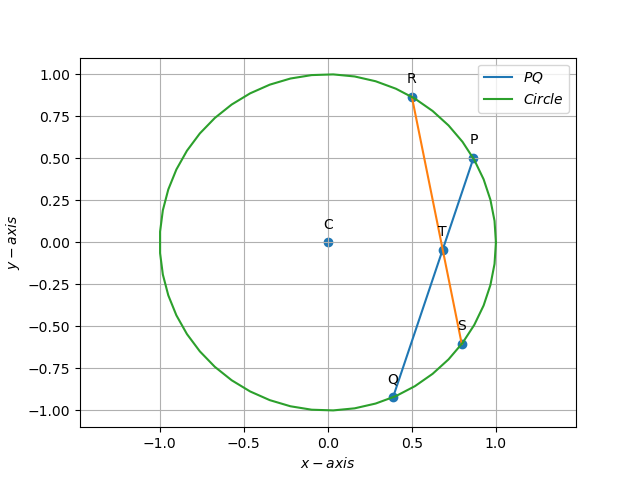
\includegraphics[width=\columnwidth]{chapters/9/10/4/2/figs/c.png}
	\end{center}
\caption{Two equal chords intersecting in a circle}
\label{fig:chapters/9/10/4/2/Fig1}
\end{figure} 
See Table 
\ref{tab:chapters/9/10/4/2/}
for the input  parameters.
\begin{table}[h!]
	%%%%%%%%%%%%%%%%%%%%%%%%%%%%%%%%%%%%%%%%%%%%%%%%%%%%%%%%%%%%%%%%%%%%%%
%%                                                                  %%
%%  This is the header of a LaTeX2e file exported from Gnumeric.    %%
%%                                                                  %%
%%  This file can be compiled as it stands or included in another   %%
%%  LaTeX document. The table is based on the longtable package so  %%
%%  the longtable options (headers, footers...) can be set in the   %%
%%  preamble section below (see PRAMBLE).                           %%
%%                                                                  %%
%%  To include the file in another, the following two lines must be %%
%%  in the including file:                                          %%
%%        \def\inputGnumericTable{}                                 %%
%%  at the beginning of the file and:                               %%
%%        \input{name-of-this-file.tex}                             %%
%%  where the table is to be placed. Note also that the including   %%
%%  file must use the following packages for the table to be        %%
%%  rendered correctly:                                             %%
%%    \usepackage[latin1]{inputenc}                                 %%
%%    \usepackage{color}                                            %%
%%    \usepackage{array}                                            %%
%%    \usepackage{longtable}                                        %%
%%    \usepackage{calc}                                             %%
%%    \usepackage{multirow}                                         %%
%%    \usepackage{hhline}                                           %%
%%    \usepackage{ifthen}                                           %%
%%  optionally (for landscape tables embedded in another document): %%
%%    \usepackage{lscape}                                           %%
%%                                                                  %%
%%%%%%%%%%%%%%%%%%%%%%%%%%%%%%%%%%%%%%%%%%%%%%%%%%%%%%%%%%%%%%%%%%%%%%



%%  This section checks if we are begin input into another file or  %%
%%  the file will be compiled alone. First use a macro taken from   %%
%%  the TeXbook ex 7.7 (suggestion of Han-Wen Nienhuys).            %%
\def\ifundefined#1{\expandafter\ifx\csname#1\endcsname\relax}


%%  Check for the \def token for inputed files. If it is not        %%
%%  defined, the file will be processed as a standalone and the     %%
%%  preamble will be used.                                          %%
\ifundefined{inputGnumericTable}

%%  We must be able to close or not the document at the end.        %%
	\def\gnumericTableEnd{\end{document}}


%%%%%%%%%%%%%%%%%%%%%%%%%%%%%%%%%%%%%%%%%%%%%%%%%%%%%%%%%%%%%%%%%%%%%%
%%                                                                  %%
%%  This is the PREAMBLE. Change these values to get the right      %%
%%  paper size and other niceties.                                  %%
%%                                                                  %%
%%%%%%%%%%%%%%%%%%%%%%%%%%%%%%%%%%%%%%%%%%%%%%%%%%%%%%%%%%%%%%%%%%%%%%

	\documentclass[12pt%
			  %,landscape%
                    ]{report}
       \usepackage[latin1]{inputenc}
       \usepackage{fullpage}
       \usepackage{color}
       \usepackage{array}
       \usepackage{longtable}
       \usepackage{calc}
       \usepackage{multirow}
       \usepackage{hhline}
       \usepackage{ifthen}

	\begin{document}


%%  End of the preamble for the standalone. The next section is for %%
%%  documents which are included into other LaTeX2e files.          %%
\else

%%  We are not a stand alone document. For a regular table, we will %%
%%  have no preamble and only define the closing to mean nothing.   %%
    \def\gnumericTableEnd{}

%%  If we want landscape mode in an embedded document, comment out  %%
%%  the line above and uncomment the two below. The table will      %%
%%  begin on a new page and run in landscape mode.                  %%
%       \def\gnumericTableEnd{\end{landscape}}
%       \begin{landscape}


%%  End of the else clause for this file being \input.              %%
\fi

%%%%%%%%%%%%%%%%%%%%%%%%%%%%%%%%%%%%%%%%%%%%%%%%%%%%%%%%%%%%%%%%%%%%%%
%%                                                                  %%
%%  The rest is the gnumeric table, except for the closing          %%
%%  statement. Changes below will alter the table's appearance.     %%
%%                                                                  %%
%%%%%%%%%%%%%%%%%%%%%%%%%%%%%%%%%%%%%%%%%%%%%%%%%%%%%%%%%%%%%%%%%%%%%%

\providecommand{\gnumericmathit}[1]{#1} 
%%  Uncomment the next line if you would like your numbers to be in %%
%%  italics if they are italizised in the gnumeric table.           %%
%\renewcommand{\gnumericmathit}[1]{\mathit{#1}}
\providecommand{\gnumericPB}[1]%
{\let\gnumericTemp=\\#1\let\\=\gnumericTemp\hspace{0pt}}
 \ifundefined{gnumericTableWidthDefined}
        \newlength{\gnumericTableWidth}
        \newlength{\gnumericTableWidthComplete}
        \newlength{\gnumericMultiRowLength}
        \global\def\gnumericTableWidthDefined{}
 \fi
%% The following setting protects this code from babel shorthands.  %%
 \ifthenelse{\isundefined{\languageshorthands}}{}{\languageshorthands{english}}
%%  The default table format retains the relative column widths of  %%
%%  gnumeric. They can easily be changed to c, r or l. In that case %%
%%  you may want to comment out the next line and uncomment the one %%
%%  thereafter                                                      %%
\providecommand\gnumbox{\makebox[0pt]}
%%\providecommand\gnumbox[1][]{\makebox}

%% to adjust positions in multirow situations                       %%
\setlength{\bigstrutjot}{\jot}
\setlength{\extrarowheight}{\doublerulesep}

%%  The \setlongtables command keeps column widths the same across  %%
%%  pages. Simply comment out next line for varying column widths.  %%
\setlongtables

\setlength\gnumericTableWidth{%
	53pt+%
	53pt+%
	94pt+%
	53pt+%
0pt}
\def\gumericNumCols{4}
\setlength\gnumericTableWidthComplete{\gnumericTableWidth+%
         \tabcolsep*\gumericNumCols*2+\arrayrulewidth*\gumericNumCols}
\ifthenelse{\lengthtest{\gnumericTableWidthComplete > \linewidth}}%
         {\def\gnumericScale{1*\ratio{\linewidth-%
                        \tabcolsep*\gumericNumCols*2-%
                        \arrayrulewidth*\gumericNumCols}%
{\gnumericTableWidth}}}%
{\def\gnumericScale{1}}

%%%%%%%%%%%%%%%%%%%%%%%%%%%%%%%%%%%%%%%%%%%%%%%%%%%%%%%%%%%%%%%%%%%%%%
%%                                                                  %%
%% The following are the widths of the various columns. We are      %%
%% defining them here because then they are easier to change.       %%
%% Depending on the cell formats we may use them more than once.    %%
%%                                                                  %%
%%%%%%%%%%%%%%%%%%%%%%%%%%%%%%%%%%%%%%%%%%%%%%%%%%%%%%%%%%%%%%%%%%%%%%

\ifthenelse{\isundefined{\gnumericColA}}{\newlength{\gnumericColA}}{}\settowidth{\gnumericColA}{\begin{tabular}{@{}p{53pt*\gnumericScale}@{}}x\end{tabular}}
\ifthenelse{\isundefined{\gnumericColB}}{\newlength{\gnumericColB}}{}\settowidth{\gnumericColB}{\begin{tabular}{@{}p{53pt*\gnumericScale}@{}}x\end{tabular}}
\ifthenelse{\isundefined{\gnumericColC}}{\newlength{\gnumericColC}}{}\settowidth{\gnumericColC}{\begin{tabular}{@{}p{83pt*\gnumericScale}@{}}x\end{tabular}}
\ifthenelse{\isundefined{\gnumericColD}}{\newlength{\gnumericColD}}{}\settowidth{\gnumericColD}{\begin{tabular}{@{}p{53pt*\gnumericScale}@{}}x\end{tabular}}

	\begin{center}
\begin{tabular}[c]{%
	b{\gnumericColA}%
	b{\gnumericColB}%
	b{\gnumericColC}%
	b{\gnumericColD}%
	}

%%%%%%%%%%%%%%%%%%%%%%%%%%%%%%%%%%%%%%%%%%%%%%%%%%%%%%%%%%%%%%%%%%%%%%
%%  The longtable options. (Caption, headers... see Goosens, p.124) %%
%	\caption{The Table Caption.}             \\	%
% \hline	% Across the top of the table.
%%  The rest of these options are table rows which are placed on    %%
%%  the first, last or every page. Use \multicolumn if you want.    %%

%%  Header for the first page.                                      %%
%	\multicolumn{4}{c}{The First Header} \\ \hline 
%	\multicolumn{1}{c}{colTag}	%Column 1
%	&\multicolumn{1}{c}{colTag}	%Column 2
%	&\multicolumn{1}{c}{colTag}	%Column 3
%	&\multicolumn{1}{c}{colTag}	\\ \hline %Last column
%	\endfirsthead

%%  The running header definition.                                  %%
%	\hline
%	\multicolumn{4}{l}{\ldots\small\slshape continued} \\ \hline
%	\multicolumn{1}{c}{colTag}	%Column 1
%	&\multicolumn{1}{c}{colTag}	%Column 2
%	&\multicolumn{1}{c}{colTag}	%Column 3
%	&\multicolumn{1}{c}{colTag}	\\ \hline %Last column
%	\endhead

%%  The running footer definition.                                  %%
%	\hline
%	\multicolumn{4}{r}{\small\slshape continued\ldots} \\
%	\endfoot

%%  The ending footer definition.                                   %%
%	\multicolumn{4}{c}{That's all folks} \\ \hline 
%	\endlastfoot
%%%%%%%%%%%%%%%%%%%%%%%%%%%%%%%%%%%%%%%%%%%%%%%%%%%%%%%%%%%%%%%%%%%%%%

\hhline{|-|-|-~}
	 \multicolumn{1}{|p{\gnumericColA}|}%
	{\gnumericPB{\centering}\gnumbox{\textbf{Symbol}}}
	&\multicolumn{1}{p{\gnumericColB}|}%
	{\gnumericPB{\centering}\gnumbox{\textbf{Value}}}
	&\multicolumn{1}{p{\gnumericColC}|}%
	{\gnumericPB{\centering}\gnumbox{\textbf{Description}}}
	&
\\
\hhline{|---|~}
	 \multicolumn{1}{|p{\gnumericColA}|}%
	{\gnumericPB{\centering}\gnumbox{$\vec{C}$}}
	&\multicolumn{1}{p{\gnumericColB}|}%
	{\gnumericPB{\centering}\gnumbox{$\myvec{0 \\0}$}}
	&\multicolumn{1}{p{\gnumericColC}|}%
	{\gnumericPB{\centering}\gnumbox{Circle point}}
	&
\\
\hhline{|---|~}
	 \multicolumn{1}{|p{\gnumericColA}|}%
	{\gnumericPB{\centering}\gnumbox{$d$}}
	&\multicolumn{1}{p{\gnumericColB}|}%
	{\gnumericPB{\centering}\gnumbox{${1.5}$}}
	&\multicolumn{1}{p{\gnumericColC}|}%
	{\gnumericPB{\centering}\gnumbox{Length of Chord}}
	&
\\
\hhline{|---|~}
	 \multicolumn{1}{|p{\gnumericColA}|}%
	{\gnumericPB{\centering}\gnumbox{${r}$}}
	&\multicolumn{1}{p{\gnumericColB}|}%
	{\gnumericPB{\centering}\gnumbox{${1}$}}
	&\multicolumn{1}{p{\gnumericColC}|}%
	{\gnumericPB{\centering}\gnumbox{Radius}}
	&
\\
\hhline{|---|~}
	 \multicolumn{1}{|p{\gnumericColA}|}%
	{\gnumericPB{\centering}\gnumbox{$\theta_1$}}
	&\multicolumn{1}{p{\gnumericColB}|}%
	{\gnumericPB{\centering}\gnumbox{$30\degree$}}
	&\multicolumn{1}{p{\gnumericColC}|}%
	{\gnumericPB{\centering}\gnumbox{$-$}}
	&
\\
\hhline{|---|~}
	 \multicolumn{1}{|p{\gnumericColA}|}%
	{\gnumericPB{\centering}\gnumbox{$\theta_3$}}
	&\multicolumn{1}{p{\gnumericColB}|}%
	{\gnumericPB{\centering}\gnumbox{$60\degree$}}
	&\multicolumn{1}{p{\gnumericColC}|}%
	{\gnumericPB{\centering}\gnumbox{ $-$}}
	&
\\
\hhline{|---|~}
	 \multicolumn{1}{|p{\gnumericColA}|}%
	{\gnumericPB{\centering}\gnumbox{$\theta_2$}}
	&\multicolumn{1}{p{\gnumericColB}|}%
	{\gnumericPB{\centering}\gnumbox{$-67.1806\degree$}}
	&\multicolumn{1}{p{\gnumericColC}|}%
	{\gnumericPB{\centering}\gnumbox{ $-$}}
	&
\\
\hhline{|---|~}
	 \multicolumn{1}{|p{\gnumericColA}|}%
	{\gnumericPB{\centering}\gnumbox{$\theta_4$}}
	&\multicolumn{1}{p{\gnumericColB}|}%
	{\gnumericPB{\centering}\gnumbox{$37.1806\degree$}}
	&\multicolumn{1}{p{\gnumericColC}|}%
	{\gnumericPB{\centering}\gnumbox{ $-$}}
	&
\\
\hhline{|-|-|-|~}
\end{tabular}
	\end{center}

\ifthenelse{\isundefined{\languageshorthands}}{}{\languageshorthands{\languagename}}
\gnumericTableEnd

\caption{}
\label{tab:chapters/9/10/4/2/}
\end{table}
Consider
\begin{align}
\vec{P}=\myvec{\cos \theta_1\\\sin \theta_1},\,
\vec{Q}=\myvec{\cos \theta_2\\\sin \theta_2},\,
\vec{R}=\myvec{\cos \theta_3\\\sin \theta_3},\,
\vec{S}=\myvec{\cos \theta_4\\\sin \theta_4}
\label{eq:chapters/9/10/4/2/table1}
\end{align}
such that 
\begin{align}
	\vec{P}-\vec{Q}&=\myvec{\cos\theta_1-\cos\theta_2 \\ \sin \theta_1-\sin \theta_2}
	\\
	\implies \norm{\vec{P}-\vec{Q}}^2 &= 
	\brak{\cos \theta_1-\cos \theta_2}^2+\brak{\sin \theta_1-\sin \theta_2}^2=d^2\\
\end{align}
yielding
\begin{align}
	\brak{\frac{\theta_1-\theta_2}{2}}=\sin^{-1}\brak{\frac{d}{2}}.
	\end{align}
	Similarly, 
\begin{align}
\brak{\frac{\theta_3-\theta_4}{2}}=\sin^{-1}\brak{\frac{d}{2}}.
\end{align}
The equations of $PQ$ and $RS$ are obtained using 
\begin{align}
\vec{{n}_1^{\top}}\brak{\vec{x}-\vec{P}}&=0\\
\vec{{n}_2^{\top}}\brak{\vec{x}-\vec{R}}&=0
\end{align}
where 
\begin{align}
\vec{n}_1
&=\myvec{\sin \theta_1-\sin \theta_2\\\cos \theta_2-\cos \theta_1}\\
\vec{n}_2
&=\myvec{\sin \theta_3-\sin \theta_4\\\cos \theta_4-\cos \theta_3}
\end{align}
Substiuting numerical values, the 
point of intersection of lines $PQ,RS$ is 
\begin{align}
\vec{T}=\myvec{0.68341409\\-0.04288508}
\end{align}
Thus, 
\begin{align}
\norm{\vec{P}-\vec{T}}=
\norm{\vec{S}-\vec{T}}&=0.5727
\end{align}

\item If a line intersects two concentric circles (circles
with the same centre) with centre $\vec{O}$ at $\vec{A}$, $\vec{B}$, $\vec{C}$ and $\vec{D}$, prove that $AB = CD$.
		\label{chapters/9/10/4/4/}
\\
\solution 
\iffalse
\documentclass[journal,12pt,twocolumn]{IEEEtran}
\usepackage{setspace}
\usepackage{gensymb}
\singlespacing
\usepackage[cmex10]{amsmath}
\usepackage{amsthm}
\usepackage{mathrsfs}
\usepackage{txfonts}
\usepackage{stfloats}
\usepackage{bm}
\usepackage{cite}
\usepackage{cases}
\usepackage{subfig}
\usepackage{longtable}
\usepackage{multirow}
\usepackage{enumitem}
\usepackage{mathtools}
\usepackage{steinmetz}
\usepackage{tikz}
\usepackage{circuitikz}
\usepackage{verbatim}
\usepackage{tfrupee}
\usepackage[breaklinks=true]{hyperref}
\usepackage{tkz-euclide}
\usetikzlibrary{calc,math}
\usepackage{listings}
    \usepackage{color}                                            %%
    \usepackage{array}                                            %%
    \usepackage{longtable}                                        %%
    \usepackage{calc}                                             %%
    \usepackage{multirow}                                         %%
    \usepackage{hhline}                                           %%
    \usepackage{ifthen}                                           %%
  %optionally (for landscape tables embedded in another document): %%
    \usepackage{lscape}     
\usepackage{multicol}
\usepackage{chngcntr}
\DeclareMathOperator*{\Res}{Res}
\renewcommand\thesection{\arabic{section}}
\renewcommand\thesubsection{\thesection.\arabic{subsection}}
\renewcommand\thesubsubsection{\thesubsection.\arabic{subsubsection}}

\renewcommand\thesectiondis{\arabic{section}}
\renewcommand\thesubsectiondis{\thesectiondis.\arabic{subsection}}
\renewcommand\thesubsubsectiondis{\thesubsectiondis.\arabic{subsubsection}}

% correct bad hyphenation here
\hyphenation{op-tical net-works semi-conduc-tor}
\def\inputGnumericTable{}                                 %%

\lstset{
frame=single, 
breaklines=true,
columns=fullflexible
}

\begin{document}


\newtheorem{theorem}{Theorem}[section]
\newtheorem{problem}{Problem}
\newtheorem{proposition}{Proposition}[section]
\newtheorem{lemma}{Lemma}[section]
\newtheorem{corollary}[theorem]{Corollary}
\newtheorem{example}{Example}[section]
\newtheorem{definition}[problem]{Definition}
\newcommand{\BEQA}{\begin{eqnarray}}
\newcommand{\EEQA}{\end{eqnarray}}
\newcommand{\define}{\stackrel{\triangle}{=}}

\bibliographystyle{IEEEtran}
\providecommand{\mbf}{\mathbf}
\providecommand{\pr}[1]{\ensuremath{\Pr\left(#1\right)}}
\providecommand{\qfunc}[1]{\ensuremath{Q\left(#1\right)}}
\providecommand{\sbrak}[1]{\ensuremath{{}\left[#1\right]}}
\providecommand{\lsbrak}[1]{\ensuremath{{}\left[#1\right.}}
\providecommand{\rsbrak}[1]{\ensuremath{{}\left.#1\right]}}
\providecommand{\brak}[1]{\ensuremath{\left(#1\right)}}
\providecommand{\lbrak}[1]{\ensuremath{\left(#1\right.}}
\providecommand{\rbrak}[1]{\ensuremath{\left.#1\right)}}
\providecommand{\cbrak}[1]{\ensuremath{\left\{#1\right\}}}
\providecommand{\lcbrak}[1]{\ensuremath{\left\{#1\right.}}
\providecommand{\rcbrak}[1]{\ensuremath{\left.#1\right\}}}
\theoremstyle{remark}
\newtheorem{rem}{Remark}
\newcommand{\sgn}{\mathop{\mathrm{sgn}}}
\providecommand{\abs}[1]{\left\vert#1\right\vert}
\providecommand{\res}[1]{\Res\displaylimits_{#1}} 
\providecommand{\norm}[1]{\left\lVert#1\right\rVert}
\providecommand{\mtx}[1]{\mathbf{#1}}
\providecommand{\mean}[1]{E\left[ #1 \right]}
\providecommand{\fourier}{\overset{\mathcal{F}}{ \rightleftharpoons}}
\providecommand{\system}{\overset{\mathcal{H}}{ \longleftrightarrow}}
\newcommand{\solution}{\noindent \textbf{Solution: }}
\newcommand{\cosec}{\,\text{cosec}\,}
\providecommand{\dec}[2]{\ensuremath{\overset{#1}{\underset{#2}{\gtrless}}}}
\newcommand{\myvec}[1]{\ensuremath{\begin{pmatrix}#1\end{pmatrix}}}
\newcommand{\mydet}[1]{\ensuremath{\begin{vmatrix}#1\end{vmatrix}}}
\numberwithin{equation}{subsection}
\makeatletter
\@addtoreset{figure}{problem}
\makeatother

\let\StandardTheFigure\thefigure
\let\vec\mathbf
\renewcommand{\thefigure}{\theproblem}



\def\putbox#1#2#3{\makebox[0in][l]{\makebox[#1][l]{}\raisebox{\baselineskip}[0in][0in]{\raisebox{#2}[0in][0in]{#3}}}}
     \def\rightbox#1{\makebox[0in][r]{#1}}
     \def\centbox#1{\makebox[0in]{#1}}
     \def\topbox#1{\raisebox{-\baselineskip}[0in][0in]{#1}}
     \def\midbox#1{\raisebox{-0.5\baselineskip}[0in][0in]{#1}}

\vspace{3cm}


\title{Assignment 1}
\author{Jaswanth Chowdary Madala}





% make the title area
\maketitle

\newpage

%\tableofcontents

\bigskip

\renewcommand{\thefigure}{\theenumi}
\renewcommand{\thetable}{\theenumi}


\begin{enumerate}

\textbf{Solution:}
\fi
See Table \ref{tab:chapters/9/10/4/4/1}.
Let the equations of two concentric circles be,
\begin{align}
\norm{\vec{x}}^2 &= 4
\label{eq:chapters/9/10/4/4/1}\\
\norm{\vec{x}}^2 &= 9
\label{eq:chapters/9/10/4/4/2}
\end{align}
Consider the line
		\begin{align}
\vec{x} &= \vec{h} + \mu \vec{m}
\label{eq:chapters/9/10/4/4/3}\\
\end{align}
 with parameters
\begin{align}
\vec{h} = \myvec{1\\0}, \, \vec{m} &= \myvec{0\\1}
\label{eq:chapters/9/10/4/4/6}
\end{align} 
Then,
\begin{align}
\mu^2\vec{m}^{\top}\vec{V}\vec{m} + 2 \mu\vec{m}^{\top}\brak{\vec{V}\vec{h}+\vec{u}} 
	+ \text{g}\brak{\vec{h}} &=0
\label{eq:chapters/9/10/4/4/5}
\end{align}
with
\begin{align}
\text{g}\brak{\vec{x}} &= \vec{x}^{\top}\vec{V}\vec{x}+2\vec{u}^{\top}\vec{x}+f=0
\label{eq:chapters/9/10/4/4/4}
\end{align}
Substituting
\begin{align}
\vec{V} = \vec{I}, \, \vec{u} = \vec{O}, \, f &= -4
\end{align}
the points of intersection of circle \eqref{eq:chapters/9/10/4/4/1} and the line \eqref{eq:chapters/9/10/4/4/3} with parameters given by \eqref{eq:chapters/9/10/4/4/6} $\vec{B},\vec{C}$ are given by,
\begin{align}
\mu ^2 - 3 &= 0
\implies \mu = \pm \sqrt{3}
\end{align}
yielding
\begin{align}
\vec{B} = \myvec{1\\\sqrt{3}}, \, \vec{C} &= \myvec{1\\-\sqrt{3}}
\end{align}
Substituting
\begin{align}
\vec{V} = \vec{I}, \, \vec{u} = \vec{O}, \, f &= -9\\
\end{align}
The points of intersection of circle \eqref{eq:chapters/9/10/4/4/2} and the line \eqref{eq:chapters/9/10/4/4/3} with parameters given by \eqref{eq:chapters/9/10/4/4/6} $\vec{A},\vec{D}$ are given by,
\begin{align}
\mu ^2 - 8 &= 0
\implies \mu = \pm 2\sqrt{2}
\end{align}
yielding
\begin{align}
\vec{A} = \myvec{1\\2\sqrt{2}}, \, \vec{D} &= \myvec{1\\-2\sqrt{2}}
\end{align}
Thus,
\begin{align}
\norm{\vec{A}-\vec{B}} 
	&=\norm{\vec{C}-\vec{D}} 
=  2\sqrt{2}-\sqrt{3}
\\
	\implies AB &= CD.
\end{align}
\begin{table}[h]
\centering
%%%%%%%%%%%%%%%%%%%%%%%%%%%%%%%%%%%%%%%%%%%%%%%%%%%%%%%%%%%%%%%%%%%%%%
%%                                                                  %%
%%  This is a LaTeX2e table fragment exported from Gnumeric.        %%
%%                                                                  %%
%%%%%%%%%%%%%%%%%%%%%%%%%%%%%%%%%%%%%%%%%%%%%%%%%%%%%%%%%%%%%%%%%%%%%%

\begin{center}
\begin{tabular}{|c|c|c|}
\hline
\textbf{Parameter}	&\textbf{Description}& \textbf{Value}\\ \hline
$\vec{O}$	&center of both circles&	$\myvec{0\\0}$\\ \hline
$r_1$		&radius of smaller circle&	2\\ \hline
$r_2$		&radius of larger circle&	3\\ \hline
$\vec{h}$	&point on the line&	$\myvec{1\\0}$\\ \hline
$\vec{m}$	&direction vector of the line&	$\myvec{0\\1}$\\ \hline
\end{tabular}
\end{center}

\caption{}
\label{tab:chapters/9/10/4/4/1}
\end{table}
See Fig. 
\ref{fig:chapters/9/10/4/4/1}
\begin{figure}[ht]
\centering
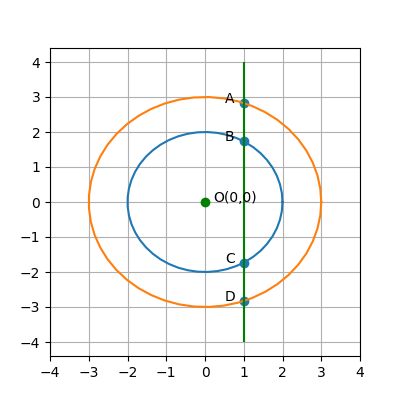
\includegraphics[width = \columnwidth]{chapters/9/10/4/4/figs/fig.png}
\caption{}
\label{fig:chapters/9/10/4/4/1}
\end{figure}

\item If two equal chords of a circle intersect within the circle, prove 
that the line joining the point of intersection to the centre makes equal 
angles with the chords.
%\label{chapters/9/10/4/6}
\\
\solution 
%\iffalse
\documentclass[journal,12pt,twocolumn]{IEEEtran}
\usepackage{setspace}
\usepackage{gensymb}
\singlespacing
\usepackage[cmex10]{amsmath}
\usepackage{amsthm}
\usepackage{mathrsfs}
\usepackage{txfonts}
\usepackage{stfloats}
\usepackage{bm}
\usepackage{cite}
\usepackage{cases}
\usepackage{subfig}
\usepackage{longtable}
\usepackage{multirow}
\usepackage{enumitem}
\usepackage{mathtools}
\usepackage{tikz}
\usepackage{circuitikz}
\usepackage{verbatim}
\usepackage[breaklinks=true]{hyperref}
\usepackage{tkz-euclide} % loads  TikZ and tkz-base
\usepackage{listings}
\usepackage{color}    
\usepackage{array}    
\usepackage{longtable}
\usepackage{calc}     
\usepackage{multirow} 
\usepackage{hhline}   
\usepackage{ifthen}   
\usepackage{lscape}     
\usepackage{chngcntr}
\DeclareMathOperator*{\Res}{Res}
\renewcommand\thesection{\arabic{section}}
\renewcommand\thesubsection{\thesection.\arabic{subsection}}
\renewcommand\thesubsubsection{\thesubsection.\arabic{subsubsection}}

\renewcommand\thesectiondis{\arabic{section}}
\renewcommand\thesubsectiondis{\thesectiondis.\arabic{subsection}}
\renewcommand\thesubsubsectiondis{\thesubsectiondis.\arabic{subsubsection}}
\renewcommand\thetable{\arabic{table}}
% correct bad hyphenation here
\hyphenation{op-tical net-works semi-conduc-tor}
\def\inputGnumericTable{}                                 %%

\lstset{
%language=C,
frame=single, 
breaklines=true,
columns=fullflexible
}
%\lstset{
%language=tex,
%frame=single, 
%breaklines=true
%}

\begin{document}
\newtheorem{theorem}{Theorem}[section]
\newtheorem{problem}{Problem}
\newtheorem{proposition}{Proposition}[section]
\newtheorem{lemma}{Lemma}[section]
\newtheorem{corollary}[theorem]{Corollary}
\newtheorem{example}{Example}[section]
\newtheorem{definition}[problem]{Definition}
\newcommand{\BEQA}{\begin{eqnarray}}
\newcommand{\EEQA}{\end{eqnarray}}
\newcommand{\define}{\stackrel{\triangle}{=}}
\bibliographystyle{IEEEtran}
\providecommand{\mbf}{\mathbf}
\providecommand{\pr}[1]{\ensuremath{\Pr\left(#1\right)}}
\providecommand{\qfunc}[1]{\ensuremath{Q\left(#1\right)}}
\providecommand{\sbrak}[1]{\ensuremath{{}\left[#1\right]}}
\providecommand{\lsbrak}[1]{\ensuremath{{}\left[#1\right.}}
\providecommand{\rsbrak}[1]{\ensuremath{{}\left.#1\right]}}
\providecommand{\brak}[1]{\ensuremath{\left(#1\right)}}
\providecommand{\lbrak}[1]{\ensuremath{\left(#1\right.}}
\providecommand{\rbrak}[1]{\ensuremath{\left.#1\right)}}
\providecommand{\cbrak}[1]{\ensuremath{\left\{#1\right\}}}
\providecommand{\lcbrak}[1]{\ensuremath{\left\{#1\right.}}
\providecommand{\rcbrak}[1]{\ensuremath{\left.#1\right\}}}
\theoremstyle{remark}
\newtheorem{rem}{Remark}
\newcommand{\sgn}{\mathop{\mathrm{sgn}}}
\providecommand{\abs}[1]{\left\vert#1\right\vert}
\providecommand{\res}[1]{\Res\displaylimits_{#1}} 
\providecommand{\norm}[1]{\left\lVert#1\right\rVert}
\providecommand{\mtx}[1]{\mathbf{#1}}
\providecommand{\mean}[1]{E\left[ #1 \right]}
\providecommand{\fourier}{\overset{\mathcal{F}}{ \rightleftharpoons}}
\providecommand{\system}[1]{\overset{\mathcal{#1}}{ \longleftrightarrow}}
\newcommand{\solution}{\noindent \textbf{Solution: }}
\newcommand{\cosec}{\,\text{cosec}\,}
\providecommand{\dec}[2]{\ensuremath{\overset{#1}{\underset{#2}{\gtrless}}}}
\newcommand{\myvec}[1]{\ensuremath{\begin{pmatrix}#1\end{pmatrix}}}
\newcommand{\mydet}[1]{\ensuremath{\begin{vmatrix}#1\end{vmatrix}}}
\let\vec\mathbf
\def\putbox#1#2#3{\makebox[0in][l]{\makebox[#1][l]{}\raisebox{\baselineskip}[0in][0in]{\raisebox{#2}[0in][0in]{#3}}}}
     \def\rightbox#1{\makebox[0in][r]{#1}}
     \def\centbox#1{\makebox[0in]{#1}}
     \def\topbox#1{\raisebox{-\baselineskip}[0in][0in]{#1}}
     \def\midbox#1{\raisebox{-0.5\baselineskip}[0in][0in]{#1}}

\vspace{3cm}
\title{Circle Assignment}
\author{Gautam Singh}
\maketitle
\bigskip

\begin{abstract}
    This document contains the solution to Question 6 of 
    Exercise 4 in Chapter 10 of the class 9 NCERT textbook.
\end{abstract}

\begin{enumerate}
    \item A circular park of radius 20 m is situated in a colony. Three boys 
    Ankur, Syed and David are sitting at equal distance on its boundary each 
    having a toy telephone in his hands to talk each other. Find the length of 
    the string of each phone.

    \solution 
    \fi
		Let the position vectors of the boys be
    \begin{align}
        \vec{A} = \myvec{r\\0},\ \vec{S} = \myvec{r\cos\beta\\r\sin\beta},\ \vec{D} = \myvec{r\cos\gamma\\r\sin\gamma}
        \label{eq:chapters/9/10/4/6/pos-vec-def}
    \end{align}
    where
    \begin{align}
        \beta, \gamma \in \brak{0,2\pi}
        \label{eq:chapters/9/10/4/6/int}
    \end{align}
    We have,
    \begin{align}
        \norm{\vec{A}-\vec{S}}^2 &= \norm{\vec{A}-\vec{D}}^2 \\
        \implies \vec{A}^\top\vec{S} &= \vec{A}^\top\vec{D} \\
        \implies \cos\beta &= \cos\gamma \\
        \implies \beta = 2n\pi \pm \gamma
        \label{eq:chapters/9/10/4/6/bg-gen}
    \end{align}
    where $n \in \mathbb{Z}$. From \eqref{eq:chapters/9/10/4/6/int}, we force $n = 1$
    and consider the negative sign to get
    \begin{align}
        \beta+\gamma = 2\pi
        \label{eq:chapters/9/10/4/6/bg-sum}
    \end{align}
    Therefore, using \eqref{eq:chapters/9/10/4/6/bg-sum}
    \begin{align}
        \norm{\vec{A}-\vec{S}}^2 &= \norm{\vec{S}-\vec{D}}^2 \\
        \implies \vec{A}^\top\vec{S} &= \vec{D}^\top\vec{S} \\
        \implies \cos\beta &= \cos\brak{\beta-\gamma} \\
        \implies 2\beta-2\pi &= 2m\pi\pm\beta \\
        \implies 2\beta\pm\beta &= 2k\pi
        \label{eq:chapters/9/10/4/6/beta-eqn}
    \end{align}
    where $k \in \mathbb{Z}$. From \eqref{eq:chapters/9/10/4/6/int}, we can only consider
    the plus sign and $k \in \cbrak{1,2}$ to get
    \begin{align}
        \beta,\gamma \in \cbrak{\frac{2\pi}{3},\frac{4\pi}{3}}
        \label{eq:chapters/9/10/4/6/bg-sol}
    \end{align}
    Therefore, the length of the thread from \eqref{eq:chapters/9/10/4/6/bg-sol} is
    \begin{align}
        \norm{\vec{S}-\vec{D}} &= \norm{r\myvec{\cos\beta-\cos\gamma\\\sin\beta-\sin\gamma}} \\
                               &= r\sqrt{3}
    \end{align}
    Here, $r = 20$ m. Thus, the length is $20\sqrt{3}$ m.

    The situation is demonstrated in Fig. \ref{fig:chapters/9/10/4/6/equilateral}, plotted by the 
    Python code \texttt{codes/equilateral.py}. The values used for 
    construction are shown in Table \ref{tab:chapters/9/10/4/6/param}.
    \begin{table}[!ht]
        \centering
        %%%%%%%%%%%%%%%%%%%%%%%%%%%%%%%%%%%%%%%%%%%%%%%%%%%%%%%%%%%%%%%%%%%%%%
%%                                                                  %%
%%  This is the header of a LaTeX2e file exported from Gnumeric.    %%
%%                                                                  %%
%%  This file can be compiled as it stands or included in another   %%
%%  LaTeX document. The table is based on the longtable package so  %%
%%  the longtable options (headers, footers...) can be set in the   %%
%%  preamble section below (see PRAMBLE).                           %%
%%                                                                  %%
%%  To include the file in another, the following two lines must be %%
%%  in the including file:                                          %%
%%        \def\inputGnumericTable{}                                 %%
%%  at the beginning of the file and:                               %%
%%        \input{name-of-this-file.tex}                             %%
%%  where the table is to be placed. Note also that the including   %%
%%  file must use the following packages for the table to be        %%
%%  rendered correctly:                                             %%
%%    \usepackage[latin1]{inputenc}                                 %%
%%    \usepackage{color}                                            %%
%%    \usepackage{array}                                            %%
%%    \usepackage{longtable}                                        %%
%%    \usepackage{calc}                                             %%
%%    \usepackage{multirow}                                         %%
%%    \usepackage{hhline}                                           %%
%%    \usepackage{ifthen}                                           %%
%%  optionally (for landscape tables embedded in another document): %%
%%    \usepackage{lscape}                                           %%
%%                                                                  %%
%%%%%%%%%%%%%%%%%%%%%%%%%%%%%%%%%%%%%%%%%%%%%%%%%%%%%%%%%%%%%%%%%%%%%%



%%  This section checks if we are begin input into another file or  %%
%%  the file will be compiled alone. First use a macro taken from   %%
%%  the TeXbook ex 7.7 (suggestion of Han-Wen Nienhuys).            %%
\def\ifundefined#1{\expandafter\ifx\csname#1\endcsname\relax}


%%  Check for the \def token for inputed files. If it is not        %%
%%  defined, the file will be processed as a standalone and the     %%
%%  preamble will be used.                                          %%
\ifundefined{inputGnumericTable}

%%  We must be able to close or not the document at the end.        %%
	\def\gnumericTableEnd{\end{document}}


%%%%%%%%%%%%%%%%%%%%%%%%%%%%%%%%%%%%%%%%%%%%%%%%%%%%%%%%%%%%%%%%%%%%%%
%%                                                                  %%
%%  This is the PREAMBLE. Change these values to get the right      %%
%%  paper size and other niceties.                                  %%
%%                                                                  %%
%%%%%%%%%%%%%%%%%%%%%%%%%%%%%%%%%%%%%%%%%%%%%%%%%%%%%%%%%%%%%%%%%%%%%%

	\documentclass[12pt%
			  %,landscape%
                    ]{report}
       \usepackage[latin1]{inputenc}
       \usepackage{fullpage}
       \usepackage{color}
       \usepackage{array}
       \usepackage{longtable}
       \usepackage{calc}
       \usepackage{multirow}
       \usepackage{hhline}
       \usepackage{ifthen}

	\begin{document}


%%  End of the preamble for the standalone. The next section is for %%
%%  documents which are included into other LaTeX2e files.          %%
\else

%%  We are not a stand alone document. For a regular table, we will %%
%%  have no preamble and only define the closing to mean nothing.   %%
    \def\gnumericTableEnd{}

%%  If we want landscape mode in an embedded document, comment out  %%
%%  the line above and uncomment the two below. The table will      %%
%%  begin on a new page and run in landscape mode.                  %%
%       \def\gnumericTableEnd{\end{landscape}}
%       \begin{landscape}


%%  End of the else clause for this file being \input.              %%
\fi

%%%%%%%%%%%%%%%%%%%%%%%%%%%%%%%%%%%%%%%%%%%%%%%%%%%%%%%%%%%%%%%%%%%%%%
%%                                                                  %%
%%  The rest is the gnumeric table, except for the closing          %%
%%  statement. Changes below will alter the table's appearance.     %%
%%                                                                  %%
%%%%%%%%%%%%%%%%%%%%%%%%%%%%%%%%%%%%%%%%%%%%%%%%%%%%%%%%%%%%%%%%%%%%%%

\providecommand{\gnumericmathit}[1]{#1} 
%%  Uncomment the next line if you would like your numbers to be in %%
%%  italics if they are italizised in the gnumeric table.           %%
%\renewcommand{\gnumericmathit}[1]{\mathit{#1}}
\providecommand{\gnumericPB}[1]%
{\let\gnumericTemp=\\#1\let\\=\gnumericTemp\hspace{0pt}}
 \ifundefined{gnumericTableWidthDefined}
        \newlength{\gnumericTableWidth}
        \newlength{\gnumericTableWidthComplete}
        \newlength{\gnumericMultiRowLength}
        \global\def\gnumericTableWidthDefined{}
 \fi
%% The following setting protects this code from babel shorthands.  %%
 \ifthenelse{\isundefined{\languageshorthands}}{}{\languageshorthands{english}}
%%  The default table format retains the relative column widths of  %%
%%  gnumeric. They can easily be changed to c, r or l. In that case %%
%%  you may want to comment out the next line and uncomment the one %%
%%  thereafter                                                      %%
\providecommand\gnumbox{\makebox[0pt]}
%%\providecommand\gnumbox[1][]{\makebox}

%% to adjust positions in multirow situations                       %%
\setlength{\bigstrutjot}{\jot}
\setlength{\extrarowheight}{\doublerulesep}

%%  The \setlongtables command keeps column widths the same across  %%
%%  pages. Simply comment out next line for varying column widths.  %%
\setlongtables

\setlength\gnumericTableWidth{%
	62pt+%
	67pt+%
0pt}
\def\gumericNumCols{2}
\setlength\gnumericTableWidthComplete{\gnumericTableWidth+%
         \tabcolsep*\gumericNumCols*2+\arrayrulewidth*\gumericNumCols}
\ifthenelse{\lengthtest{\gnumericTableWidthComplete > \linewidth}}%
         {\def\gnumericScale{1*\ratio{\linewidth-%
                        \tabcolsep*\gumericNumCols*2-%
                        \arrayrulewidth*\gumericNumCols}%
{\gnumericTableWidth}}}%
{\def\gnumericScale{1}}

%%%%%%%%%%%%%%%%%%%%%%%%%%%%%%%%%%%%%%%%%%%%%%%%%%%%%%%%%%%%%%%%%%%%%%
%%                                                                  %%
%% The following are the widths of the various columns. We are      %%
%% defining them here because then they are easier to change.       %%
%% Depending on the cell formats we may use them more than once.    %%
%%                                                                  %%
%%%%%%%%%%%%%%%%%%%%%%%%%%%%%%%%%%%%%%%%%%%%%%%%%%%%%%%%%%%%%%%%%%%%%%

\ifthenelse{\isundefined{\gnumericColA}}{\newlength{\gnumericColA}}{}\settowidth{\gnumericColA}{\begin{tabular}{@{}p{62pt*\gnumericScale}@{}}x\end{tabular}}
\ifthenelse{\isundefined{\gnumericColB}}{\newlength{\gnumericColB}}{}\settowidth{\gnumericColB}{\begin{tabular}{@{}p{67pt*\gnumericScale}@{}}x\end{tabular}}

\begin{tabular}[c]{%
	b{\gnumericColA}%
	b{\gnumericColB}%
	}

%%%%%%%%%%%%%%%%%%%%%%%%%%%%%%%%%%%%%%%%%%%%%%%%%%%%%%%%%%%%%%%%%%%%%%
%%  The longtable options. (Caption, headers... see Goosens, p.124) %%
%	\caption{The Table Caption.}             \\	%
% \hline	% Across the top of the table.
%%  The rest of these options are table rows which are placed on    %%
%%  the first, last or every page. Use \multicolumn if you want.    %%

%%  Header for the first page.                                      %%
%	\multicolumn{2}{c}{The First Header} \\ \hline 
%	\multicolumn{1}{c}{colTag}	%Column 1
%	&\multicolumn{1}{c}{colTag}	\\ \hline %Last column
%	\endfirsthead

%%  The running header definition.                                  %%
%	\hline
%	\multicolumn{2}{l}{\ldots\small\slshape continued} \\ \hline
%	\multicolumn{1}{c}{colTag}	%Column 1
%	&\multicolumn{1}{c}{colTag}	\\ \hline %Last column
%	\endhead

%%  The running footer definition.                                  %%
%	\hline
%	\multicolumn{2}{r}{\small\slshape continued\ldots} \\
%	\endfoot

%%  The ending footer definition.                                   %%
%	\multicolumn{2}{c}{That's all folks} \\ \hline 
%	\endlastfoot
%%%%%%%%%%%%%%%%%%%%%%%%%%%%%%%%%%%%%%%%%%%%%%%%%%%%%%%%%%%%%%%%%%%%%%

\hhline{|-|-}
	 \multicolumn{1}{|p{\gnumericColA}|}%
	{\gnumericPB{\centering}\gnumbox{\textbf{Parameter}}}
	&\multicolumn{1}{p{\gnumericColB}|}%
	{\gnumericPB{\centering}\gnumbox{\textbf{Value}}}
\\
\hhline{|--|}
	 \multicolumn{1}{|p{\gnumericColA}|}%
	{\gnumericPB{\centering}\gnumbox{$r$}}
	&\multicolumn{1}{p{\gnumericColB}|}%
	{\gnumericPB{\centering}\gnumbox{20}}
\\
\hhline{|--|}
	 \multicolumn{1}{|p{\gnumericColA}|}%
	{\gnumericPB{\centering}\gnumbox{$\beta$}}
	&\multicolumn{1}{p{\gnumericColB}|}%
    {\gnumericPB{\centering}\gnumbox{$\frac{2\pi}{3}$}}
\\
\hhline{|--|}
	 \multicolumn{1}{|p{\gnumericColA}|}%
	{\gnumericPB{\centering}\gnumbox{$\gamma$}}
	&\multicolumn{1}{p{\gnumericColB}|}%
    {\gnumericPB{\centering}\gnumbox{$\frac{4\pi}{3}$}}
\\
\hhline{|--|}
	 \multicolumn{1}{|p{\gnumericColA}|}%
     {\gnumericPB{\centering}\gnumbox{$\vec{O}$}}
	&\multicolumn{1}{p{\gnumericColB}|}%
    {\gnumericPB{\centering}\gnumbox{$\myvec{0\\0}$}}
\\
\hhline{|-|-|}
\end{tabular}

\ifthenelse{\isundefined{\languageshorthands}}{}{\languageshorthands{\languagename}}
\gnumericTableEnd

        \caption{Parameters used in the construction of Fig. \ref{fig:chapters/9/10/4/6/equilateral}.}
        \label{tab:chapters/9/10/4/6/param}
    \end{table}
    \begin{figure}[!ht]
        \centering
        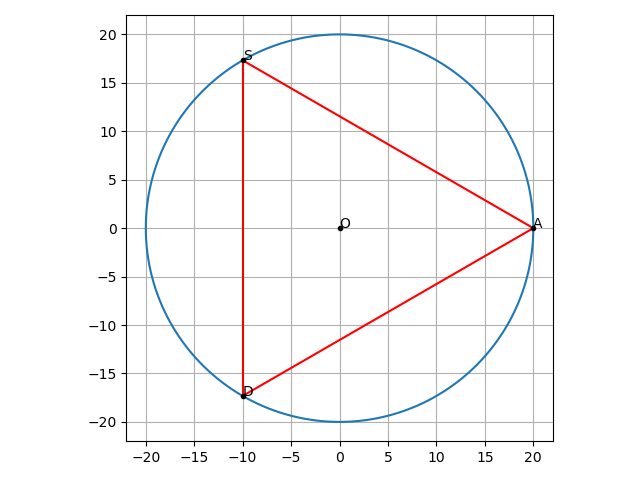
\includegraphics[width=\columnwidth]{chapters/9/10/4/6/figs/equilateral.png}
        \caption{$ASD$ is an equilateral triangle of side $20\sqrt{3}$ m.}
        \label{fig:chapters/9/10/4/6/equilateral}
    \end{figure}

\item If a line intersects two concentric circles (circles with the same 
centre) with centre $\vec{O}$ at $\vec{A}, \vec{B}, \vec{C}, \vec{D}$, prove 
that $AB = CD$ (see Fig. 
		\ref{fig:chapters/9/10/41} ).
\begin{figure}[!ht]
    \centering
    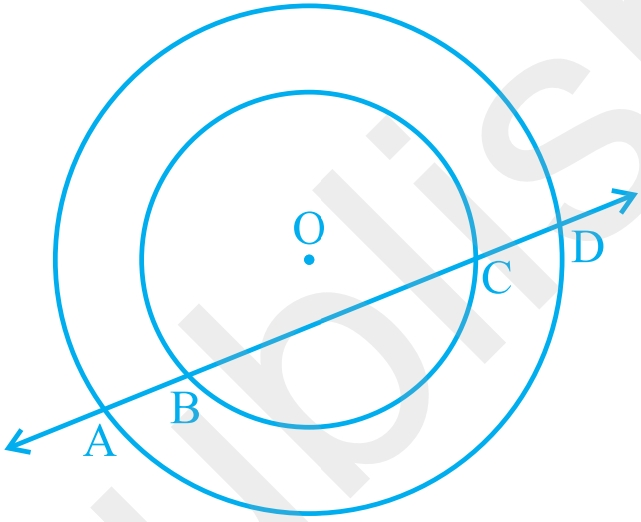
\includegraphics[width=\columnwidth]{chapters/9/10/4/figs/fig1.jpg}
    \caption{}
    \label{fig:chapters/9/10/41}
\end{figure}
\item Three girls Reshma, Salma and Mandip are playing a game by standing on 
a circle of radius 5m drawn in a park. Reshma throws a ball to Salma, Salma to 
Mandip, Mandip to Reshma. If the distance between Reshma and Salma and between 
Salma and Mandip is 6m each, what is the distance between Reshma and Mandip?
\\
\solution 
\iffalse
\documentclass[journal,12pt,twocolumn]{IEEEtran}
%
\usepackage{setspace}
\usepackage{gensymb}
%\doublespacing
\singlespacing

%\usepackage{graphicx}
%\usepackage{amssymb}
%\usepackage{relsize}
\usepackage[cmex10]{amsmath}
%\usepackage{amsthm}
%\interdisplaylinepenalty=2500
%\savesymbol{iint}
%\usepackage{txfonts}
%\restoresymbol{TXF}{iint}
%\usepackage{wasysym}
\usepackage{amsthm}
%\usepackage{iithtlc}
\usepackage{mathrsfs}
\usepackage{txfonts}
\usepackage{stfloats}
\usepackage{bm}
\usepackage{cite}
\usepackage{cases}
\usepackage{subfig}
%\usepackage{xtab}
\usepackage{longtable}
\usepackage{multirow}
%\usepackage{algorithm}
%\usepackage{algpseudocode}
\usepackage{enumitem}
\usepackage{mathtools}
\usepackage{steinmetz}
\usepackage{tikz}
\usepackage{circuitikz}
\usepackage{verbatim}
\usepackage{tfrupee}
\usepackage[breaklinks=true]{hyperref}
%\usepackage{stmaryrd}
\usepackage{tkz-euclide} % loads  TikZ and tkz-base
%\usetkzobj{all}
\usetikzlibrary{calc,math}
\usepackage{listings}
    \usepackage{color}                                            %%
    \usepackage{array}                                            %%
    \usepackage{longtable}                                        %%
    \usepackage{calc}                                             %%
    \usepackage{multirow}                                         %%
    \usepackage{hhline}                                           %%
    \usepackage{ifthen}                                           %%
  %optionally (for landscape tables embedded in another document): %%
    \usepackage{lscape}     
\usepackage{multicol}
\usepackage{chngcntr}
%\usepackage{enumerate}

%\usepackage{wasysym}
%\newcounter{MYtempeqncnt}
\DeclareMathOperator*{\Res}{Res}
%\renewcommand{\baselinestretch}{2}
\renewcommand\thesection{\arabic{section}}
\renewcommand\thesubsection{\thesection.\arabic{subsection}}
\renewcommand\thesubsubsection{\thesubsection.\arabic{subsubsection}}

\renewcommand\thesectiondis{\arabic{section}}
\renewcommand\thesubsectiondis{\thesectiondis.\arabic{subsection}}
\renewcommand\thesubsubsectiondis{\thesubsectiondis.\arabic{subsubsection}}

% correct bad hyphenation here
\hyphenation{op-tical net-works semi-conduc-tor}
\def\inputGnumericTable{}                                 %%

\lstset{
%language=C,
frame=single, 
breaklines=true,
columns=fullflexible
}
%\lstset{
%language=tex,
%frame=single, 
%breaklines=true
%}

\begin{document}
%


\newtheorem{theorem}{Theorem}[section]
\newtheorem{problem}{Problem}
\newtheorem{proposition}{Proposition}[section]
\newtheorem{lemma}{Lemma}[section]
\newtheorem{corollary}[theorem]{Corollary}
\newtheorem{example}{Example}[section]
\newtheorem{definition}[problem]{Definition}
%\newtheorem{thm}{Theorem}[section] 
%\newtheorem{defn}[thm]{Definition}
%\newtheorem{algorithm}{Algorithm}[section]
%\newtheorem{cor}{Corollary}
\newcommand{\BEQA}{\begin{eqnarray}}
\newcommand{\EEQA}{\end{eqnarray}}
\newcommand{\define}{\stackrel{\triangle}{=}}

\bibliographystyle{IEEEtran}
%\bibliographystyle{ieeetr}


\providecommand{\mbf}{\mathbf}
\providecommand{\pr}[1]{\ensuremath{\Pr\left(#1\right)}}
\providecommand{\qfunc}[1]{\ensuremath{Q\left(#1\right)}}
\providecommand{\sbrak}[1]{\ensuremath{{}\left[#1\right]}}
\providecommand{\lsbrak}[1]{\ensuremath{{}\left[#1\right.}}
\providecommand{\rsbrak}[1]{\ensuremath{{}\left.#1\right]}}
\providecommand{\brak}[1]{\ensuremath{\left(#1\right)}}
\providecommand{\lbrak}[1]{\ensuremath{\left(#1\right.}}
\providecommand{\rbrak}[1]{\ensuremath{\left.#1\right)}}
\providecommand{\cbrak}[1]{\ensuremath{\left\{#1\right\}}}
\providecommand{\lcbrak}[1]{\ensuremath{\left\{#1\right.}}
\providecommand{\rcbrak}[1]{\ensuremath{\left.#1\right\}}}
\theoremstyle{remark}
\newtheorem{rem}{Remark}
\newcommand{\sgn}{\mathop{\mathrm{sgn}}}
\providecommand{\abs}[1]{\left\vert#1\right\vert}
\providecommand{\res}[1]{\Res\displaylimits_{#1}} 
\providecommand{\norm}[1]{\left\lVert#1\right\rVert}
%\providecommand{\norm}[1]{\lVert#1\rVert}
\providecommand{\mtx}[1]{\mathbf{#1}}
\providecommand{\mean}[1]{E\left[ #1 \right]}
\providecommand{\fourier}{\overset{\mathcal{F}}{ \rightleftharpoons}}
%\providecommand{\hilbert}{\overset{\mathcal{H}}{ \rightleftharpoons}}
\providecommand{\system}{\overset{\mathcal{H}}{ \longleftrightarrow}}
	%\newcommand{\solution}[2]{\textbf{Solution:}{#1}}
\newcommand{\solution}{\noindent \textbf{Solution: }}
\newcommand{\cosec}{\,\text{cosec}\,}
\providecommand{\dec}[2]{\ensuremath{\overset{#1}{\underset{#2}{\gtrless}}}}
\newcommand{\myvec}[1]{\ensuremath{\begin{pmatrix}#1\end{pmatrix}}}
\newcommand{\mydet}[1]{\ensuremath{\begin{vmatrix}#1\end{vmatrix}}}
%\numberwithin{equation}{section}
\numberwithin{equation}{subsection}
%\numberwithin{problem}{section}
%\numberwithin{definition}{section}
\makeatletter
\@addtoreset{figure}{problem}
\makeatother

\let\StandardTheFigure\thefigure
\let\vec\mathbf
%\renewcommand{\thefigure}{\theproblem.\arabic{figure}}
\renewcommand{\thefigure}{\theproblem}
%\setlist[enumerate,1]{before=\renewcommand\theequation{\theenumi.\arabic{equation}}
%\counterwithin{equation}{enumi}


%\renewcommand{\theequation}{\arabic{subsection}.\arabic{equation}}

\def\putbox#1#2#3{\makebox[0in][l]{\makebox[#1][l]{}\raisebox{\baselineskip}[0in][0in]{\raisebox{#2}[0in][0in]{#3}}}}
     \def\rightbox#1{\makebox[0in][r]{#1}}
     \def\centbox#1{\makebox[0in]{#1}}
     \def\topbox#1{\raisebox{-\baselineskip}[0in][0in]{#1}}
     \def\midbox#1{\raisebox{-0.5\baselineskip}[0in][0in]{#1}}

\vspace{3cm}


\title{Question: 9.10.4.5}
\author{Nikam Pratik Balasaheb (EE21BTECH11037)}





% make the title area
\maketitle

\newpage

%\tableofcontents

\bigskip

\renewcommand{\thefigure}{\theenumi}
\renewcommand{\thetable}{\theenumi}
%\renewcommand{\theequation}{\theenumi}

\section{Problem}
Three girls Reshma, Salma and Mandip are playing a game by standing on a circle of radius 5m drawn in a park. Reshma throws a ball to Salma, Salma to Mandip, Mandip to Reshma. If the distance between Reshma and Salma and
between Salma and Mandip is 6m each, what is the distance between Reshma and Mandip?

\section{Solution}
\fi
Consider Reshma, Salma and Mandip be standing at $\vec{A}$, $\vec{B}$ and $\vec{C}$ respectively, and the center the of the circle $\vec{O}$.
The input parameters are listed in Table 
\ref{tab:chapters/9/10/4/5/}.
Let 
\begin{align}
	\vec{B} = \myvec{0\\0},\,
	\vec{O} = \myvec{5\\0}
\end{align}
Therefore, the equation of the cicle is given by 
\begin{align}
	\norm{\vec{x}-\vec{O}}^2 &= 25\\
\implies 	\norm{\vec{x}}^2 - 2 \vec{O}^{\top}\vec{x} + \norm{\vec{O}}^2 - 25 &= 0\\
\implies	\norm{\vec{x}}^2 - 2 \myvec{5 & 0}\vec{x} &= 0
	\label{eq:chapters/9/10/4/5/1}
\end{align}
Also, $\vec{A}$ and $\vec{C}$ are equidistant (6m) from $\vec{B}$, we can say that they lie on the circle having $\vec{B}$ as center and radius 6m. Equation of this circle is given by
\begin{align}
	\norm{\vec{x}}^2 - 2\vec{B}^{\top} \vec{x} + \norm{\vec{B}}^2 - 36 &= 0\\
	\norm{\vec{x}}^2 &= 36\\
	i.e., \vec{u} = \myvec{0\\0}\;, \; f = -36
	\label{eq:chapters/9/10/4/5/2}
\end{align}
From \eqref{eq:chapters/9/10/4/5/1} and \eqref{eq:chapters/9/10/4/5/2}, the line passing through $\vec{A}$ and $\vec{C}$  is
\begin{align}
	\myvec{5&0} \vec{x} &= 18\\
\implies 	\vec{x} &= \myvec{\frac{18}{5}\\[1pt] 0} + \mu \myvec{0\\1}\\
	i.e., \; \vec{h} = \myvec{\frac{18}{5}\\[1pt] 0} \; , \; \vec{m} = \myvec{0\\1}
\end{align}
For the circle,$\vec{V} = \vec{I}$
\begin{multline}
	\mu_i = \frac{1}{\vec{m}^{\top}\vec{V}\vec{m}} \brak{-m^{\top}\brak{\vec{V}\vec{h}+\vec{u}} \pm \sqrt{\brak{\vec{m}^{\top}\brak{\vec{V}\vec{h}+\vec{u}}}^2 - \text{g}\brak{\vec{h}}\brak{\vec{m}^{\top}\vec{V}\vec{m}}}}
\end{multline}
where,
\begin{align}
	\text{g}\brak{\vec{h}} = \vec{h}^{\top}\vec{V}\vec{h} + 2\vec{u}^{\top}\vec{h} +f
\end{align}
yielding
\begin{align}
	\mu_i = \pm \frac{24}{5}
\end{align}
Therefore,
\begin{align}
	\vec{A} = \myvec{\frac{18}{5}\\[1pt] \frac{24}{5}},\,
	\vec{C} = \myvec{\frac{18}{5}\\[1pt] -\frac{24}{5}}
\end{align}
and the 
distance between Reshma and Mandip is
\begin{align}
	\norm{\vec{A} - \vec{C}} = \norm{\myvec{0\\[1pt] \frac{48}{5}}}
	= \frac{48}{5}
\end{align}
\begin{table}[h!]
\begin{center}
	%%%%%%%%%%%%%%%%%%%%%%%%%%%%%%%%%%%%%%%%%%%%%%%%%%%%%%%%%%%%%%%%%%%%%%
%%                                                                  %%
%%  This is a LaTeX2e table fragment exported from Gnumeric.        %%
%%                                                                  %%
%%%%%%%%%%%%%%%%%%%%%%%%%%%%%%%%%%%%%%%%%%%%%%%%%%%%%%%%%%%%%%%%%%%%%%

\begin{tabular}[]{|c|c|c|}
\hline
$\vec{O}$	& $\myvec{5\\0}$ &Center of the given circle \\ \hline
$\vec{B}$	& $\myvec{0\\0}$ &Point where Salma is standing\\ \hline
$r$		& 5 & radius of given circle \\ \hline
$d$ 		& 6 & distance AB and BC\\ \hline
\end{tabular}

\end{center}
\caption{}
\label{tab:chapters/9/10/4/5/}
\end{table}
See Fig. 
    \ref{fig:chapters/9/10/4/5/}.
\begin{figure}[h!]
  \centering
    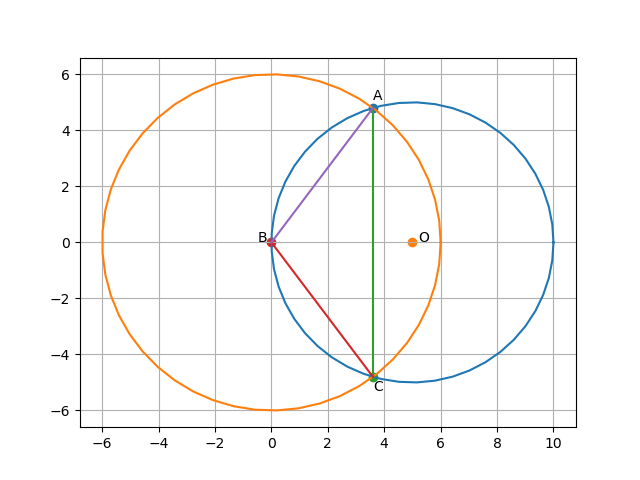
\includegraphics[width=\columnwidth]{chapters/9/10/4/5/figs/Figure_1.png}
    \caption{}
    \label{fig:chapters/9/10/4/5/}
\end{figure}





\item A circular park of radius 20m is situated in a colony. Three boys Ankur,
Syed and David are sitting at equal distance on its boundary each having a toy 
telephone in his hands to talk each other. Find the length of the string of each 
phone.
\item 
\label{chapters/9/10/4/6}
\iffalse
\documentclass[journal,12pt,twocolumn]{IEEEtran}
\usepackage{setspace}
\usepackage{gensymb}
\singlespacing
\usepackage[cmex10]{amsmath}
\usepackage{amsthm}
\usepackage{mathrsfs}
\usepackage{txfonts}
\usepackage{stfloats}
\usepackage{bm}
\usepackage{cite}
\usepackage{cases}
\usepackage{subfig}
\usepackage{longtable}
\usepackage{multirow}
\usepackage{enumitem}
\usepackage{mathtools}
\usepackage{tikz}
\usepackage{circuitikz}
\usepackage{verbatim}
\usepackage[breaklinks=true]{hyperref}
\usepackage{tkz-euclide} % loads  TikZ and tkz-base
\usepackage{listings}
\usepackage{color}    
\usepackage{array}    
\usepackage{longtable}
\usepackage{calc}     
\usepackage{multirow} 
\usepackage{hhline}   
\usepackage{ifthen}   
\usepackage{lscape}     
\usepackage{chngcntr}
\DeclareMathOperator*{\Res}{Res}
\renewcommand\thesection{\arabic{section}}
\renewcommand\thesubsection{\thesection.\arabic{subsection}}
\renewcommand\thesubsubsection{\thesubsection.\arabic{subsubsection}}

\renewcommand\thesectiondis{\arabic{section}}
\renewcommand\thesubsectiondis{\thesectiondis.\arabic{subsection}}
\renewcommand\thesubsubsectiondis{\thesubsectiondis.\arabic{subsubsection}}
\renewcommand\thetable{\arabic{table}}
% correct bad hyphenation here
\hyphenation{op-tical net-works semi-conduc-tor}
\def\inputGnumericTable{}                                 %%

\lstset{
%language=C,
frame=single, 
breaklines=true,
columns=fullflexible
}
%\lstset{
%language=tex,
%frame=single, 
%breaklines=true
%}

\begin{document}
\newtheorem{theorem}{Theorem}[section]
\newtheorem{problem}{Problem}
\newtheorem{proposition}{Proposition}[section]
\newtheorem{lemma}{Lemma}[section]
\newtheorem{corollary}[theorem]{Corollary}
\newtheorem{example}{Example}[section]
\newtheorem{definition}[problem]{Definition}
\newcommand{\BEQA}{\begin{eqnarray}}
\newcommand{\EEQA}{\end{eqnarray}}
\newcommand{\define}{\stackrel{\triangle}{=}}
\bibliographystyle{IEEEtran}
\providecommand{\mbf}{\mathbf}
\providecommand{\pr}[1]{\ensuremath{\Pr\left(#1\right)}}
\providecommand{\qfunc}[1]{\ensuremath{Q\left(#1\right)}}
\providecommand{\sbrak}[1]{\ensuremath{{}\left[#1\right]}}
\providecommand{\lsbrak}[1]{\ensuremath{{}\left[#1\right.}}
\providecommand{\rsbrak}[1]{\ensuremath{{}\left.#1\right]}}
\providecommand{\brak}[1]{\ensuremath{\left(#1\right)}}
\providecommand{\lbrak}[1]{\ensuremath{\left(#1\right.}}
\providecommand{\rbrak}[1]{\ensuremath{\left.#1\right)}}
\providecommand{\cbrak}[1]{\ensuremath{\left\{#1\right\}}}
\providecommand{\lcbrak}[1]{\ensuremath{\left\{#1\right.}}
\providecommand{\rcbrak}[1]{\ensuremath{\left.#1\right\}}}
\theoremstyle{remark}
\newtheorem{rem}{Remark}
\newcommand{\sgn}{\mathop{\mathrm{sgn}}}
\providecommand{\abs}[1]{\left\vert#1\right\vert}
\providecommand{\res}[1]{\Res\displaylimits_{#1}} 
\providecommand{\norm}[1]{\left\lVert#1\right\rVert}
\providecommand{\mtx}[1]{\mathbf{#1}}
\providecommand{\mean}[1]{E\left[ #1 \right]}
\providecommand{\fourier}{\overset{\mathcal{F}}{ \rightleftharpoons}}
\providecommand{\system}[1]{\overset{\mathcal{#1}}{ \longleftrightarrow}}
\newcommand{\solution}{\noindent \textbf{Solution: }}
\newcommand{\cosec}{\,\text{cosec}\,}
\providecommand{\dec}[2]{\ensuremath{\overset{#1}{\underset{#2}{\gtrless}}}}
\newcommand{\myvec}[1]{\ensuremath{\begin{pmatrix}#1\end{pmatrix}}}
\newcommand{\mydet}[1]{\ensuremath{\begin{vmatrix}#1\end{vmatrix}}}
\let\vec\mathbf
\def\putbox#1#2#3{\makebox[0in][l]{\makebox[#1][l]{}\raisebox{\baselineskip}[0in][0in]{\raisebox{#2}[0in][0in]{#3}}}}
     \def\rightbox#1{\makebox[0in][r]{#1}}
     \def\centbox#1{\makebox[0in]{#1}}
     \def\topbox#1{\raisebox{-\baselineskip}[0in][0in]{#1}}
     \def\midbox#1{\raisebox{-0.5\baselineskip}[0in][0in]{#1}}

\vspace{3cm}
\title{Circle Assignment}
\author{Gautam Singh}
\maketitle
\bigskip

\begin{abstract}
    This document contains the solution to Question 6 of 
    Exercise 4 in Chapter 10 of the class 9 NCERT textbook.
\end{abstract}

\begin{enumerate}
    \item A circular park of radius 20 m is situated in a colony. Three boys 
    Ankur, Syed and David are sitting at equal distance on its boundary each 
    having a toy telephone in his hands to talk each other. Find the length of 
    the string of each phone.

    \solution 
    \fi
		Let the position vectors of the boys be
    \begin{align}
        \vec{A} = \myvec{r\\0},\ \vec{S} = \myvec{r\cos\beta\\r\sin\beta},\ \vec{D} = \myvec{r\cos\gamma\\r\sin\gamma}
        \label{eq:chapters/9/10/4/6/pos-vec-def}
    \end{align}
    where
    \begin{align}
        \beta, \gamma \in \brak{0,2\pi}
        \label{eq:chapters/9/10/4/6/int}
    \end{align}
    We have,
    \begin{align}
        \norm{\vec{A}-\vec{S}}^2 &= \norm{\vec{A}-\vec{D}}^2 \\
        \implies \vec{A}^\top\vec{S} &= \vec{A}^\top\vec{D} \\
        \implies \cos\beta &= \cos\gamma \\
        \implies \beta = 2n\pi \pm \gamma
        \label{eq:chapters/9/10/4/6/bg-gen}
    \end{align}
    where $n \in \mathbb{Z}$. From \eqref{eq:chapters/9/10/4/6/int}, we force $n = 1$
    and consider the negative sign to get
    \begin{align}
        \beta+\gamma = 2\pi
        \label{eq:chapters/9/10/4/6/bg-sum}
    \end{align}
    Therefore, using \eqref{eq:chapters/9/10/4/6/bg-sum}
    \begin{align}
        \norm{\vec{A}-\vec{S}}^2 &= \norm{\vec{S}-\vec{D}}^2 \\
        \implies \vec{A}^\top\vec{S} &= \vec{D}^\top\vec{S} \\
        \implies \cos\beta &= \cos\brak{\beta-\gamma} \\
        \implies 2\beta-2\pi &= 2m\pi\pm\beta \\
        \implies 2\beta\pm\beta &= 2k\pi
        \label{eq:chapters/9/10/4/6/beta-eqn}
    \end{align}
    where $k \in \mathbb{Z}$. From \eqref{eq:chapters/9/10/4/6/int}, we can only consider
    the plus sign and $k \in \cbrak{1,2}$ to get
    \begin{align}
        \beta,\gamma \in \cbrak{\frac{2\pi}{3},\frac{4\pi}{3}}
        \label{eq:chapters/9/10/4/6/bg-sol}
    \end{align}
    Therefore, the length of the thread from \eqref{eq:chapters/9/10/4/6/bg-sol} is
    \begin{align}
        \norm{\vec{S}-\vec{D}} &= \norm{r\myvec{\cos\beta-\cos\gamma\\\sin\beta-\sin\gamma}} \\
                               &= r\sqrt{3}
    \end{align}
    Here, $r = 20$ m. Thus, the length is $20\sqrt{3}$ m.

    The situation is demonstrated in Fig. \ref{fig:chapters/9/10/4/6/equilateral}, plotted by the 
    Python code \texttt{codes/equilateral.py}. The values used for 
    construction are shown in Table \ref{tab:chapters/9/10/4/6/param}.
    \begin{table}[!ht]
        \centering
        %%%%%%%%%%%%%%%%%%%%%%%%%%%%%%%%%%%%%%%%%%%%%%%%%%%%%%%%%%%%%%%%%%%%%%
%%                                                                  %%
%%  This is the header of a LaTeX2e file exported from Gnumeric.    %%
%%                                                                  %%
%%  This file can be compiled as it stands or included in another   %%
%%  LaTeX document. The table is based on the longtable package so  %%
%%  the longtable options (headers, footers...) can be set in the   %%
%%  preamble section below (see PRAMBLE).                           %%
%%                                                                  %%
%%  To include the file in another, the following two lines must be %%
%%  in the including file:                                          %%
%%        \def\inputGnumericTable{}                                 %%
%%  at the beginning of the file and:                               %%
%%        \input{name-of-this-file.tex}                             %%
%%  where the table is to be placed. Note also that the including   %%
%%  file must use the following packages for the table to be        %%
%%  rendered correctly:                                             %%
%%    \usepackage[latin1]{inputenc}                                 %%
%%    \usepackage{color}                                            %%
%%    \usepackage{array}                                            %%
%%    \usepackage{longtable}                                        %%
%%    \usepackage{calc}                                             %%
%%    \usepackage{multirow}                                         %%
%%    \usepackage{hhline}                                           %%
%%    \usepackage{ifthen}                                           %%
%%  optionally (for landscape tables embedded in another document): %%
%%    \usepackage{lscape}                                           %%
%%                                                                  %%
%%%%%%%%%%%%%%%%%%%%%%%%%%%%%%%%%%%%%%%%%%%%%%%%%%%%%%%%%%%%%%%%%%%%%%



%%  This section checks if we are begin input into another file or  %%
%%  the file will be compiled alone. First use a macro taken from   %%
%%  the TeXbook ex 7.7 (suggestion of Han-Wen Nienhuys).            %%
\def\ifundefined#1{\expandafter\ifx\csname#1\endcsname\relax}


%%  Check for the \def token for inputed files. If it is not        %%
%%  defined, the file will be processed as a standalone and the     %%
%%  preamble will be used.                                          %%
\ifundefined{inputGnumericTable}

%%  We must be able to close or not the document at the end.        %%
	\def\gnumericTableEnd{\end{document}}


%%%%%%%%%%%%%%%%%%%%%%%%%%%%%%%%%%%%%%%%%%%%%%%%%%%%%%%%%%%%%%%%%%%%%%
%%                                                                  %%
%%  This is the PREAMBLE. Change these values to get the right      %%
%%  paper size and other niceties.                                  %%
%%                                                                  %%
%%%%%%%%%%%%%%%%%%%%%%%%%%%%%%%%%%%%%%%%%%%%%%%%%%%%%%%%%%%%%%%%%%%%%%

	\documentclass[12pt%
			  %,landscape%
                    ]{report}
       \usepackage[latin1]{inputenc}
       \usepackage{fullpage}
       \usepackage{color}
       \usepackage{array}
       \usepackage{longtable}
       \usepackage{calc}
       \usepackage{multirow}
       \usepackage{hhline}
       \usepackage{ifthen}

	\begin{document}


%%  End of the preamble for the standalone. The next section is for %%
%%  documents which are included into other LaTeX2e files.          %%
\else

%%  We are not a stand alone document. For a regular table, we will %%
%%  have no preamble and only define the closing to mean nothing.   %%
    \def\gnumericTableEnd{}

%%  If we want landscape mode in an embedded document, comment out  %%
%%  the line above and uncomment the two below. The table will      %%
%%  begin on a new page and run in landscape mode.                  %%
%       \def\gnumericTableEnd{\end{landscape}}
%       \begin{landscape}


%%  End of the else clause for this file being \input.              %%
\fi

%%%%%%%%%%%%%%%%%%%%%%%%%%%%%%%%%%%%%%%%%%%%%%%%%%%%%%%%%%%%%%%%%%%%%%
%%                                                                  %%
%%  The rest is the gnumeric table, except for the closing          %%
%%  statement. Changes below will alter the table's appearance.     %%
%%                                                                  %%
%%%%%%%%%%%%%%%%%%%%%%%%%%%%%%%%%%%%%%%%%%%%%%%%%%%%%%%%%%%%%%%%%%%%%%

\providecommand{\gnumericmathit}[1]{#1} 
%%  Uncomment the next line if you would like your numbers to be in %%
%%  italics if they are italizised in the gnumeric table.           %%
%\renewcommand{\gnumericmathit}[1]{\mathit{#1}}
\providecommand{\gnumericPB}[1]%
{\let\gnumericTemp=\\#1\let\\=\gnumericTemp\hspace{0pt}}
 \ifundefined{gnumericTableWidthDefined}
        \newlength{\gnumericTableWidth}
        \newlength{\gnumericTableWidthComplete}
        \newlength{\gnumericMultiRowLength}
        \global\def\gnumericTableWidthDefined{}
 \fi
%% The following setting protects this code from babel shorthands.  %%
 \ifthenelse{\isundefined{\languageshorthands}}{}{\languageshorthands{english}}
%%  The default table format retains the relative column widths of  %%
%%  gnumeric. They can easily be changed to c, r or l. In that case %%
%%  you may want to comment out the next line and uncomment the one %%
%%  thereafter                                                      %%
\providecommand\gnumbox{\makebox[0pt]}
%%\providecommand\gnumbox[1][]{\makebox}

%% to adjust positions in multirow situations                       %%
\setlength{\bigstrutjot}{\jot}
\setlength{\extrarowheight}{\doublerulesep}

%%  The \setlongtables command keeps column widths the same across  %%
%%  pages. Simply comment out next line for varying column widths.  %%
\setlongtables

\setlength\gnumericTableWidth{%
	62pt+%
	67pt+%
0pt}
\def\gumericNumCols{2}
\setlength\gnumericTableWidthComplete{\gnumericTableWidth+%
         \tabcolsep*\gumericNumCols*2+\arrayrulewidth*\gumericNumCols}
\ifthenelse{\lengthtest{\gnumericTableWidthComplete > \linewidth}}%
         {\def\gnumericScale{1*\ratio{\linewidth-%
                        \tabcolsep*\gumericNumCols*2-%
                        \arrayrulewidth*\gumericNumCols}%
{\gnumericTableWidth}}}%
{\def\gnumericScale{1}}

%%%%%%%%%%%%%%%%%%%%%%%%%%%%%%%%%%%%%%%%%%%%%%%%%%%%%%%%%%%%%%%%%%%%%%
%%                                                                  %%
%% The following are the widths of the various columns. We are      %%
%% defining them here because then they are easier to change.       %%
%% Depending on the cell formats we may use them more than once.    %%
%%                                                                  %%
%%%%%%%%%%%%%%%%%%%%%%%%%%%%%%%%%%%%%%%%%%%%%%%%%%%%%%%%%%%%%%%%%%%%%%

\ifthenelse{\isundefined{\gnumericColA}}{\newlength{\gnumericColA}}{}\settowidth{\gnumericColA}{\begin{tabular}{@{}p{62pt*\gnumericScale}@{}}x\end{tabular}}
\ifthenelse{\isundefined{\gnumericColB}}{\newlength{\gnumericColB}}{}\settowidth{\gnumericColB}{\begin{tabular}{@{}p{67pt*\gnumericScale}@{}}x\end{tabular}}

\begin{tabular}[c]{%
	b{\gnumericColA}%
	b{\gnumericColB}%
	}

%%%%%%%%%%%%%%%%%%%%%%%%%%%%%%%%%%%%%%%%%%%%%%%%%%%%%%%%%%%%%%%%%%%%%%
%%  The longtable options. (Caption, headers... see Goosens, p.124) %%
%	\caption{The Table Caption.}             \\	%
% \hline	% Across the top of the table.
%%  The rest of these options are table rows which are placed on    %%
%%  the first, last or every page. Use \multicolumn if you want.    %%

%%  Header for the first page.                                      %%
%	\multicolumn{2}{c}{The First Header} \\ \hline 
%	\multicolumn{1}{c}{colTag}	%Column 1
%	&\multicolumn{1}{c}{colTag}	\\ \hline %Last column
%	\endfirsthead

%%  The running header definition.                                  %%
%	\hline
%	\multicolumn{2}{l}{\ldots\small\slshape continued} \\ \hline
%	\multicolumn{1}{c}{colTag}	%Column 1
%	&\multicolumn{1}{c}{colTag}	\\ \hline %Last column
%	\endhead

%%  The running footer definition.                                  %%
%	\hline
%	\multicolumn{2}{r}{\small\slshape continued\ldots} \\
%	\endfoot

%%  The ending footer definition.                                   %%
%	\multicolumn{2}{c}{That's all folks} \\ \hline 
%	\endlastfoot
%%%%%%%%%%%%%%%%%%%%%%%%%%%%%%%%%%%%%%%%%%%%%%%%%%%%%%%%%%%%%%%%%%%%%%

\hhline{|-|-}
	 \multicolumn{1}{|p{\gnumericColA}|}%
	{\gnumericPB{\centering}\gnumbox{\textbf{Parameter}}}
	&\multicolumn{1}{p{\gnumericColB}|}%
	{\gnumericPB{\centering}\gnumbox{\textbf{Value}}}
\\
\hhline{|--|}
	 \multicolumn{1}{|p{\gnumericColA}|}%
	{\gnumericPB{\centering}\gnumbox{$r$}}
	&\multicolumn{1}{p{\gnumericColB}|}%
	{\gnumericPB{\centering}\gnumbox{20}}
\\
\hhline{|--|}
	 \multicolumn{1}{|p{\gnumericColA}|}%
	{\gnumericPB{\centering}\gnumbox{$\beta$}}
	&\multicolumn{1}{p{\gnumericColB}|}%
    {\gnumericPB{\centering}\gnumbox{$\frac{2\pi}{3}$}}
\\
\hhline{|--|}
	 \multicolumn{1}{|p{\gnumericColA}|}%
	{\gnumericPB{\centering}\gnumbox{$\gamma$}}
	&\multicolumn{1}{p{\gnumericColB}|}%
    {\gnumericPB{\centering}\gnumbox{$\frac{4\pi}{3}$}}
\\
\hhline{|--|}
	 \multicolumn{1}{|p{\gnumericColA}|}%
     {\gnumericPB{\centering}\gnumbox{$\vec{O}$}}
	&\multicolumn{1}{p{\gnumericColB}|}%
    {\gnumericPB{\centering}\gnumbox{$\myvec{0\\0}$}}
\\
\hhline{|-|-|}
\end{tabular}

\ifthenelse{\isundefined{\languageshorthands}}{}{\languageshorthands{\languagename}}
\gnumericTableEnd

        \caption{Parameters used in the construction of Fig. \ref{fig:chapters/9/10/4/6/equilateral}.}
        \label{tab:chapters/9/10/4/6/param}
    \end{table}
    \begin{figure}[!ht]
        \centering
        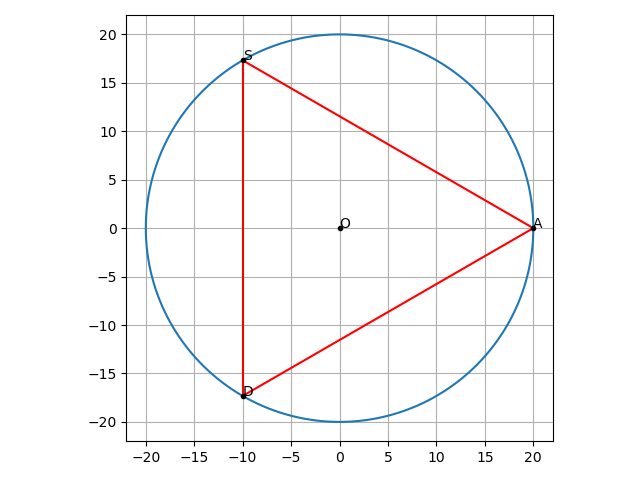
\includegraphics[width=\columnwidth]{chapters/9/10/4/6/figs/equilateral.png}
        \caption{$ASD$ is an equilateral triangle of side $20\sqrt{3}$ m.}
        \label{fig:chapters/9/10/4/6/equilateral}
    \end{figure}

\item  $\vec{A},\vec{B},\vec{C}$ are the three points on a circle with centre $\vec{O}$ such that $\angle$BOC=30\degree and $\angle$AOB=60\degree. If $\vec{D}$ is a point on the circle other than the arc ABC, find $\angle$ADC.
\label{chapters/9/10/5/1}
\\
\solution
\iffalse
\documentclass[12pt]{article}
\usepackage{graphicx}
\usepackage{amsmath}
\usepackage{mathtools}
\usepackage{gensymb}

\newcommand{\mydet}[1]{\ensuremath{\begin{vmatrix}#1\end{vmatrix}}}
\providecommand{\brak}[1]{\ensuremath{\left(#1\right)}}
\providecommand{\norm}[1]{\left\lVert#1\right\rVert}
\newcommand{\solution}{\noindent \textbf{Solution: }}
\newcommand{\myvec}[1]{\ensuremath{\begin{pmatrix}#1\end{pmatrix}}}
\let\vec\mathbf
\def\inputGnumericTable{}
\usepackage{color}                                            %%
    \usepackage{array}                                            %%
    \usepackage{longtable}                                        %%
    \usepackage{calc}                                             %%
    \usepackage{multirow}                                         %%
    \usepackage{hhline}                                           %%
    \usepackage{ifthen}
\usepackage{array}
\usepackage{amsmath}   % for having text in math mode
\usepackage{listings}
\lstset{
language=tex,
frame=single, 
breaklines=true
}
\begin{document}
\begin{center}
\textbf\large{CLASS-9\\CHAPTER-10 \\ CIRCLES}

\end{center}
\section*{Excercise 10.5}

Q1. section*{\large Solution}
\fi
\begin{figure}[h!]
\centering
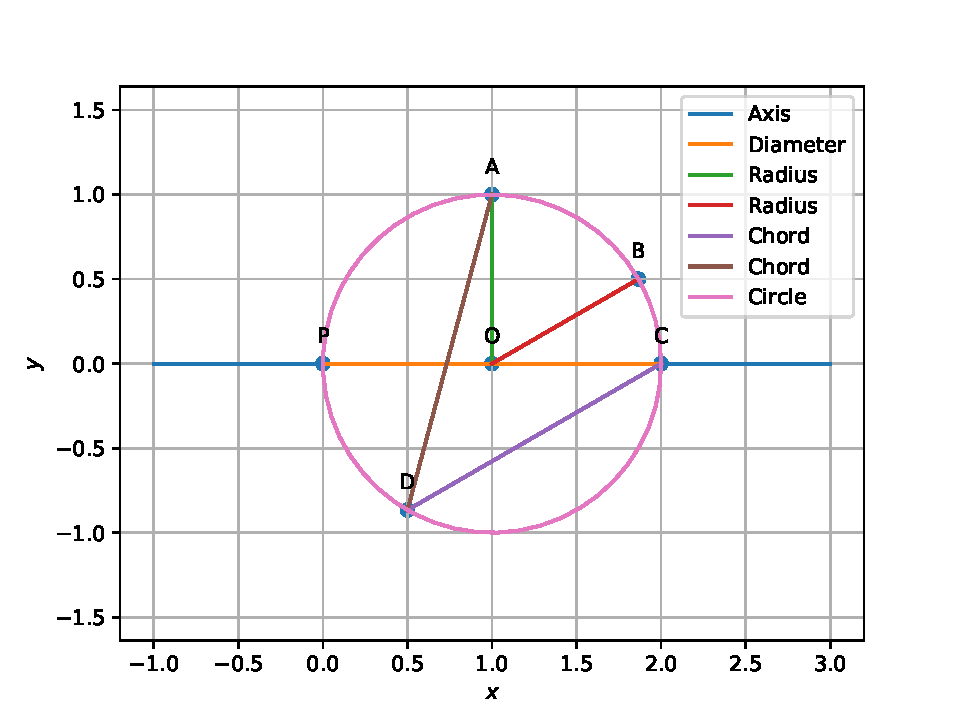
\includegraphics[width=\columnwidth]{chapters/9/10/5/1/figs/circle1.pdf}
\caption{}
\label{fig:chapters/9/10/5/1/Fig1}
\end{figure}
%
\begin{table}[h!]
	\centering
	%\subimport{../chapters/9/10/5/1/tables/}{table1.tex}
     %%%%%%%%%%%%%%%%%%%%%%%%%%%%%%%%%%%%%%%%%%%%%%%%%%%%%%%%%%%%%%%%%%%%%%
%%                                                                  %%
%%  This is the header of a LaTeX2e file exported from Gnumeric.    %%
%%                                                                  %%
%%  This file can be compiled as it stands or included in another   %%
%%  LaTeX document. The table is based on the longtable package so  %%
%%  the longtable options (headers, footers...) can be set in the   %%
%%  preamble section below (see PRAMBLE).                           %%
%%                                                                  %%
%%  To include the file in another, the following two lines must be %%
%%  in the including file:                                          %%
%%        \def\inputGnumericTable{}                                 %%
%%  at the beginning of the file and:                               %%
%%        \input{name-of-this-file.tex}                             %%
%%  where the table is to be placed. Note also that the including   %%
%%  file must use the following packages for the table to be        %%
%%  rendered correctly:                                             %%
%%    \usepackage[latin1]{inputenc}                                 %%
%%    \usepackage{color}                                            %%
%%    \usepackage{array}                                            %%
%%    \usepackage{longtable}                                        %%
%%    \usepackage{calc}                                             %%
%%    \usepackage{multirow}                                         %%
%%    \usepackage{hhline}                                           %%
%%    \usepackage{ifthen}                                           %%
%%  optionally (for landscape tables embedded in another document): %%
%%    \usepackage{lscape}                                           %%
%%                                                                  %%
%%%%%%%%%%%%%%%%%%%%%%%%%%%%%%%%%%%%%%%%%%%%%%%%%%%%%%%%%%%%%%%%%%%%%



%%  This section checks if we are begin input into another file or  %%
%%  the file will be compiled alone. First use a macro taken from   %%
%%  the TeXbook ex 7.7 (suggestion of Han-Wen Nienhuys).            %%
\def\ifundefined#1{\expandafter\ifx\csname#1\endcsname\relax}


%%  Check for the \def token for inputed files. If it is not        %%
%%  defined, the file will be processed as a standalone and the     %%
%%  preamble will be used.                                          %%
\ifundefined{inputGnumericTable}

%%  We must be able to close or not the document at the end.        %%
	\def\gnumericTableEnd{\end{document}}


%%%%%%%%%%%%%%%%%%%%%%%%%%%%%%%%%%%%%%%%%%%%%%%%%%%%%%%%%%%%%%%%%%%%%%
%%                                                                  %%
%%  This is the PREAMBLE. Change these values to get the right      %%
%%  paper size and other niceties.                                  %%
%%                                                                  %%
%%%%%%%%%%%%%%%%%%%%%%%%%%%%%%%%%%%%%%%%%%%%%%%%%%%%%%%%%%%%%%%%%%%%%%

	\documentclass[12pt%
			  %,landscape%
                    ]{report}
       \usepackage[latin1]{inputenc}
       \usepackage{fullpage}
       \usepackage{color}
       \usepackage{array}
       \usepackage{longtable}
       \usepackage{calc}
       \usepackage{multirow}
       \usepackage{hhline}
       \usepackage{ifthen}
       \usepackage{gensymb}
       \usepackage{graphicx}
\usepackage{amsmath}
\usepackage{mathtools}
\newcommand{\mydet}[1]{\ensuremath{\begin{vmatrix}#1\end{vmatrix}}}
\providecommand{\brak}[1]{\ensuremath{\left(#1\right)}}
\providecommand{\norm}[1]{\left\lVert#1\right\rVert}
\newcommand{\solution}{\noindent \textbf{Solution: }}
\newcommand{\myvec}[1]{\ensuremath{\begin{pmatrix}#1\end{pmatrix}}}
\let\vec\mathbf
	\begin{document}


%%  End of the preamble for the standalone. The next section is for %%
%%  documents which are included into other LaTeX2e files.          %%
\else

%%  We are not a stand alone document. For a regular table, we will %%
%%  have no preamble and only define the closing to mean nothing.   %%
    \def\gnumericTableEnd{}

%%  If we want landscape mode in an embedded document, comment out  %%
%%  the line above and uncomment the two below. The table will      %%
%%  begin on a new page and run in landscape mode.                  %%
%       \def\gnumericTableEnd{\end{landscape}}
%       \begin{landscape}


%%  End of the else clause for this file being \input.              %%
\fi

%%%%%%%%%%%%%%%%%%%%%%%%%%%%%%%%%%%%%%%%%%%%%%%%%%%%%%%%%%%%%%%%%%%%%%
%%                                                                  %%
%%  The rest is the gnumeric table, except for the closing          %%
%%  statement. Changes below will alter the table's appearance.     %%
%%                                                                  %%
%%%%%%%%%%%%%%%%%%%%%%%%%%%%%%%%%%%%%%%%%%%%%%%%%%%%%%%%%%%%%%%%%%%%%%
\providecommand{\gnumericmathit}[1]{#1} 
%%  Uncomment the next line if you would like your numbers to be in %%
%%  italics if they are italizised in the gnumeric table.           %%
%\renewcommand{\gnumericmathit}[1]{\mathit{#1}}
\providecommand{\gnumericPB}[1]%
{\let\gnumericTemp=\\#1\let\\=\gnumericTemp\hspace{0pt}}
 \ifundefined{gnumericTableWidthDefined}
        \newlength{\gnumericTableWidth}
        \newlength{\gnumericTableWidthComplete}
        \newlength{\gnumericMultiRowLength}
        \global\def\gnumericTableWidthDefined{}
 \fi
%% The following setting protects this code from babel shorthands.  %%
 \ifthenelse{\isundefined{\languageshorthands}}{}{\languageshorthands{english}}
%%  The default table format retains the relative column widths of  %%
%%  gnumeric. They can easily be changed to c, r or l. In that case %%
%%  you may want to comment out the next line and uncomment the one %%
%%  thereafter                                                      %%
\providecommand\gnumbox{\makebox[0pt]}
%%\providecommand\gnumbox[1][]{\makebox}

%% to adjust positions in multirow situations                       %%
\setlength{\bigstrutjot}{\jot}
\setlength{\extrarowheight}{\doublerulesep}

%%  The \setlongtables command keeps column widths the same across  %%
%%  pages. Simply comment out next line for varying column widths.  %%
\setlongtables

\setlength\gnumericTableWidth{%
	40pt+%
	35pt+%
	210pt+%
0pt}
\def\gumericNumCols{3}
\setlength\gnumericTableWidthComplete{\gnumericTableWidth+%
         \tabcolsep*\gumericNumCols*2+\arrayrulewidth*\gumericNumCols}
\ifthenelse{\lengthtest{\gnumericTableWidthComplete > \linewidth}}%
         {\def\gnumericScale{\ratio{\linewidth-%
                        \tabcolsep*\gumericNumCols*2-%
                        \arrayrulewidth*\gumericNumCols}%
{\gnumericTableWidth}}}%
{\def\gnumericScale{1}}

%%%%%%%%%%%%%%%%%%%%%%%%%%%%%%%%%%%%%%%%%%%%%%%%%%%%%%%%%%%%%%%%%%%%%%
%%                                                                  %%
%% The following are the widths of the various columns. We are      %%
%% defining them here because then they are easier to change.       %%
%% Depending on the cell formats we may use them more than once.    %%
%%                                                                  %%
%%%%%%%%%%%%%%%%%%%%%%%%%%%%%%%%%%%%%%%%%%%%%%%%%%%%%%%%%%%%%%%%%%%%%%

\ifthenelse{\isundefined{\gnumericColA}}{\newlength{\gnumericColA}}{}\settowidth{\gnumericColA}{\begin{tabular}{@{}p{40pt*\gnumericScale}@{}}x\end{tabular}}
\ifthenelse{\isundefined{\gnumericColB}}{\newlength{\gnumericColB}}{}\settowidth{\gnumericColB}{\begin{tabular}{@{}p{35pt*\gnumericScale}@{}}x\end{tabular}}
\ifthenelse{\isundefined{\gnumericColC}}{\newlength{\gnumericColC}}{}\settowidth{\gnumericColC}{\begin{tabular}{@{}p{210pt*\gnumericScale}@{}}x\end{tabular}}

\begin{longtable}[c]{%
	b{\gnumericColA}%
	b{\gnumericColB}%
	b{\gnumericColC}%
	}

%%%%%%%%%%%%%%%%%%%%%%%%%%%%%%%%%%%%%%%%%%%%%%%%%%%%%%%%%%%%%%%%%%%%%%
%%  The longtable options. (Caption, headers... see Goosens, p.124) %%
%	\caption{The Table Caption.}             \\	%
% \hline	% Across the top of the table.
%%  The rest of these options are table rows which are placed on    %%
%%  the first, last or every page. Use \multicolumn if you want.    %%

%%  Header for the first page.                                      %%
%	\multicolumn{3}{c}{The First Header} \\ \hline 
%	\multicolumn{1}{c}{colTag}	%Column 1
%	&\multicolumn{1}{c}{colTag}	%Column 2
%	&\multicolumn{1}{c}{colTag}	\\ \hline %Last column
%	\endfirsthead

%%  The running header definition.                                  %%
%	\hline
%	\multicolumn{3}{l}{\ldots\small\slshape continued} \\ \hline
%	\multicolumn{1}{c}{colTag}	%Column 1
%	&\multicolumn{1}{c}{colTag}	%Column 2
%	&\multicolumn{1}{c}{colTag}	\\ \hline %Last column
%	\endhead

%%  The running footer definition.                                  %%
%	\hline
%	\multicolumn{3}{r}{\small\slshape continued\ldots} \\
%	\endfoot

%%  The ending footer definition.                                   %%
%	\multicolumn{3}{c}{That's all folks} \\ \hline 
%	\endlastfoot
%%%%%%%%%%%%%%%%%%%%%%%%%%%%%%%%%%%%%%%%%%%%%%%%%%%%%%%%%%%%%%%%%%%%%%

\hhline{|-|-|-}
	 \multicolumn{1}{|p{\gnumericColA}|}%
	{\gnumericPB{\raggedright}\gnumbox[l]{\textbf{Symbol}}}
	&\multicolumn{1}{p{\gnumericColB}|}%
	{\gnumericPB{\raggedright}\gnumbox[l]{\textbf{Values}}}
	&\multicolumn{1}{p{\gnumericColC}|}%
	{\gnumericPB{\raggedright}\gnumbox[l]{\textbf{Description}}}
\\
\hhline{|---|}
	 \multicolumn{1}{|p{\gnumericColA}|}%
	{\gnumericPB{\raggedright}\gnumbox[l]{r}}
	&\multicolumn{1}{p{\gnumericColB}|}%
	{\gnumericPB{\raggedright}\gnumbox[l]{1 unit}}
	&\multicolumn{1}{p{\gnumericColC}|}%
	{\gnumericPB{\raggedright}\gnumbox[l]{Radius of OA and OB}}
\\
\hhline{|---|}
	 \multicolumn{1}{|p{\gnumericColA}|}%
	{\gnumericPB{\raggedright}\gnumbox[l]{$\vec{O}$}}
	&\multicolumn{1}{p{\gnumericColB}|}%
	{\gnumericPB{\raggedright}\gnumbox[l]{\myvec{0\\0}}}
	&\multicolumn{1}{p{\gnumericColC}|}%
	{\gnumericPB{\raggedright}\gnumbox[l]{Center of the circle }}
\\
\hhline{|---|}
	 \multicolumn{1}{|p{\gnumericColA}|}%
	{\gnumericPB{\raggedright}\gnumbox[l]{$\vec{C}$}}
	&\multicolumn{1}{p{\gnumericColB}|}%
	{\gnumericPB{\raggedright}\gnumbox[l]{\myvec{1\\0}}}
	&\multicolumn{1}{p{\gnumericColC}|}%
	{\gnumericPB{\raggedright}\gnumbox[l]{Standard basis vector $\vec{e}_1$}}
\\
\hhline{|---|}
	 \multicolumn{1}{|p{\gnumericColA}|}%
	{\gnumericPB{\raggedright}\gnumbox[l]{$\alpha$}}
	&\multicolumn{1}{p{\gnumericColB}|}%
	{\gnumericPB{\raggedright}\gnumbox[l]{30\degree}}
	&\multicolumn{1}{p{\gnumericColC}|}%
	{\gnumericPB{\raggedright}\gnumbox[l]{$\angle$BOC}}
\\
\hhline{|---|}
	 \multicolumn{1}{|p{\gnumericColA}|}%
	{\gnumericPB{\raggedright}\gnumbox[l]{$\beta$}}
	&\multicolumn{1}{p{\gnumericColB}|}%
	{\gnumericPB{\raggedright}\gnumbox[l]{60\degree}}
	&\multicolumn{1}{p{\gnumericColC}|}%
	{\gnumericPB{\raggedright}\gnumbox[l]{$\angle$AOB}}
\\
\hhline{|---|}
	 \multicolumn{1}{|p{\gnumericColA}|}%
	{\gnumericPB{\raggedright}\gnumbox[l]{\textbf{$\gamma$}}}
	&\multicolumn{1}{p{\gnumericColB}|}%
	{\gnumericPB{\raggedright}\gnumbox[l]{??}}
	&\multicolumn{1}{p{\gnumericColC}|}%
	{\gnumericPB{\raggedright}\gnumbox[l]{$\angle$ADC}}
\\
\hhline{|-|-|-|}
\end{longtable}

\ifthenelse{\isundefined{\languageshorthands}}{}{\languageshorthands{\languagename}}
\gnumericTableEnd%

%	\caption{}
	\label{table:chapters/9/10/5/1/table1}
	\end{table}
The input parameters are available in Table
	\ref{table:chapters/9/10/5/1/table1} yielding
\begin{align}
	\vec{C} =\vec{e}_1= \myvec{1\\0},\,
	\vec{A} = \myvec{\cos(\alpha+\beta)\\\sin(\alpha+\beta)},\,
	\vec{D} = \myvec{\cos\gamma\\\sin\gamma}.
\end{align}
Since
\begin{align}
	 \vec{A-D}& = \myvec{\cos(\alpha+\beta) - \cos\gamma\\\sin(\alpha+\beta) - \sin\gamma},
	 \vec{C-D} &= \myvec{1 - \cos\gamma\\-\sin\gamma},
	 \norm{\vec{A-D}}\norm{\vec{C-D}}& = 4 \sin\frac{\alpha+\gamma}2\sin\frac{\beta+\gamma}2,
	 \\
	\cos(\angle ADC) &= \frac{\vec{(A-D)^\top(C-D)}}{\norm{\vec{A-D}}\norm{\vec{C-D}}},
	\label{eq:2}
	\\
	&= 4\sin\frac{\alpha+\gamma}2\sin\frac{\beta+\gamma}2\cos\frac{\alpha+\beta}2
 = \cos\frac{\alpha+\beta}{2}
	\label{eq:7}
\end{align}
Substituting $\alpha$ and $\beta$ in \eqref{eq:7}
\begin{align}
\angle ADC = \frac{\alpha+\beta}{2}=\frac{(30\degree + 60\degree )}{2}=45\degree
\end{align}
See Fig. 
\ref{fig:chapters/9/10/5/1/Fig1}.



\item A chord of a circle is equal to the radius of the circle. Find the angle subtended by the chord at a point on the minor arc and also at a point on the major arc.
\label{chapters/9/10/5/2}
\\
\solution
\documentclass[12pt]{article}
\usepackage{graphicx}
\usepackage{amsmath}
\usepackage{mathtools}
\usepackage{gensymb}
\usepackage[latin1]{inputenc}
\usepackage{fullpage}
\usepackage{color}
\usepackage{array}
\usepackage{longtable}
\usepackage{calc}
\usepackage{multirow}
\usepackage{hhline}
\usepackage{ifthen}
\usepackage{booktabs}
\usepackage{graphicx}
\def\inputGnumericTable{}

\newcommand{\mydet}[1]{\ensuremath{\begin{vmatrix}#1\end{vmatrix}}}
\providecommand{\brak}[1]{\ensuremath{\left(#1\right)}}
\providecommand{\norm}[1]{\left\lVert#1\right\rVert}
\newcommand{\solution}{\noindent \textbf{Solution: }}
\newcommand{\myvec}[1]{\ensuremath{\begin{pmatrix}#1\end{pmatrix}}}
\let\vec\mathbf

\begin{document}
\begin{center}
\textbf\large{CHAPTER-9 \\ CIRCLES}

\end{center}
\begin{enumerate}
\section{EXERCISE-10.5}
\item A chord of a circle is equal to the radius of the circle. Find the angle subtended by the chord at a point on the minor arc and also at a point on the major arc.
\section{SOLUTION}
The input parameters are\\
\begin{table}[h!]
	%%%%%%%%%%%%%%%%%%%%%%%%%%%%%%%%%%%%%%%%%%%%%%%%%%%%%%%%%%%%%%%%%%%%%%
%%                                                                  %%
%%  This is the header of a LaTeX2e file exported from Gnumeric.    %%
%%                                                                  %%
%%  This file can be compiled as it stands or included in another   %%
%%  LaTeX document. The table is based on the longtable package so  %%
%%  the longtable options (headers, footers...) can be set in the   %%
%%  preamble section below (see PRAMBLE).                           %%
%%                                                                  %%
%%  To include the file in another, the following two lines must be %%
%%  in the including file:                                          %%
%%        \def\inputGnumericTable{}                                 %%
%%  at the beginning of the file and:                               %%
%%        \input{name-of-this-file.tex}                             %%
%%  where the table is to be placed. Note also that the including   %%
%%  file must use the following packages for the table to be        %%
%%  rendered correctly:                                             %%
%%    \usepackage[latin1]{inputenc}                                 %%
%%    \usepackage{color}                                            %%
%%    \usepackage{array}                                            %%
%%    \usepackage{longtable}                                        %%
%%    \usepackage{calc}                                             %%
%%    \usepackage{multirow}                                         %%
%%    \usepackage{hhline}                                           %%
%%    \usepackage{ifthen}                                           %%
%%  optionally (for landscape tables embedded in another document): %%
%%    \usepackage{lscape}                                           %%
%%                                                                  %%
%%%%%%%%%%%%%%%%%%%%%%%%%%%%%%%%%%%%%%%%%%%%%%%%%%%%%%%%%%%%%%%%%%%%%%



%%  This section checks if we are begin input into another file or  %%
%%  the file will be compiled alone. First use a macro taken from   %%
%%  the TeXbook ex 7.7 (suggestion of Han-Wen Nienhuys).            %%
\def\ifundefined#1{\expandafter\ifx\csname#1\endcsname\relax}


%%  Check for the \def token for inputed files. If it is not        %%
%%  defined, the file will be processed as a standalone and the     %%
%%  preamble will be used.                                          %%
\ifundefined{inputGnumericTable}

%%  We must be able to close or not the document at the end.        %%
	\def\gnumericTableEnd{\end{document}}


%%%%%%%%%%%%%%%%%%%%%%%%%%%%%%%%%%%%%%%%%%%%%%%%%%%%%%%%%%%%%%%%%%%%%%
%%                                                                  %%
%%  This is the PREAMBLE. Change these values to get the right      %%
%%  paper size and other niceties.                                  %%
%%                                                                  %%
%%%%%%%%%%%%%%%%%%%%%%%%%%%%%%%%%%%%%%%%%%%%%%%%%%%%%%%%%%%%%%%%%%%%%%

	\documentclass[12pt%
			  %,landscape%
                    ]{report}
       \usepackage[latin1]{inputenc}
       \usepackage{fullpage}
       \usepackage{color}
       \usepackage{array}
       \usepackage{longtable}
       \usepackage{calc}
       \usepackage{multirow}
       \usepackage{hhline}
       \usepackage{ifthen}

	\begin{document}


%%  End of the preamble for the standalone. The next section is for %%
%%  documents which are included into other LaTeX2e files.          %%
\else

%%  We are not a stand alone document. For a regular table, we will %%
%%  have no preamble and only define the closing to mean nothing.   %%
    \def\gnumericTableEnd{}

%%  If we want landscape mode in an embedded document, comment out  %%
%%  the line above and uncomment the two below. The table will      %%
%%  begin on a new page and run in landscape mode.                  %%
%       \def\gnumericTableEnd{\end{landscape}}
%       \begin{landscape}


%%  End of the else clause for this file being \input.              %%
\fi

%%%%%%%%%%%%%%%%%%%%%%%%%%%%%%%%%%%%%%%%%%%%%%%%%%%%%%%%%%%%%%%%%%%%%%
%%                                                                  %%
%%  The rest is the gnumeric table, except for the closing          %%
%%  statement. Changes below will alter the table's appearance.     %%
%%                                                                  %%
%%%%%%%%%%%%%%%%%%%%%%%%%%%%%%%%%%%%%%%%%%%%%%%%%%%%%%%%%%%%%%%%%%%%%%

\providecommand{\gnumericmathit}[1]{#1} 
%%  Uncomment the next line if you would like your numbers to be in %%
%%  italics if they are italizised in the gnumeric table.           %%
%\renewcommand{\gnumericmathit}[1]{\mathit{#1}}
\providecommand{\gnumericPB}[1]%
{\let\gnumericTemp=\\#1\let\\=\gnumericTemp\hspace{0pt}}
 \ifundefined{gnumericTableWidthDefined}
        \newlength{\gnumericTableWidth}
        \newlength{\gnumericTableWidthComplete}
        \newlength{\gnumericMultiRowLength}
        \global\def\gnumericTableWidthDefined{}
 \fi
%% The following setting protects this code from babel shorthands.  %%
 \ifthenelse{\isundefined{\languageshorthands}}{}{\languageshorthands{english}}
%%  The default table format retains the relative column widths of  %%
%%  gnumeric. They can easily be changed to c, r or l. In that case %%
%%  you may want to comment out the next line and uncomment the one %%
%%  thereafter                                                      %%
\providecommand\gnumbox{\makebox[0pt]}
%%\providecommand\gnumbox[1][]{\makebox}

%% to adjust positions in multirow situations                       %%
\setlength{\bigstrutjot}{\jot}
\setlength{\extrarowheight}{\doublerulesep}

%%  The \setlongtables command keeps column widths the same across  %%
%%  pages. Simply comment out next line for varying column widths.  %%
\setlongtables

\setlength\gnumericTableWidth{%
	53pt+%
	53pt+%
	82pt+%
	53pt+%
0pt}
\def\gumericNumCols{4}
\setlength\gnumericTableWidthComplete{\gnumericTableWidth+%
         \tabcolsep*\gumericNumCols*2+\arrayrulewidth*\gumericNumCols}
\ifthenelse{\lengthtest{\gnumericTableWidthComplete > \linewidth}}%
         {\def\gnumericScale{1*\ratio{\linewidth-%
                        \tabcolsep*\gumericNumCols*2-%
                        \arrayrulewidth*\gumericNumCols}%
{\gnumericTableWidth}}}%
{\def\gnumericScale{1}}

%%%%%%%%%%%%%%%%%%%%%%%%%%%%%%%%%%%%%%%%%%%%%%%%%%%%%%%%%%%%%%%%%%%%%%
%%                                                                  %%
%% The following are the widths of the various columns. We are      %%
%% defining them here because then they are easier to change.       %%
%% Depending on the cell formats we may use them more than once.    %%
%%                                                                  %%
%%%%%%%%%%%%%%%%%%%%%%%%%%%%%%%%%%%%%%%%%%%%%%%%%%%%%%%%%%%%%%%%%%%%%%

\ifthenelse{\isundefined{\gnumericColA}}{\newlength{\gnumericColA}}{}\settowidth{\gnumericColA}{\begin{tabular}{@{}p{53pt*\gnumericScale}@{}}x\end{tabular}}
\ifthenelse{\isundefined{\gnumericColB}}{\newlength{\gnumericColB}}{}\settowidth{\gnumericColB}{\begin{tabular}{@{}p{53pt*\gnumericScale}@{}}x\end{tabular}}
\ifthenelse{\isundefined{\gnumericColC}}{\newlength{\gnumericColC}}{}\settowidth{\gnumericColC}{\begin{tabular}{@{}p{82pt*\gnumericScale}@{}}x\end{tabular}}
\ifthenelse{\isundefined{\gnumericColD}}{\newlength{\gnumericColD}}{}\settowidth{\gnumericColD}{\begin{tabular}{@{}p{53pt*\gnumericScale}@{}}x\end{tabular}}

	\begin{center}
\begin{tabular}[c]{%
	b{\gnumericColA}%
	b{\gnumericColB}%
	b{\gnumericColC}%
	b{\gnumericColD}%
	}

%%%%%%%%%%%%%%%%%%%%%%%%%%%%%%%%%%%%%%%%%%%%%%%%%%%%%%%%%%%%%%%%%%%%%%
%%  The longtable options. (Caption, headers... see Goosens, p.124) %%
%	\caption{The Table Caption.}             \\	%
% \hline	% Across the top of the table.
%%  The rest of these options are table rows which are placed on    %%
%%  the first, last or every page. Use \multicolumn if you want.    %%

%%  Header for the first page.                                      %%
%	\multicolumn{4}{c}{The First Header} \\ \hline 
%	\multicolumn{1}{c}{colTag}	%Column 1
%	&\multicolumn{1}{c}{colTag}	%Column 2
%	&\multicolumn{1}{c}{colTag}	%Column 3
%	&\multicolumn{1}{c}{colTag}	\\ \hline %Last column
%	\endfirsthead

%%  The running header definition.                                  %%
%	\hline
%	\multicolumn{4}{l}{\ldots\small\slshape continued} \\ \hline
%	\multicolumn{1}{c}{colTag}	%Column 1
%	&\multicolumn{1}{c}{colTag}	%Column 2
%	&\multicolumn{1}{c}{colTag}	%Column 3
%	&\multicolumn{1}{c}{colTag}	\\ \hline %Last column
%	\endhead

%%  The running footer definition.                                  %%
%	\hline
%	\multicolumn{4}{r}{\small\slshape continued\ldots} \\
%	\endfoot

%%  The ending footer definition.                                   %%
%	\multicolumn{4}{c}{That's all folks} \\ \hline 
%	\endlastfoot
%%%%%%%%%%%%%%%%%%%%%%%%%%%%%%%%%%%%%%%%%%%%%%%%%%%%%%%%%%%%%%%%%%%%%%

\hhline{|-|-|-~}
	 \multicolumn{1}{|p{\gnumericColA}|}%
	{\gnumericPB{\centering}\gnumbox{\textbf{Symbol}}}
	&\multicolumn{1}{p{\gnumericColB}|}%
	{\gnumericPB{\centering}\gnumbox{\textbf{Value}}}
	&\multicolumn{1}{p{\gnumericColC}|}%
	{\gnumericPB{\centering}\gnumbox{\textbf{Description}}}
	&
\\
\hhline{|---|~}
	 \multicolumn{1}{|p{\gnumericColA}|}%
	{\gnumericPB{\centering}\gnumbox{$\vec{P}$}}
	&\multicolumn{1}{p{\gnumericColB}|}%
	{\gnumericPB{\centering}\gnumbox{$\myvec{5\\-3}$}}
	&\multicolumn{1}{p{\gnumericColC}|}%
	{\gnumericPB{\centering}\gnumbox{First point}}
	&
\\
\hhline{|---|~}
	 \multicolumn{1}{|p{\gnumericColA}|}%
	{\gnumericPB{\centering}\gnumbox{$\vec{Q}$}}
	&\multicolumn{1}{p{\gnumericColB}|}%
	{\gnumericPB{\centering}\gnumbox{$\myvec{0\\1}$}}
	&\multicolumn{1}{p{\gnumericColC}|}%
	{\gnumericPB{\centering}\gnumbox{Second point}}
	&
\\
\hhline{|---|~}
	 \multicolumn{1}{|p{\gnumericColA}|}%
	{\gnumericPB{\centering}\gnumbox{$\vec{R}$}}
	&\multicolumn{1}{p{\gnumericColB}|}%
	{\gnumericPB{\centering}\gnumbox{$\myvec{?\\6}$}}
	&\multicolumn{1}{p{\gnumericColC}|}%
	{\gnumericPB{\centering}\gnumbox{Desired point}}
	&
\\
\hhline{|-|-|-|~}
\end{tabular}
	\end{center}

\ifthenelse{\isundefined{\languageshorthands}}{}{\languageshorthands{\languagename}}
\gnumericTableEnd
\caption{}
\label{table}	
\end{table}
\\
Take three points Q,R and P on a unit circle  at angles $\theta,\alpha,\text{ and }\beta$.Then
\begin{align}
	\vec{Q} = \myvec{\cos\theta\\ \sin\theta},
	\vec{R} = \myvec{\cos\alpha\\ \sin\alpha},
	\vec{S} = \myvec{\cos\beta\\ \sin\beta}
\end{align}
\begin{align}
	\cos\angle QRP&= \frac{\brak{\vec{Q}-\vec{R}}\brak{\vec{P}-\vec{R}}}{\norm{\vec{Q}-\vec{R}}\norm{\vec{P}-\vec{R}}}\label{eq:2}
\end{align}
Where
\begin{align}
\brak{\vec{Q}-\vec{R}}\brak{\vec{P}-\vec{R}}&= \brak{\cos\theta-\cos\alpha}\brak{ \sin\theta-\sin\alpha}\brak{1-\cos\alpha}\brak{0-\sin\alpha}\\
&=\brak{\cos\theta-\cos\alpha}\cos\alpha+\brak{\sin\theta-\sin\alpha}\\
&=2\sin\frac{\theta-\alpha}{2}\sin\frac{\theta+\alpha}{2}\cos\alpha+2\cos\frac{\theta+\alpha}{2}\sin\frac{\theta-\alpha}{2}\\
&=\brak{\cos\alpha-\cos\theta}\cos\alpha+\brak{\sin\theta-\sin\alpha}\label{eq:6}
\end{align}
\begin{align}
\norm{\vec{Q}-\vec{R}}^2\norm{\vec{P}-\vec{R}}^2 &= \brak{\cos\theta-\cos\alpha}^2+\brak{\sin\theta-\sin\alpha}^2
	\brak{1-\cos\alpha}^2+\brak{0-\sin\alpha}^2\\
	&=\brak{2-2\cos\theta\cos\alpha-2\sin\theta\sin\alpha}\brak{2-\cos\alpha}\label{eq:8}
\end{align}
substituing the \eqref{eq:6} and \eqref{eq:8} in \eqref{eq:2}
\begin{align}
\cos\angle QRP&=\frac{2.079}{4.323}\\
\angle QRP&=\cos^{-1}0.480\\
\angle QRP&=62\degree
\end{align}
\begin{align}
\cos\angle QSP&= \frac{\brak{\vec{Q}-\vec{S}}\brak{\vec{P}-\vec{S}}}{\norm{\vec{Q}-\vec{S}}\norm{\vec{P}-\vec{S}}}\label{eq:12}
\end{align}
\begin{align}
\brak{\vec{Q}-\vec{S}}\brak{\vec{P}-\vec{S}}&= \brak{\cos\theta-\cos\beta}\brak{\sin\theta-\sin\beta}\brak{1-\cos\beta}\brak{0-\sin\beta}\\
&=\brak{\cos\theta-\cos\beta}\cos\beta+\brak{\sin\theta-\sin\beta}\\
&=2\sin\frac{\theta-\beta}{2}\sin\frac{\theta+\beta}{2}\cos\beta+2\cos\frac{\theta+\beta}{2}\sin\frac{\theta-\beta}{2}\\
&=\brak{\cos\beta-\cos\theta}\cos\beta+\brak{\sin\theta-\sin\beta}\label{eq:16}
\end{align}
\begin{align}
\norm{\vec{Q}-\vec{S}}^2\norm{\vec{P}-\vec{S}}^2 &= \brak{\cos\theta-\cos\beta}^2+\brak{\sin\theta-\sin\beta}^2
	\brak{1-\cos\beta}^2+\brak{0-\sin\beta}^2\\
	&=\brak{2-2\cos\theta\cos\beta-2\sin\theta\sin\beta}\brak{2-\cos\beta}\label{eq:18}
\end{align}
substituing the \eqref{eq:16} and \eqref{eq:18} in \eqref{eq:12}
\begin{align}
\cos\angle QSP&=\frac{1.048}{1.098}\\
\angle QSP&=\cos^{-1}0.954\\
\angle QSP&=17\degree
\end{align}
\section{FIGURE}
\begin{figure}[h]
\centering
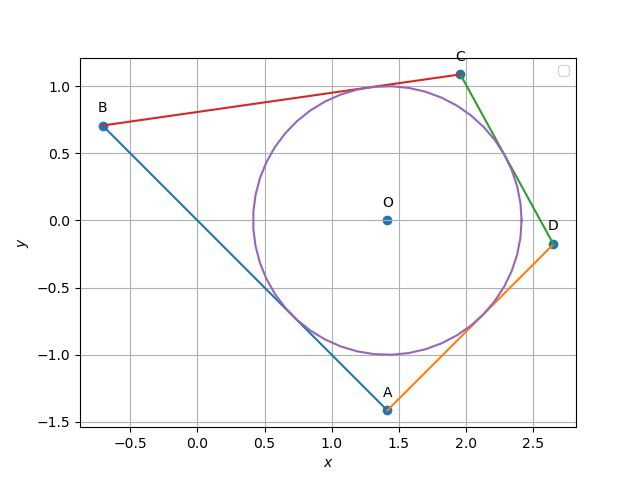
\includegraphics[width=\columnwidth]{circle.png}
\caption{}
		\label{fig:Figure}
\end{figure}
\end{enumerate}
\end{document}

\item 
\label{chapters/9/10/5/3}
\iffalse
\documentclass[journal,10pt,twocolumn]{article}
\usepackage{graphicx, float}
\usepackage[margin=0.5in]{geometry}
\usepackage{amsmath, bm}
\usepackage{array}
\usepackage{booktabs}


\providecommand{\norm}[1]{\left\lVert#1\right\rVert}
\let\vec\mathbf
\newcommand{\myvec}[1]{\ensuremath{\begin{pmatrix}#1\end{pmatrix}}}
\newcommand{\mydet}[1]{\ensuremath{\begin{vmatrix}#1\end{vmatrix}}}

\title{\textbf{Circle Assignment}}
\author{Maddu Dinesh}
\date{September 2022}

\begin{document}

\maketitle
\paragraph{\textit{Problem Statement} -
\fi
Let $\angle PQR = 100\degree$ where $\vec{P}\vec{Q}, \vec{R}$ are points on a circle with centre $\vec{O}$. Find $\angle OPR$.
	\begin{figure}[!ht]
		\centering
 \includegraphics[width=\columnwidth]{chapters/9/10/5/3/figs/fig-1.pdf}
		\caption{}
		\label{fig:9/10/5/3}
  	\end{figure}
	\solution In Fig. 
		\ref{fig:9/10/5/3},
\begin{align}
	\vec{P} = \myvec{\cos\brak{\theta + 160} \\ \sin \brak{\theta + 160}}, \vec{Q} = \myvec{\cos \alpha\\ \sin \alpha}, \vec{R} = \myvec{\cos \theta \\ \sin \theta}.
\end{align}

\iffalse

\section*{\large Solution}

\begin{figure}[H]
\centering
\includegraphics[width=1\columnwidth]{fig-1.pdf}
\label{fig:triangle}
\end{figure}



Given  $\angle$PQR=100°





\section*{ Construction}






{
\setlength\extrarowheight{1pt}


\begin{tabular}{|c|c|c|}
 \hline
 \textbf{Symbol}&\textbf{Value}&\textbf{Description}\\
 \hline
 O&&Centre\\
 \hline
 $\angle$PQR&100$^\circ$&Angle between vectors P and R\\
 \hline
 $\angle$OPR&??&Angle b/w vectors O and R w.r.to P\\
 \hline
 
\end{tabular}

{


\section*{Proof:}
From assumptions the vector points P,Q,R be
\begin{eqnarray}
 \vec{P} = \myvec{cos\theta_1\\sin\theta_1},
 \vec{Q} = \myvec{cos\theta_2\\sin\theta_2},
 \vec{R} = \myvec{cos\theta_3\\sin\theta_3},
 \vec{O} = \myvec{0\\0}
\end{eqnarray}

\begin{align}
 cos(\angle PQR) = \frac{(P-Q)^T(R-Q)}{\norm{P-Q}\norm{R-Q}}
 \label{pf2-eq-1}
\end{align}

Where
 \begin{eqnarray}
 \vec{P-Q} = \myvec{cos\theta_1 - cos\theta_2\\sin\theta_1 - sin\theta_2},
 \vec{R-Q} = \myvec{cos\theta_3 - cos\theta_2\\sin\theta_3 - sin\theta_2}
\end{eqnarray}
 

\begin{eqnarray*}
 (P-Q)^T(R-Q)=\myvec{cos\theta_1 - cos\theta_2  sin\theta_1 - sin\theta_2}
 \myvec{cos\theta_3 - cos\theta_2\\sin\theta_3 - sin\theta_2}
\end{eqnarray*}

\begin{multline*}
 = (\cos\theta_1-\cos\theta_2)(\cos\theta_3-\cos\theta_2)+(\sin\theta_1-\sin\theta_2)(\sin\theta_3-\sin\theta_2)
\end{multline*}

\begin{multline*}
 = -2\sin\frac{\theta_1-\theta_2}2\sin\frac{\theta_1+\theta_2}2 \cdot(-2)\sin\frac{\theta_3-\theta_2}2\sin\frac{\theta_3+\theta_2}2 \\\quad+ 2\cos\frac{\theta_1+\theta_2}2\sin\frac{\theta_1-\theta_2}2 \cdot 2\cos\frac{\theta_2+\theta_3}2\sin\frac{\theta_3-\theta_2}2
\end{multline*}
\begin{multline*}
 = 4\sin\frac{\theta_1-\theta_2}2\sin\frac{\theta_3-\theta_2}2(\sin\frac{\theta_1+\theta_2}2\sin\frac{\theta_3+\theta_2}2+\\
 \cos\frac{\theta_1+\theta_2}2\cos\frac{\theta_3+\theta_2}2)
\end{multline*}
\begin{align*}
 = 4\sin\frac{\theta_1-\theta_2}2\sin\frac{\theta_3-\theta_2}2\cos\left(\frac{\theta_1+\theta_2}2-\frac{\theta_3+\theta_2}2\right)
\end{align*}
\begin{align}
 = 4\sin\frac{\theta_1-\theta_2}2\sin\frac{\theta_3-\theta_2}2\cos\frac{\theta_1-\theta_3}2
 \label{pf2-eq-2}
\end{align}

\begin{multline*}
 \norm{P-Q}^2\norm{R-Q}^2 = ((\cos\theta_1-\cos\theta_2)^2+(\sin\theta_1-\sin\theta_2)^2)\\
 ((\cos\theta_3-\cos\theta_2)^2+(\sin\theta_3-\sin\theta_2)^2)
\end{multline*}
\begin{multline*}
 = (2-2\cos\theta_1\cos\theta_2 - 2\sin\theta_1\sin\theta_2)(2-\\
 2\cos\theta_3\cos\theta_2 - 2\sin\theta_3\sin\theta_2)
\end{multline*}
\begin{align*}
 &= 16 \sin^2\frac{\theta_1-\theta_2}2\sin^2\frac{\theta_3-\theta_2}2
\end{align*}
\begin{align}
 \norm{P-Q}\norm{R-Q} = 4 \sin\frac{\theta_1-\theta_2}2\sin\frac{\theta_3-\theta_2}2
 \label{pf2-eq-3}
\end{align}

Substituting (\ref{pf2-eq-2}) and (\ref{pf2-eq-3}) in (\ref{pf2-eq-1}),
\begin{multline*}
 cos(\angle PQR) = \frac{4sin\frac{\theta_1-\theta_2}{2}sin\frac{\theta_3-\theta_2}{2}cos\frac{\theta_1-\theta_3}{2}}{4 \sin\frac{\theta_1-\theta_2}2\sin\frac{\theta_3-\theta_2}2}
\end{multline*}
\begin{equation}
cos(\angle PQR) = cos\frac{\theta_1-\theta_3}{2}
\label{pf2-eq-4}
\end{equation}
\begin{equation*}
\angle PQR = =\frac{\theta_1 - \theta_3 }{2}=100^\circ
\end{equation*}


\begin{align}
 cos(\angle OPR) = \frac{(P-R)^T(P-O)}{\norm{P-R}\norm{P-O}}
 \label{pf2-eq-5}
\end{align}

\begin{eqnarray}
 \vec{P-R} = \myvec{cos\theta_1 - cos\theta_3\\sin\theta_1 - sin\theta_3},
 \vec{P-O} = \myvec{cos\theta_1 \\sin\theta_1 }
\end{eqnarray}
 

\begin{eqnarray*}
 (P-R)^T(P-O)=\myvec{cos\theta_1 - cos\theta_3\\sin\theta_1 - sin\theta_3}
 \myvec{cos\theta_1 sin\theta_1 }
\end{eqnarray*}

\begin{multline*}
 = (\cos\theta_1-\cos\theta_3)(\cos\theta_1)+(\sin\theta_1-\sin\theta_3)(\sin\theta_1)
\end{multline*}
\begin{multline*}
 = (\cos^2{\theta_1}-\cos\theta_3\cos\theta_1)+(\sin^2{\theta_1}-\sin\theta_1\sin\theta_3)
\end{multline*}
\begin{align*}
 = 1-(\cos\theta_3\cos\theta_1+\sin\theta_1\sin\theta_3)
\end{align*}
\begin{equation}
=1-(cos(\theta_3-\theta_1))
\end{equation}
\begin{multline*}
 \norm{P-R}^2\norm{P-O}^2 = ((\cos\theta_1-\cos\theta_3)^2+(\sin\theta_1-\sin\theta_3)^2)\\
 ((\cos\theta_1)^2+(\sin\theta_1)^2)
\end{multline*}
\begin{align*}
 = 2-2\cos\theta_1\cos\theta_3-2\sin\theta_1\sin\theta_3
\end{align*}
\begin{align*}
 = 2(1-\cos(\theta_1-\theta_3) )
\end{align*}
\begin{align}
 \norm{P-R}\norm{P-O} = \sqrt{2(1-\cos(\theta_1-\theta_3))}
 \label{pf2-eq-6}
\end{align}
\begin{align*}
 cos(\angle OPR) = \frac{(1-\cos(\theta_1-\theta_3)) }{\sqrt{2(1-\cos(\theta_1-\theta_3))}}
\end{align*}
\begin{align*}
\cos(\angle OPR)=0.98
\end{align*}
\begin{align}
\angle OPR=10^\circ
\end{align}






\end{document}
Footer
\fi

\item If circles are drawn taking two sides of a triangle as diameters, prove that the point of intersection of these circles lie on the third side.
\label{chapters/9/10/5/10}
\\
\solution
\iffalse
\documentclass[journal,12pt,twocolumn]{IEEEtran}
\usepackage{setspace}
\usepackage{gensymb}
\singlespacing
\usepackage[cmex10]{amsmath}
\usepackage{amsthm}
\usepackage{mathrsfs}
\usepackage{txfonts}
\usepackage{stfloats}
\usepackage{bm}
\usepackage{cite}
\usepackage{cases}
\usepackage{subfig}
\usepackage{longtable}
\usepackage{multirow}
\usepackage{enumitem}
\usepackage{mathtools}
\usepackage{steinmetz}
\usepackage{tikz}
\usepackage{circuitikz}
\usepackage{verbatim}
\usepackage{tfrupee}
\usepackage[breaklinks=true]{hyperref}
\usepackage{tkz-euclide}
\usetikzlibrary{calc,math}
\usepackage{listings}
    \usepackage{color}                                            %%
    \usepackage{array}                                            %%
    \usepackage{longtable}                                        %%
    \usepackage{calc}                                             %%
    \usepackage{multirow}                                         %%
    \usepackage{hhline}                                           %%
    \usepackage{ifthen}                                           %%
  %optionally (for landscape tables embedded in another document): %%
    \usepackage{lscape}     
\usepackage{multicol}
\usepackage{chngcntr}
\DeclareMathOperator*{\Res}{Res}
\renewcommand\thesection{\arabic{section}}
\renewcommand\thesubsection{\thesection.\arabic{subsection}}
\renewcommand\thesubsubsection{\thesubsection.\arabic{subsubsection}}

\renewcommand\thesectiondis{\arabic{section}}
\renewcommand\thesubsectiondis{\thesectiondis.\arabic{subsection}}
\renewcommand\thesubsubsectiondis{\thesubsectiondis.\arabic{subsubsection}}

% correct bad hyphenation here
\hyphenation{op-tical net-works semi-conduc-tor}
\def\inputGnumericTable{}                                 %%

\lstset{
frame=single, 
breaklines=true,
columns=fullflexible
}

\begin{document}


\newtheorem{theorem}{Theorem}[section]
\newtheorem{problem}{Problem}
\newtheorem{proposition}{Proposition}[section]
\newtheorem{lemma}{Lemma}[section]
\newtheorem{corollary}[theorem]{Corollary}
\newtheorem{example}{Example}[section]
\newtheorem{definition}[problem]{Definition}
\newcommand{\BEQA}{\begin{eqnarray}}
\newcommand{\EEQA}{\end{eqnarray}}
\newcommand{\define}{\stackrel{\triangle}{=}}

\bibliographystyle{IEEEtran}
\providecommand{\mbf}{\mathbf}
\providecommand{\pr}[1]{\ensuremath{\Pr\left(#1\right)}}
\providecommand{\qfunc}[1]{\ensuremath{Q\left(#1\right)}}
\providecommand{\sbrak}[1]{\ensuremath{{}\left[#1\right]}}
\providecommand{\lsbrak}[1]{\ensuremath{{}\left[#1\right.}}
\providecommand{\rsbrak}[1]{\ensuremath{{}\left.#1\right]}}
\providecommand{\brak}[1]{\ensuremath{\left(#1\right)}}
\providecommand{\lbrak}[1]{\ensuremath{\left(#1\right.}}
\providecommand{\rbrak}[1]{\ensuremath{\left.#1\right)}}
\providecommand{\cbrak}[1]{\ensuremath{\left\{#1\right\}}}
\providecommand{\lcbrak}[1]{\ensuremath{\left\{#1\right.}}
\providecommand{\rcbrak}[1]{\ensuremath{\left.#1\right\}}}
\theoremstyle{remark}
\newtheorem{rem}{Remark}
\newcommand{\sgn}{\mathop{\mathrm{sgn}}}
\providecommand{\abs}[1]{\left\vert#1\right\vert}
\providecommand{\res}[1]{\Res\displaylimits_{#1}} 
\providecommand{\norm}[1]{\left\lVert#1\right\rVert}
\providecommand{\mtx}[1]{\mathbf{#1}}
\providecommand{\mean}[1]{E\left[ #1 \right]}
\providecommand{\fourier}{\overset{\mathcal{F}}{ \rightleftharpoons}}
\providecommand{\system}{\overset{\mathcal{H}}{ \longleftrightarrow}}
\newcommand{\solution}{\noindent \textbf{Solution: }}
\newcommand{\cosec}{\,\text{cosec}\,}
\providecommand{\dec}[2]{\ensuremath{\overset{#1}{\underset{#2}{\gtrless}}}}
\newcommand{\myvec}[1]{\ensuremath{\begin{pmatrix}#1\end{pmatrix}}}
\newcommand{\mydet}[1]{\ensuremath{\begin{vmatrix}#1\end{vmatrix}}}
\numberwithin{equation}{subsection}
\makeatletter
\@addtoreset{figure}{problem}
\makeatother

\let\StandardTheFigure\thefigure
\let\vec\mathbf
\renewcommand{\thefigure}{\theproblem}



\def\putbox#1#2#3{\makebox[0in][l]{\makebox[#1][l]{}\raisebox{\baselineskip}[0in][0in]{\raisebox{#2}[0in][0in]{#3}}}}
     \def\rightbox#1{\makebox[0in][r]{#1}}
     \def\centbox#1{\makebox[0in]{#1}}
     \def\topbox#1{\raisebox{-\baselineskip}[0in][0in]{#1}}
     \def\midbox#1{\raisebox{-0.5\baselineskip}[0in][0in]{#1}}

\vspace{3cm}


\title{Assignment 1}
\author{Jaswanth Chowdary Madala}





% make the title area
\maketitle

\newpage

%\tableofcontents

\bigskip

\renewcommand{\thefigure}{\theenumi}
\renewcommand{\thetable}{\theenumi}


\begin{enumerate}

\textbf{Solution:}
\fi
The input parameters are available in Table 
\ref{tab:chapters/9/10/5/10/1}.
\begin{table}[h]
\centering
%%%%%%%%%%%%%%%%%%%%%%%%%%%%%%%%%%%%%%%%%%%%%%%%%%%%%%%%%%%%%%%%%%%%%%
%%                                                                  %%
%%  This is a LaTeX2e table fragment exported from Gnumeric.        %%
%%                                                                  %%
%%%%%%%%%%%%%%%%%%%%%%%%%%%%%%%%%%%%%%%%%%%%%%%%%%%%%%%%%%%%%%%%%%%%%%
\begin{center}
\begin{tabular}{|c|c|c|}
\hline
\textbf{Parameter}	&\textbf{Description}& \textbf{Value}\\ \hline
$\vec{A}	$ & vertex of the triangle &	$\myvec{0\\4}$ 	\\ \hline
$\vec{B}	$ & vertex of the triangle &	$\myvec{0\\-4}$	\\ \hline
$\vec{C}$ &vertex of the triangle  &	$\myvec{6\\6}$\\ \hline
\end{tabular}
\end{center}
\caption{}
\label{tab:chapters/9/10/5/10/1}
\end{table}
The equation of circle taking $AB$ as diameter is given by,
\begin{align}
\norm{\vec{x}}^2 + 2\vec{u_1}^\top\vec{x} + f_1 &= 0 \\
\implies 
\norm{\vec{x}}^2 -16 &= 0
\label{eq:chapters/9/10/5/10/1}
\end{align}
where
\begin{align}
\vec{u_1} = -\brak{\frac{\vec{A}+\vec{B}}{2}}
&= \myvec{0\\0}\\
r_1 = \frac{\norm{\vec{A}-\vec{B}}}{2}
&= 4\\
f_1 = \norm{\vec{u_1}}^2 - r_1^2
&= -4
\end{align}
The equation of circle taking $AC$ as diameter is given by,
\begin{align}
\norm{\vec{x}}^2 + 2\vec{u_2}^\top\vec{x} + f_2 &= 0 \\
\implies \norm{\vec{x}}^2 -2\myvec{3&5}\vec{x}+24 &= 0
\label{eq:chapters/9/10/5/10/2}
\end{align}
where
\begin{align}
\vec{u_2} = -\brak{\frac{\vec{A}+\vec{C}}{2}}
&= -\myvec{3\\5}\\
r_2 = \frac{\norm{\vec{A}-\vec{C}}}{2}
&= \sqrt{10}\\
f_2 = \norm{\vec{u_2}}^2 - r_2^2
&= 24
\end{align}
Let the intersection of circles \eqref{eq:chapters/9/10/5/10/1} and \eqref{eq:chapters/9/10/5/10/2} be $\vec{P}$. The equation of the common chord of intersection of two circles, $AP$ is given by,
\begin{align}
2\vec{u_1}^\top\vec{x}-2\vec{u_2}^\top\vec{x}+f_1 - f_2 &= 0\\
\implies
2\myvec{3 & 5}\vec{x}-16-24&= 0\\
\myvec{3&5}\vec{x} &= 20
\label{eq:chapters/9/10/5/10/3}
\end{align}
\eqref{eq:chapters/9/10/5/10/3} can be written in parametric form as,
\begin{align}
	\vec{x} =  \vec{h}+ \mu \vec{m}, \text{ where }
\vec{h} = \myvec{0\\4}, \, \vec{m} = \myvec{-5\\3}
\end{align}
and $\mu$ 
is given by 
\begin{align}
\mu^2\vec{m}^{\top}\vec{V}\vec{m} + 2 \mu\vec{m}^{\top}\brak{\vec{V}\vec{h}+\vec{u}} + \text{g}\brak{\vec{h}} &=0
\label{eq:chapters/9/10/5/10/6}
\end{align}
with
\begin{align}
\text{g}\brak{\vec{h}} &= \vec{h}^{\top}\vec{V}\vec{h}+2\vec{u}^{\top}\vec{h}+f
\label{eq:chapters/9/10/5/10/5}
\end{align}
Substituting
\begin{align}
\vec{V} = \vec{I}, \, \vec{u} = \myvec{0\\0}, \, f = 16
\vec{h} = \myvec{0\\4}, \, \vec{m} = \myvec{-5\\3}
\end{align}
\begin{align}
34\mu^2 + 24 \mu = 0 \implies
\mu = 0, -\frac{12}{17}
\end{align}
where
$\mu = 0$ corresponds to point $\vec{A}$.
Thus, 
\begin{align}
\vec{P} = \myvec{0\\4} -\frac{12}{17} \myvec{-5\\3}
 = \myvec{\frac{60}{17}\\\\\frac{32}{17}}
\end{align}
The direction vector of $BC$ is given by,
\begin{align}
\vec{m} = \vec{C}-\vec{B}
= \myvec{3\\5}
\implies \vec{n} = \myvec{-5\\3}
\end{align}
yielding the equation 
\begin{align}
\vec{n}^\top\vec{x} &= \vec{n}^\top\vec{B}
\\
\implies \myvec{-5&3}\vec{x} &= \myvec{-5&3}\myvec{0\\-4}
= -12
\label{eq:chapters/9/10/5/10/7}
\end{align}
It is clear that $\vec{P}$ satisfies the equation of ${BC}$ in \eqref{eq:chapters/9/10/5/10/7}. Hence, the point of intersection of the circles drawn by taking two sides of a triangle as diameters lies on the third side.
See Fig. 
\ref{fig:chapters/9/10/5/10/1}.
\begin{figure}[ht]
\centering
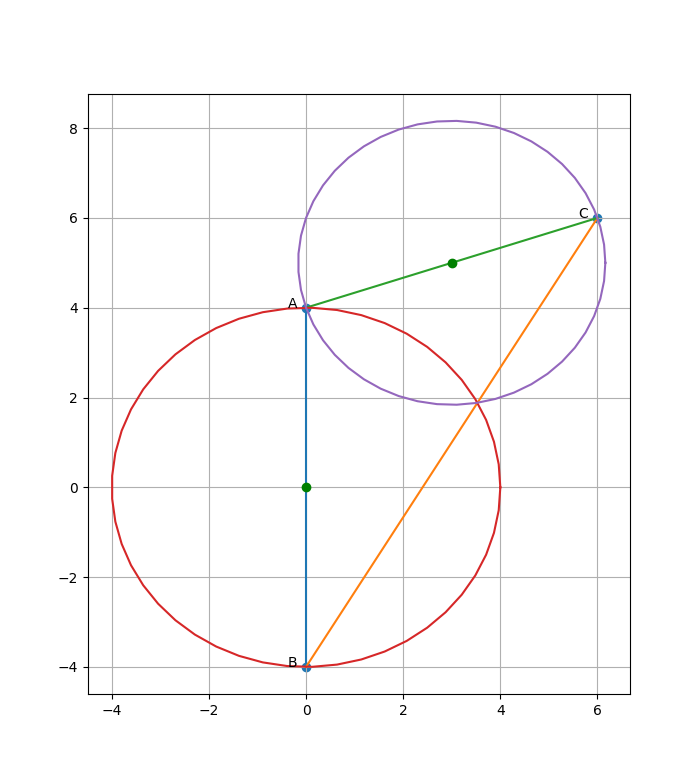
\includegraphics[width = \columnwidth]{chapters/9/10/5/10/figs/fig.png}
\caption{Graph}
\label{fig:chapters/9/10/5/10/1}
\end{figure}


    \item Prove that a cyclic paralellogram is a rectangle.
\label{chapters/9/10/5/12}
\\
\solution
\iffalse
\documentclass[journal,12pt,twocolumn]{IEEEtran}
\usepackage{setspace}
\usepackage{gensymb}
\usepackage{xcolor}
\usepackage{caption}
\singlespacing
\usepackage{siunitx}
\usepackage[cmex10]{amsmath}
\usepackage{mathtools}
\usepackage{hyperref}
\usepackage{amsthm}
\usepackage{mathrsfs}
\usepackage{txfonts}
\usepackage{stfloats}
\usepackage{cite}
\usepackage{cases}
\usepackage{subfig}
\usepackage{longtable}
\usepackage{multirow}
\usepackage{enumitem}
\usepackage{bm}
\usepackage{mathtools}
\usepackage{listings}
\usepackage{tikz}
\usetikzlibrary{shapes,arrows,positioning}
\usepackage{circuitikz}
\renewcommand{\vec}[1]{\boldsymbol{\mathbf{#1}}}
\DeclareMathOperator*{\Res}{Res}
\renewcommand\thesection{\arabic{section}}
\renewcommand\thesubsection{\thesection.\arabic{subsection}}
\renewcommand\thesubsubsection{\thesubsection.\arabic{subsubsection}}

\renewcommand\thesectiondis{\arabic{section}}
\renewcommand\thesubsectiondis{\thesectiondis.\arabic{subsection}}
\renewcommand\thesubsubsectiondis{\thesubsectiondis.\arabic{subsubsection}}
\hyphenation{op-tical net-works semi-conduc-tor}

\lstset{
language=Python,
frame=single, 
breaklines=true,
columns=fullflexible
}
\begin{document}
\theoremstyle{definition}
\newtheorem{theorem}{Theorem}[section]
\newtheorem{problem}{Problem}
\newtheorem{proposition}{Proposition}[section]
\newtheorem{lemma}{Lemma}[section]
\newtheorem{corollary}[theorem]{Corollary}
\newtheorem{example}{Example}[section]
\newtheorem{definition}{Definition}[section]
\newcommand{\BEQA}{\begin{eqnarray}}
\newcommand{\EEQA}{\end{eqnarray}}
\newcommand{\define}{\stackrel{\triangle}{=}}
\newcommand{\myvec}[1]{\ensuremath{\begin{pmatrix}#1\end{pmatrix}}}
\newcommand{\mydet}[1]{\ensuremath{\begin{vmatrix}#1\end{vmatrix}}}
\bibliographystyle{IEEEtran}
\providecommand{\nCr}[2]{\,^{#1}C_{#2}} % nCr
\providecommand{\nPr}[2]{\,^{#1}P_{#2}} % nPr
\providecommand{\mbf}{\mathbf}
\providecommand{\pr}[1]{\ensuremath{\Pr\left(#1\right)}}
\providecommand{\qfunc}[1]{\ensuremath{Q\left(#1\right)}}
\providecommand{\sbrak}[1]{\ensuremath{{}\left[#1\right]}}
\providecommand{\lsbrak}[1]{\ensuremath{{}\left[#1\right.}}
\providecommand{\rsbrak}[1]{\ensuremath{{}\left.#1\right]}}
\providecommand{\brak}[1]{\ensuremath{\left(#1\right)}}
\providecommand{\lbrak}[1]{\ensuremath{\left(#1\right.}}
\providecommand{\rbrak}[1]{\ensuremath{\left.#1\right)}}
\providecommand{\cbrak}[1]{\ensuremath{\left\{#1\right\}}}
\providecommand{\lcbrak}[1]{\ensuremath{\left\{#1\right.}}
\providecommand{\rcbrak}[1]{\ensuremath{\left.#1\right\}}}
\theoremstyle{remark}
\newtheorem{rem}{Remark}
\newcommand{\sgn}{\mathop{\mathrm{sgn}}}
\newcommand{\rect}{\mathop{\mathrm{rect}}}
\newcommand{\sinc}{\mathop{\mathrm{sinc}}}
\providecommand{\abs}[1]{\left\vert#1\right\vert}
\providecommand{\res}[1]{\Res\displaylimits_{#1}} 
\providecommand{\norm}[1]{\left\Vert#1\right\Vert}
\providecommand{\mtx}[1]{\mathbf{#1}}
\providecommand{\mean}[1]{E\left[ #1 \right]}
\providecommand{\fourier}{\overset{\mathcal{F}}{ \rightleftharpoons}}
\providecommand{\ztrans}{\overset{\mathcal{Z}}{ \rightleftharpoons}}
\providecommand{\system}[1]{\overset{\mathcal{#1}}{ \longleftrightarrow}}
\newcommand{\solution}{\noindent \textbf{Solution: }}
\providecommand{\dec}[2]{\ensuremath{\overset{#1}{\underset{#2}{\gtrless}}}}
\let\StandardTheFigure\thefigure
\def\putbox#1#2#3{\makebox[0in][l]{\makebox[#1][l]{}\raisebox{\baselineskip}[0in][0in]{\raisebox{#2}[0in][0in]{#3}}}}
     \def\rightbox#1{\makebox[0in][r]{#1}}
     \def\centbox#1{\makebox[0in]{#1}}
     \def\topbox#1{\raisebox{-\baselineskip}[0in][0in]{#1}}
     \def\midbox#1{\raisebox{-0.5\baselineskip}[0in][0in]{#1}}

\vspace{3cm}
\title{Circle Assignment}
\author{Gautam Singh}
\maketitle
\bigskip

\begin{abstract}
    This document contains the solution to Question 12 of 
    Exercise 5 in Chapter 10 of the class 9 NCERT textbook.
\end{abstract}

\begin{enumerate}

    \solution 
\fi
		Consider the points $\vec{P_i},\ 1 \le i \le 4$ in anticlockwise 
    order on the unit circle. Thus, for $1 \le i \le 4$,
    \begin{align}
        \vec{P_i} = \myvec{\cos\theta_i\\\sin\theta_i} 
        \label{eq:chapters/9/10/5/12/circ-point}
    \end{align}
    where 
    \begin{align}
        \theta_i \in [0,2\pi),\ i \neq j \iff \theta_i \neq \theta_j
        \label{eq:chapters/9/10/5/12/theta-cond}
    \end{align}
    Without loss of generality, suppose that $P_1P_2$ and $P_3P_4$ are parallel 
    to the $x$-axis. Since
    \begin{align}
        \vec{P_1}-\vec{P_2} &= \myvec{\cos\theta_1-\cos\theta_2\\\sin\theta_1-\sin\theta_2} \\
        \vec{P_3}-\vec{P_4} &= \myvec{\cos\theta_4-\cos\theta_4\\\sin\theta_3-\sin\theta_4}
    \end{align}
    we have
    \begin{align}
        \sin\theta_1&=\sin\theta_2 \\
        \implies \theta_1&=n\pi+\brak{-1}^n\theta_2
        \label{eq:chapters/9/10/5/12/x-par}
    \end{align}
    However, \eqref{eq:chapters/9/10/5/12/theta-cond} forces $n \in \cbrak{1,3}$, thus
    \begin{align}
        \theta_1+\theta_2 \in \cbrak{\pi,3\pi}
        \label{eq:chapters/9/10/5/12/theta-12}
    \end{align}
    Similarly,
    \begin{align}
        \theta_3+\theta_4 \in \cbrak{\pi,3\pi}
        \label{eq:chapters/9/10/5/12/theta-34}
    \end{align}
    Since $P_1P_2P_3P_4$ is a parallelogram, its diagonals bisect each other. 
    Thus, using \eqref{eq:chapters/9/10/5/12/theta-12} and \eqref{eq:chapters/9/10/5/12/theta-34},
    \begin{align}
        \frac{\vec{P_1}+\vec{P_3}}{2} &= \frac{\vec{P_2}+\vec{P_4}}{2} \\
        \implies \vec{P_1}+\vec{P_3} &= \vec{P_2}+\vec{P_4} \\
        \implies \myvec{\cos\theta_1+\cos\theta_3\\\sin\theta_1+\sin\theta_3} &= \myvec{\cos\theta_2+\cos\theta_4\\\sin\theta_2+\sin\theta_4} \\
        \implies \cos\theta_1+\cos\theta_3 &= \cos\theta_2+\cos\theta_4 \\
                                           &= -\brak{\cos\theta_1+\cos\theta_3} \\
        \implies \cos\theta_1+\cos\theta_3 &= \cos\theta_2+\cos\theta_4 = 0
        \label{eq:chapters/9/10/5/12/cos-diag}
    \end{align}
    Using \eqref{eq:chapters/9/10/5/12/cos-diag}, \eqref{eq:chapters/9/10/5/12/theta-12} and \eqref{eq:chapters/9/10/5/12/theta-34}, we have
    \begin{align}
        \cos\theta_1 &= -\cos\theta_3 = \cos\theta_4 \\
        \cos\theta_2 &= -\cos\theta_4 = \cos\theta_3
        \label{eq:chapters/9/10/5/12/theta-14-23}
    \end{align}
    Thus,
    \begin{align}
        \vec{P_1} - \vec{P_4} &= \myvec{\cos\theta_1-\cos\theta_4\\\sin\theta_1-\sin\theta_4} \\
                              &= \myvec{0\\\sin\theta_1-\sin\theta_4}
                              \label{eq:chapters/9/10/5/12/p1p4}
    \end{align}
    Thus, from \eqref{eq:chapters/9/10/5/12/p1p4},
    \begin{align}
        &\brak{\vec{P_1}-\vec{P_2}}^\top\brak{\vec{P_1}-\vec{P_4}} \nonumber \\
        &= \myvec{\cos\theta_1-\cos\theta_2&0}\myvec{0\\\sin\theta_1-\sin\theta_4} = 0
        \label{eq:chapters/9/10/5/12/adj-perp}
    \end{align}
    From \eqref{eq:chapters/9/10/5/12/adj-perp}, we see that $P_1P_2 \perp P_1P_4$. Hence, $P_1P_2P_3P_4$ is
    a rectangle.

    The situation is demonstrated in Fig. \ref{fig:chapters/9/10/5/12/circle}, plotted by the Python
    code \texttt{codes/circle.py}. The various input parameters are shown in Table
    \ref{tab:chapters/9/10/5/12/param}.
    \begin{table}[!ht]
        \centering
        \begin{tabular}{|c|c|}
            \hline
            \textbf{Parameter} & \textbf{Value} \\
            \hline
            $r$ & 1 \\
            \hline
            $\theta_1$ & $\frac{\pi}{6}$ \\
            \hline
            $\theta_2$ & $\frac{5\pi}{6}$ \\
            \hline
            $\theta_3$ & $\frac{7\pi}{6}$ \\
            \hline
            $\theta_4$ & $\frac{11\pi}{6}$ \\
            \hline
        \end{tabular}
        \caption{Parameters used in the construction of Fig. \ref{fig:chapters/9/10/5/12/circle}.}
        \label{tab:chapters/9/10/5/12/param}
    \end{table}
    
    \begin{figure}[!ht]
        \centering
        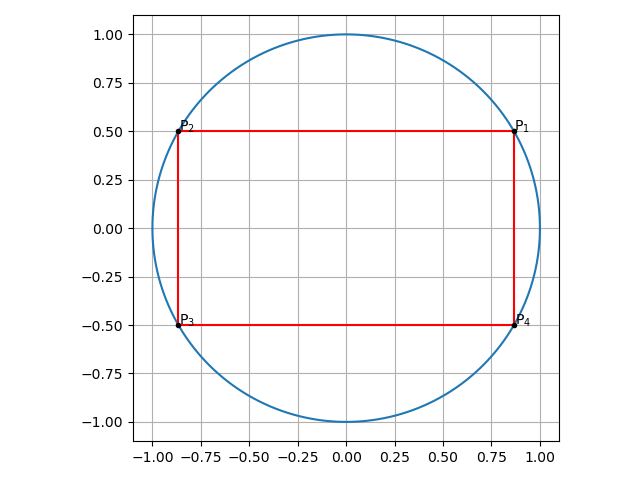
\includegraphics[width=\columnwidth]{chapters/9/10/5/12/figs/circle.png}
        \caption{$P_1P_2P_3P_4$ is a rectangle.}
        \label{fig:chapters/9/10/5/12/circle}
    \end{figure}

\item Prove that the line of centres of two intersecting circles subtends equal angles at the two points of intersection.
\\
    \solution 
\label{chapters/9/10/6/1}
\iffalse
\documentclass[12pt]{article}
\usepackage{graphicx}
\usepackage{amsmath}
\usepackage{mathtools}
\usepackage{gensymb}
\usepackage{amssymb}
\usepackage{tikz}
\usetikzlibrary{arrows,shapes,automata,petri,positioning,calc}
\usepackage{hyperref}
\usepackage{tikz}
\usetikzlibrary{matrix,calc}
\usepackage[margin=0.5in]{geometry}

\providecommand{\norm}[1]{\left\lVert#1\right\rVert}
\newcommand{\myvec}[1]{\ensuremath{\begin{pmatrix}#1\end{pmatrix}}}
\let\vec\mathbf
%\providecommand $${\norm}[1]{\left\lVert#1\right\rVert}$$
\providecommand{\abs}[1]{\left\vert#1\right\vert}
\let\vec\mathbf

\newcommand{\mydet}[1]{\ensuremath{\begin{vmatrix}#1\end{vmatrix}}}
\providecommand{\brak}[1]{\ensuremath{\left(#1\right)}}
\providecommand{\lbrak}[1]{\ensuremath{\left(#1\right.}}
\providecommand{\rbrak}[1]{\ensuremath{\left.#1\right)}}
\providecommand{\sbrak}[1]{\ensuremath{{}\left[#1\right]}}

\providecommand{\brak}[1]{\ensuremath{\left(#1\right)}}
\providecommand{\norm}[1]{\left\lVert#1\right\rVert}
\newcommand{\solution}{\noindent \textbf{Solution: }}

\let\vec\mathbf
\def\inputGnumericTable{}
\usepackage{color}                                            %%
    \usepackage{array}                                            %%
    \usepackage{longtable}                                        %%
    \usepackage{calc}                                             %%
    \usepackage{multirow}                                         %%
    \usepackage{hhline}                                           %%
    \usepackage{ifthen}
\usepackage{array}
\usepackage{amsmath}   % for having text in math mode
\usepackage{listings}
\lstset{
language=tex,
frame=single, 
breaklines=true
}
\newenvironment{Figure}
  {\par\medskip\noindent\minipage{\linewidth}}
  {\endminipage\par\medskip}
\begin{document}
\begin{center}
\textbf\large{CLASS-9\\CHAPTER-10 \\ CIRCLES}

\end{center}
\section*{Excercise 10.6}

\section*{\large Solution}:
\fi
The input parameters are available in Table 
	\ref{tab:chapters/9/10/6/1/table1}.
\begin{figure}[h!]
\centering
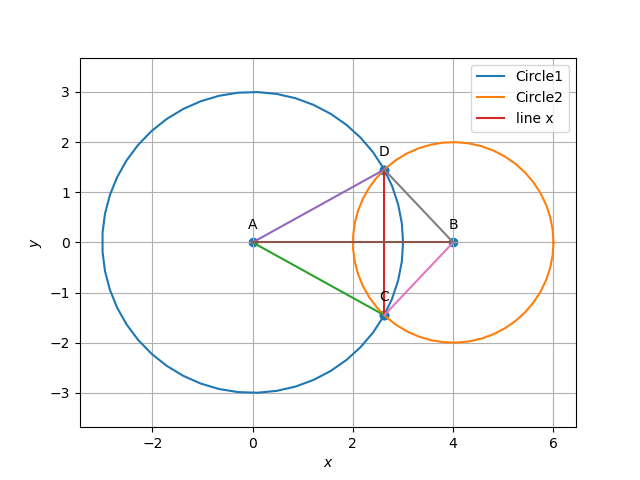
\includegraphics[width=\columnwidth]{chapters/9/10/6/1/figs/circle3.png}
\caption{}
\label{fig:chapters/9/10/6/1/Fig1}
\end{figure}



\begin{table}[h!]
	\small
	\centering
	%\subimport{../chapters/9/10/6/1/tables/}{table1.tex}
     %%%%%%%%%%%%%%%%%%%%%%%%%%%%%%%%%%%%%%%%%%%%%%%%%%%%%%%%%%%%%%%%%%%%%%
%%                                                                  %%
%%  This is the header of a LaTeX2e file exported from Gnumeric.    %%
%%                                                                  %%
%%  This file can be compiled as it stands or included in another   %%
%%  LaTeX document. The table is based on the longtable package so  %%
%%  the longtable options (headers, footers...) can be set in the   %%
%%  preamble section below (see PRAMBLE).                           %%
%%                                                                  %%
%%  To include the file in another, the following two lines must be %%
%%  in the including file:                                          %%
%%        \def\inputGnumericTable{}                                 %%
%%  at the beginning of the file and:                               %%
%%        \input{name-of-this-file.tex}                             %%
%%  where the table is to be placed. Note also that the including   %%
%%  file must use the following packages for the table to be        %%
%%  rendered correctly:                                             %%
%%    \usepackage[latin1]{inputenc}                                 %%
%%    \usepackage{color}                                            %%
%%    \usepackage{array}                                            %%
%%    \usepackage{longtable}                                        %%
%%    \usepackage{calc}                                             %%
%%    \usepackage{multirow}                                         %%
%%    \usepackage{hhline}                                           %%
%%    \usepackage{ifthen}                                           %%
%%  optionally (for landscape tables embedded in another document): %%
%%    \usepackage{lscape}                                           %%
%%                                                                  %%
%%%%%%%%%%%%%%%%%%%%%%%%%%%%%%%%%%%%%%%%%%%%%%%%%%%%%%%%%%%%%%%%%%%%%



%%  This section checks if we are begin input into another file or  %%
%%  the file will be compiled alone. First use a macro taken from   %%
%%  the TeXbook ex 7.7 (suggestion of Han-Wen Nienhuys).            %%
\def\ifundefined#1{\expandafter\ifx\csname#1\endcsname\relax}


%%  Check for the \def token for inputed files. If it is not        %%
%%  defined, the file will be processed as a standalone and the     %%
%%  preamble will be used.                                          %%
\ifundefined{inputGnumericTable}

%%  We must be able to close or not the document at the end.        %%
	\def\gnumericTableEnd{\end{document}}


%%%%%%%%%%%%%%%%%%%%%%%%%%%%%%%%%%%%%%%%%%%%%%%%%%%%%%%%%%%%%%%%%%%%%%
%%                                                                  %%
%%  This is the PREAMBLE. Change these values to get the right      %%
%%  paper size and other niceties.                                  %%
%%                                                                  %%
%%%%%%%%%%%%%%%%%%%%%%%%%%%%%%%%%%%%%%%%%%%%%%%%%%%%%%%%%%%%%%%%%%%%%%

	\documentclass[12pt%
			  %,landscape%
                    ]{report}
       \usepackage[latin1]{inputenc}
       \usepackage{fullpage}
       \usepackage{color}
       \usepackage{array}
       \usepackage{longtable}
       \usepackage{calc}
       \usepackage{multirow}
       \usepackage{hhline}
       \usepackage{ifthen}
       \usepackage{gensymb}
       \usepackage{graphicx}
\usepackage{amsmath}
\usepackage{mathtools}
\newcommand{\mydet}[1]{\ensuremath{\begin{vmatrix}#1\end{vmatrix}}}
\providecommand{\brak}[1]{\ensuremath{\left(#1\right)}}
\providecommand{\norm}[1]{\left\lVert#1\right\rVert}
\newcommand{\solution}{\noindent \textbf{Solution: }}
\newcommand{\myvec}[1]{\ensuremath{\begin{pmatrix}#1\end{pmatrix}}}
\let\vec\mathbf
	\begin{document}


%%  End of the preamble for the standalone. The next section is for %%
%%  documents which are included into other LaTeX2e files.          %%
\else

%%  We are not a stand alone document. For a regular able, we will %%
%%  have no preamble and only define the closing to mean nothing.   %%
    \def\gnumericTableEnd{}

%%  If we want landscape mode in an embedded document, comment out  %%
%%  the line above and uncomment the two below. The table will      %%
%%  begin on a new page and run in landscape mode.                  %%
%       \def\gnumericTableEnd{\end{landscape}}
%       \begin{landscape}


%%  End of the else clause for this file being \input.              %%
\fi

%%%%%%%%%%%%%%%%%%%%%%%%%%%%%%%%%%%%%%%%%%%%%%%%%%%%%%%%%%%%%%%%%%%%%%
%%                                                                  %%
%%  The rest is the gnumeric table, except for the closing          %%
%%  statement. Changes below will alter the table's appearance.     %%
%%                                                                  %%
%%%%%%%%%%%%%%%%%%%%%%%%%%%%%%%%%%%%%%%%%%%%%%%%%%%%%%%%%%%%%%%%%%%%%%
\providecommand{\gnumericmathit}[1]{#1} 
%%  Uncomment the next line if you would like your numbers to be in %%
%%  italics if they are italizised in the gnumeric table.           %%
%\renewcommand{\gnumericmathit}[1]{\mathit{#1}}
\providecommand{\gnumericPB}[1]%
{\let\gnumericTemp=\\#1\let\\=\gnumericTemp\hspace{0pt}}
 \ifundefined{gnumericTableWidthDefined}
        \newlength{\gnumericTableWidth}
        \newlength{\gnumericTableWidthComplete}
        \newlength{\gnumericMultiRowLength}
        \global\def\gnumericTableWidthDefined{}
 \fi
%% The following setting protects this code from babel shorthands.  %%
 \ifthenelse{\isundefined{\languageshorthands}}{}{\languageshorthands{english}}
%%  The default table format retains the relative column widths of  %%
%%  gnumeric. They can easily be changed to c, r or l. In that case %%
%%  you may want to comment out the next line and uncomment the one %%
%%  thereafter                                                      %%
\providecommand\gnumbox{\makebox[0pt]}
%%\providecommand\gnumbox[1][]{\makebox}

%% to adjust positions in multirow situations                       %%
\setlength{\bigstrutjot}{\jot}
\setlength{\extrarowheight}{\doublerulesep}

%%  The \setlongtables command keeps column widths the same across  %%
%%  pages. Simply comment out next line for varying column widths.  %%
\setlongtables

\setlength\gnumericTableWidth{%
	40pt+%
	35pt+%
	210pt+%
0pt}
\def\gumericNumCols{3}
\setlength\gnumericTableWidthComplete{\gnumericTableWidth+%
         \tabcolsep*\gumericNumCols*2+\arrayrulewidth*\gumericNumCols}
\ifthenelse{\lengthtest{\gnumericTableWidthComplete > \linewidth}}%
         {\def\gnumericScale{\ratio{\linewidth-%
                        \tabcolsep*\gumericNumCols*2-%
                        \arrayrulewidth*\gumericNumCols}%
{\gnumericTableWidth}}}%
{\def\gnumericScale{1}}

%%%%%%%%%%%%%%%%%%%%%%%%%%%%%%%%%%%%%%%%%%%%%%%%%%%%%%%%%%%%%%%%%%%%%%
%%                                                                  %%
%% The following are the widths of the various columns. We are      %%
%% defining them here because then they are easier to change.       %%
%% Depending on the cell formats we may use them more than once.    %%
%%                                                                  %%
%%%%%%%%%%%%%%%%%%%%%%%%%%%%%%%%%%%%%%%%%%%%%%%%%%%%%%%%%%%%%%%%%%%%%%

\ifthenelse{\isundefined{\gnumericColA}}{\newlength{\gnumericColA}}{}\settowidth{\gnumericColA}{\begin{tabular}{@{}p{40pt*\gnumericScale}@{}}x\end{tabular}}
\ifthenelse{\isundefined{\gnumericColB}}{\newlength{\gnumericColB}}{}\settowidth{\gnumericColB}{\begin{tabular}{@{}p{35pt*\gnumericScale}@{}}x\end{tabular}}
\ifthenelse{\isundefined{\gnumericColC}}{\newlength{\gnumericColC}}{}\settowidth{\gnumericColC}{\begin{tabular}{@{}p{210pt*\gnumericScale}@{}}x\end{tabular}}

\begin{longtable}[c]{%
	b{\gnumericColA}%
	b{\gnumericColB}%
	b{\gnumericColC}%
	}

%%%%%%%%%%%%%%%%%%%%%%%%%%%%%%%%%%%%%%%%%%%%%%%%%%%%%%%%%%%%%%%%%%%%%%
%%  The longtable options. (Caption, headers... see Goosens, p.124) %%
%	\caption{The Table Caption.}             \\	%
% \hline	% Across the top of the table.
%%  The rest of these options are table rows which are placed on    %%
%%  the first, last or every page. Use \multicolumn if you want.    %%

%%  Header for the first page.                                      %%
%	\multicolumn{3}{c}{The First Header} \\ \hline 
%	\multicolumn{1}{c}{colTag}	%Column 1
%	&\multicolumn{1}{c}{colTag}	%Column 2
%	&\multicolumn{1}{c}{colTag}	\\ \hline %Last column
%	\endfirsthead

%%  The running header definition.                                  %%
%	\hline
%	\multicolumn{3}{l}{\ldots\small\slshape continued} \\ \hline
%	\multicolumn{1}{c}{colTag}	%Column 1
%	&\multicolumn{1}{c}{colTag}	%Column 2
%	&\multicolumn{1}{c}{colTag}	\\ \hline %Last column
%	\endhead

%%  The running footer definition.                                  %%
%	\hline
%	\multicolumn{3}{r}{\small\slshape continued\ldots} \\
%	\endfoot

%%  The ending footer definition.                                   %%
%	\multicolumn{3}{c}{That's all folks} \\ \hline 
%	\endlastfoot
%%%%%%%%%%%%%%%%%%%%%%%%%%%%%%%%%%%%%%%%%%%%%%%%%%%%%%%%%%%%%%%%%%%%%%

\hhline{|-|-|-}
	 \multicolumn{1}{|p{\gnumericColA}|}%
	{\gnumericPB{\raggedright}\gnumbox[l]{\textbf{Symbol}}}
	&\multicolumn{1}{p{\gnumericColB}|}%
	{\gnumericPB{\raggedright}\gnumbox[l]{\textbf{Values}}}
	&\multicolumn{1}{p{\gnumericColC}|}%
	{\gnumericPB{\raggedright}\gnumbox[l]{\textbf{Description}}}
\\
\hhline{|---|}
	 \multicolumn{1}{|p{\gnumericColA}|}%
	{\gnumericPB{\raggedright}\gnumbox[l]{$\vec{A}$}}
	&\multicolumn{1}{p{\gnumericColB}|}%
	{\gnumericPB{\raggedright}\gnumbox[l]{\myvec{0\\0}}}
	&\multicolumn{1}{p{\gnumericColC}|}%
	{\gnumericPB{\raggedright}\gnumbox[l]{Center of circle 1}}
\\
\hhline{|---|}
	 \multicolumn{1}{|p{\gnumericColA}|}%
	{\gnumericPB{\raggedright}\gnumbox[l]{$r_1$}}
	&\multicolumn{1}{p{\gnumericColB}|}%
	{\gnumericPB{\raggedright}\gnumbox[l]{3 units}}
	&\multicolumn{1}{p{\gnumericColC}|}%
	{\gnumericPB{\raggedright}\gnumbox[l]{Radius of the circle 1 }}
\\
\hhline{|---|}
	 \multicolumn{1}{|p{\gnumericColA}|}%
	{\gnumericPB{\raggedright}\gnumbox[l]{$\vec{B}$}}
	&\multicolumn{1}{p{\gnumericColB}|}%
	{\gnumericPB{\raggedright}\gnumbox[l]{\myvec{4\\0}}}
	&\multicolumn{1}{p{\gnumericColC}|}%
	{\gnumericPB{\raggedright}\gnumbox[l]{Center of circle 2}}
\\
\hhline{|---|}
	 \multicolumn{1}{|p{\gnumericColA}|}%
	{\gnumericPB{\raggedright}\gnumbox[l]{$r_2$}}
	&\multicolumn{1}{p{\gnumericColB}|}%
	{\gnumericPB{\raggedright}\gnumbox[l]{2 units}}
	&\multicolumn{1}{p{\gnumericColC}|}%
	{\gnumericPB{\raggedright}\gnumbox[l]{Radius of circle 2}}
\\
\hhline{|---|}
	 \multicolumn{1}{|p{\gnumericColA}|}%
	{\gnumericPB{\raggedright}\gnumbox[l]{$\vec{e}_1$}}
	&\multicolumn{1}{p{\gnumericColB}|}%
	{\gnumericPB{\raggedright}\gnumbox[l]{\myvec{1\\0}}}
	&\multicolumn{1}{p{\gnumericColC}|}%
	{\gnumericPB{\raggedright}\gnumbox[l]{Standard basis vector 1}}
\\
\hhline{|---|}
\multicolumn{1}{|p{\gnumericColA}|}%
	{\gnumericPB{\raggedright}\gnumbox[l]{$\vec{e}_2$}}
	&\multicolumn{1}{p{\gnumericColB}|}%
	{\gnumericPB{\raggedright}\gnumbox[l]{\myvec{0\\1}}}
	&\multicolumn{1}{p{\gnumericColC}|}%
	{\gnumericPB{\raggedright}\gnumbox[l]{Standard basis vector 2}}
	\\
\hhline{|---|}
\end{longtable}

\ifthenelse{\isundefined{\languageshorthands}}{}{\languageshorthands{\languagename}}
\gnumericTableEnd%t
%	\caption{}
	\label{tab:chapters/9/10/6/1/table1}
\end{table}
 The two circle equations are given by
\begin{align}
\label{eq:chapters/9/10/6/1/1}
	\norm{x}^2-9&=0\\
	\norm{x}^2-8\vec{e}_1+12&=0
\end{align}
yielding the intersection of the circles as the line
\begin{align}
\myvec{1&0}\vec{x}&=\frac{21}{8}\\
\label{eq:chapters/9/10/6/1/20}
\end{align}
		\eqref{eq:chapters/9/10/6/1/20} can be expressed as
\begin{align}
	\vec{x}=\vec{q}+\lambda\vec{m}\label{eq:chapters/9/10/6/1/21}
\end{align}
The distance form origin to point $\vec{x}$ is given by
\begin{align}
	\norm{\vec{x}}^2&=d^2\label{eq:chapters/9/10/6/1/22}
\end{align}
		Then substituting \eqref{eq:chapters/9/10/6/1/21} in \eqref{eq:chapters/9/10/6/1/22} yeilds,
\begin{align}
	\brak{\vec{q}+\lambda\vec{m}}^{\top}\brak{\vec{q}+\lambda\vec{m}}&=d^2\\
	\implies \lambda^2\norm{\vec{m}}^2+2\lambda\vec{q}^{\top}\vec{m}+\norm{\vec{q}}^2&=d^2\label{eq:chapters/9/10/6/1/26}
\end{align}
where
\begin{align}
	\vec{q}=\myvec{\frac{21}{8}\\0},\vec{m}=\myvec{0\\1} \text{ and } d=r_1=3
	\label{eq:chapters/9/10/6/1/27}
\end{align}
		Substituting the values in \eqref{eq:chapters/9/10/6/1/27} in \eqref{eq:chapters/9/10/6/1/26}, 
\begin{align}
	\lambda^2(1)+2\lambda\myvec{\frac{21}{8}&0}\myvec{0\\1}+\frac{441}{64}&=9\\
	\implies\lambda_i&=\pm\frac{3\sqrt{5}}{8}
\end{align}
Thus, 
the intersecting points $\vec{C}$ and $\vec{D}$ are given by
\begin{align}
    \vec{C}&=\vec{q}+\lambda_1\vec{m}=\myvec{\frac{21}{8}\\[2pt]-\frac{3\sqrt{5}}{8}}\\
    \vec{D}&=\vec{q}+\lambda_2\vec{m}=\myvec{\frac{21}{8}\\[2pt]\frac{3\sqrt{5}}{8}}
\end{align}
\begin{enumerate}
\item Finding $\angle$ADB
	\begin{align}
		 \vec{A-D} = \myvec{-\frac{21}{8}\\[2pt]-\frac{3\sqrt{5}}{8}},
		\vec{B-D}& = \myvec{\frac{11}{8}\\[2pt]-\frac{3\sqrt{5}}{8}}\\
	 \vec{(A-D)^\top(B-D)}&= -\frac{3}{2}\\
	 \norm{\vec{A-D}}\norm{\vec{C-D}}& = 6\\
\implies		\cos(\angle ADB)& = \frac{\vec{(A-D)^\top(B-D)}}{\norm{\vec{A-D}}\norm{\vec{B-D}}}\\
		\text{or, }		\angle ADB&=104\degree
\end{align}
\item Finding $\angle$ACB
\begin{align}
	\vec{A-C} = \myvec{-\frac{21}{8}\\[2pt]\frac{3\sqrt{5}}{8}},
	 \vec{B-C}& = \myvec{\frac{11}{8}\\[2pt]\frac{3\sqrt{5}}{8}}\\
	 \vec{(A-C)^\top(B-C)}&= -\frac{3}{2}\\
	 \norm{\vec{A-C}}\norm{\vec{B-C}}& = 6\\
\implies 	 \cos(\angle ACB) &= \frac{\vec{(A-C)^\top(B-C)}}{\norm{\vec{A-C}}\norm{\vec{B-C}}}\\
	\text{or, }	 \angle ACB&=104\degree = \angle ADB
\end{align}
\end{enumerate}
See Fig. 
\ref{fig:chapters/9/10/6/1/Fig1}.



\item  $AC$ and $BD$ are chords of a circle which bisect each other. Prove that 
	\begin{enumerate}
		\item  $AC$ and $BD$ are diameters, 
		\item  $ABCD$ is a rectangle.
	\end{enumerate}
    \solution 
\label{chapters/9/10/6/7}
\iffalse
\documentclass[journal,12pt,twocolumn]{IEEEtran}
\def\inputGnumericTable{}
\usepackage{setspace}
\usepackage{gensymb}
\usepackage{xcolor}
\usepackage{caption}
\singlespacing
\usepackage{siunitx}
\usepackage[cmex10]{amsmath}
\usepackage{mathtools}
\usepackage{hyperref}
\usepackage{amsthm}
\usepackage{mathrsfs}
\usepackage{txfonts}
\usepackage{stfloats}
\usepackage{cite}
\usepackage{cases}
\usepackage{subfig}
\usepackage{longtable}
\usepackage{multirow}
\usepackage{enumitem}
\usepackage{mathtools}
\usepackage{listings}
\usepackage{tikz}
\usetikzlibrary{shapes,arrows,positioning}
\usepackage{circuitikz}
       \usepackage[latin1]{inputenc}
       \usepackage{fullpage}
       \usepackage{color}
       \usepackage{array}
       \usepackage{longtable}
       \usepackage{calc}
       \usepackage{multirow}
       \usepackage{hhline}
       \usepackage{ifthen}
	   \usepackage{setspace}
\let\vec\mathbf
\DeclareMathOperator*{\Res}{Res}
\renewcommand\thesection{\arabic{section}}
\renewcommand\thesubsection{\thesection.\arabic{subsection}}
\renewcommand\thesubsubsection{\thesubsection.\arabic{subsubsection}}

\renewcommand\thesectiondis{\arabic{section}}
\renewcommand\thesubsectiondis{\thesectiondis.\arabic{subsection}}
\renewcommand\thesubsubsectiondis{\thesubsectiondis.\arabic{subsubsection}}
\hyphenation{op-tical net-works semi-conduc-tor}

\lstset{
language=Python,
frame=single, 
breaklines=true,
columns=fullflexible
}
\begin{document}
\theoremstyle{definition}
\newtheorem{theorem}{Theorem}[section]
\newtheorem{problem}{Problem}
\newtheorem{proposition}{Proposition}[section]
\newtheorem{lemma}{Lemma}[section]
\newtheorem{corollary}[theorem]{Corollary}
\newtheorem{example}{Example}[section]
\newtheorem{definition}{Definition}[section]
\newcommand{\BEQA}{\begin{eqnarray}}
        \newcommand{\EEQA}{\end{eqnarray}}
\newcommand{\define}{\stackrel{\triangle}{=}}
\newcommand{\myvec}[1]{\ensuremath{\begin{pmatrix}#1\end{pmatrix}}}
\newcommand{\mydet}[1]{\ensuremath{\begin{vmatrix}#1\end{vmatrix}}}

\bibliographystyle{IEEEtran}
\providecommand{\nCr}[2]{\,^{#1}C_{#2}} % nCr
\providecommand{\nPr}[2]{\,^{#1}P_{#2}} % nPr
\providecommand{\mbf}{\mathbf}
\providecommand{\pr}[1]{\ensuremath{\Pr\left(#1\right)}}
\providecommand{\qfunc}[1]{\ensuremath{Q\left(#1\right)}}
\providecommand{\sbrak}[1]{\ensuremath{{}\left[#1\right]}}
\providecommand{\lsbrak}[1]{\ensuremath{{}\left[#1\right.}}
\providecommand{\rsbrak}[1]{\ensuremath{{}\left.#1\right]}}
\providecommand{\brak}[1]{\ensuremath{\left(#1\right)}}
\providecommand{\lbrak}[1]{\ensuremath{\left(#1\right.}}
\providecommand{\rbrak}[1]{\ensuremath{\left.#1\right)}}
\providecommand{\cbrak}[1]{\ensuremath{\left\{#1\right\}}}
\providecommand{\lcbrak}[1]{\ensuremath{\left\{#1\right.}}
\providecommand{\rcbrak}[1]{\ensuremath{\left.#1\right\}}}
\theoremstyle{remark}
\newtheorem{rem}{Remark}
\newcommand{\sgn}{\mathop{\mathrm{sgn}}}
\newcommand{\rect}{\mathop{\mathrm{rect}}}
\newcommand{\sinc}{\mathop{\mathrm{sinc}}}
\providecommand{\abs}[1]{\left\vert#1\right\vert}
\providecommand{\res}[1]{\Res\displaylimits_{#1}}
\providecommand{\norm}[1]{\lVert#1\rVert}
\providecommand{\mtx}[1]{\mathbf{#1}}
\providecommand{\mean}[1]{E\left[ #1 \right]}
\providecommand{\fourier}{\overset{\mathcal{F}}{ \rightleftharpoons}}
\providecommand{\ztrans}{\overset{\mathcal{Z}}{ \rightleftharpoons}}
\providecommand{\system}[1]{\overset{\mathcal{#1}}{ \longleftrightarrow}}
\newcommand{\solution}{\noindent \textbf{Solution: }}
\providecommand{\dec}[2]{\ensuremath{\overset{#1}{\underset{#2}{\gtrless}}}}
\let\StandardTheFigure\thefigure
\def\putbox#1#2#3{\makebox[0in][l]{\makebox[#1][l]{}\raisebox{\baselineskip}[0in][0in]{\raisebox{#2}[0in][0in]{#3}}}}
\def\rightbox#1{\makebox[0in][r]{#1}}
\def\centbox#1{\makebox[0in]{#1}}
\def\topbox#1{\raisebox{-\baselineskip}[0in][0in]{#1}}
\def\midbox#1{\raisebox{-0.5\baselineskip}[0in][0in]{#1}}

\vspace{3cm}
\title{\LaTeX\ 9.10.6.7}
\author{Lokesh Surana}
\maketitle
\section*{Class 9, Chapter, 10, Exercse 6.7}


\solution
\fi
Consider a unit circle with center at origin.
Let $AC$ and $BD$ be the diameters of the circle.
The points on circle that we consider are available in Table \eqref{tab:chapters/9/10/6/7/points}.
%
\begin{table}[ht!]
%%%%%%%%%%%%%%%%%%%%%%%%%%%%%%%%%%%%%%%%%%%%%%%%%%%%%%%%%%%%%%%%%%%%%%
%%                                                                  %%
%%  This is the header of a LaTeX2e file exported from Gnumeric.    %%
%%                                                                  %%
%%  This file can be compiled as it stands or included in another   %%
%%  LaTeX document. The table is based on the longtable package so  %%
%%  the longtable options (headers, footers...) can be set in the   %%
%%  preamble section below (see PRAMBLE).                           %%
%%                                                                  %%
%%  To include the file in another, the following two lines must be %%
%%  in the including file:                                          %%
%%        \def\inputGnumericTable{}                                 %%
%%  at the beginning of the file and:                               %%
%%        \input{name-of-this-file.tex}                             %%
%%  where the table is to be placed. Note also that the including   %%
%%  file must use the following packages for the table to be        %%
%%  rendered correctly:                                             %%
%%    \usepackage[latin1]{inputenc}                                 %%
%%    \usepackage{color}                                            %%
%%    \usepackage{array}                                            %%
%%    \usepackage{longtable}                                        %%
%%    \usepackage{calc}                                             %%
%%    \usepackage{multirow}                                         %%
%%    \usepackage{hhline}                                           %%
%%    \usepackage{ifthen}                                           %%
%%  optionally (for landscape tables embedded in another document): %%
%%    \usepackage{lscape}                                           %%
%%                                                                  %%
%%%%%%%%%%%%%%%%%%%%%%%%%%%%%%%%%%%%%%%%%%%%%%%%%%%%%%%%%%%%%%%%%%%%%%



%%  This section checks if we are begin input into another file or  %%
%%  the file will be compiled alone. First use a macro taken from   %%
%%  the TeXbook ex 7.7 (suggestion of Han-Wen Nienhuys).            %%
\def\ifundefined#1{\expandafter\ifx\csname#1\endcsname\relax}


%%  Check for the \def token for inputed files. If it is not        %%
%%  defined, the file will be processed as a standalone and the     %%
%%  preamble will be used.                                          %%
\ifundefined{inputGnumericTable}

%%  We must be able to close or not the document at the end.        %%
	\def\gnumericTableEnd{\end{document}}


%%%%%%%%%%%%%%%%%%%%%%%%%%%%%%%%%%%%%%%%%%%%%%%%%%%%%%%%%%%%%%%%%%%%%%
%%                                                                  %%
%%  This is the PREAMBLE. Change these values to get the right      %%
%%  paper size and other niceties.                                  %%
%%                                                                  %%
%%%%%%%%%%%%%%%%%%%%%%%%%%%%%%%%%%%%%%%%%%%%%%%%%%%%%%%%%%%%%%%%%%%%%%

	\documentclass[12pt%
			  %,landscape%
                    ]{report}
       \usepackage[latin1]{inputenc}
       \usepackage{fullpage}
       \usepackage{color}
       \usepackage{array}
       \usepackage{longtable}
       \usepackage{calc}
       \usepackage{multirow}
       \usepackage{hhline}
       \usepackage{ifthen}
	   \usepackage{setspace}

%%  End of the preamble for the standalone. The next section is for %%
%%  documents which are included into other LaTeX2e files.          %%
\else

%%  We are not a stand alone document. For a regular table, we will %%
%%  have no preamble and only define the closing to mean nothing.   %%
    \def\gnumericTableEnd{}

%%  If we want landscape mode in an embedded document, comment out  %%
%%  the line above and uncomment the two below. The table will      %%
%%  begin on a new page and run in landscape mode.                  %%
%       \def\gnumericTableEnd{\end{landscape}}
%       \begin{landscape}


%%  End of the else clause for this file being \input.              %%
\fi

%%%%%%%%%%%%%%%%%%%%%%%%%%%%%%%%%%%%%%%%%%%%%%%%%%%%%%%%%%%%%%%%%%%%%%
%%                                                                  %%
%%  The rest is the gnumeric table, except for the closing          %%
%%  statement. Changes below will alter the table's appearance.     %%
%%                                                                  %%
%%%%%%%%%%%%%%%%%%%%%%%%%%%%%%%%%%%%%%%%%%%%%%%%%%%%%%%%%%%%%%%%%%%%%%

\providecommand{\gnumericmathit}[1]{#1} 
%%  Uncomment the next line if you would like your numbers to be in %%
%%  italics if they are italizised in the gnumeric table.           %%
%\renewcommand{\gnumericmathit}[1]{\mathit{#1}}
\providecommand{\gnumericPB}[1]%
{\let\gnumericTemp=\\#1\let\\=\gnumericTemp\hspace{0pt}}
 \ifundefined{gnumericTableWidthDefined}
        \newlength{\gnumericTableWidth}
        \newlength{\gnumericTableWidthComplete}
        \newlength{\gnumericMultiRowLength}
        \global\def\gnumericTableWidthDefined{}
 \fi
%% The following setting protects this code from babel shorthands.  %%
 \ifthenelse{\isundefined{\languageshorthands}}{}{\languageshorthands{english}}
%%  The default table format retains the relative column widths of  %%
%%  gnumeric. They can easily be changed to c, r or l. In that case %%
%%  you may want to comment out the next line and uncomment the one %%
%%  thereafter                                                      %%
\providecommand\gnumbox{\makebox[0pt]}
%%\providecommand\gnumbox[1][]{\makebox}

%% to adjust positions in multirow situations                       %%
\setlength{\bigstrutjot}{\jot}
\setlength{\extrarowheight}{\doublerulesep}

%%  The \setlongtables command keeps column widths the same across  %%
%%  pages. Simply comment out next line for varying column widths.  %%
\setlongtables

\setlength\gnumericTableWidth{%
	53pt+%
	90pt+%
	54pt+%
0pt}
\def\gumericNumCols{3}
\setlength\gnumericTableWidthComplete{\gnumericTableWidth+%
         \tabcolsep*\gumericNumCols*2+\arrayrulewidth*\gumericNumCols}
\ifthenelse{\lengthtest{\gnumericTableWidthComplete > \linewidth}}%
         {\def\gnumericScale{1*\ratio{\linewidth-%
                        \tabcolsep*\gumericNumCols*2-%
                        \arrayrulewidth*\gumericNumCols}%
{\gnumericTableWidth}}}%
{\def\gnumericScale{1}}

%%%%%%%%%%%%%%%%%%%%%%%%%%%%%%%%%%%%%%%%%%%%%%%%%%%%%%%%%%%%%%%%%%%%%%
%%                                                                  %%
%% The following are the widths of the various columns. We are      %%
%% defining them here because then they are easier to change.       %%
%% Depending on the cell formats we may use them more than once.    %%
%%                                                                  %%
%%%%%%%%%%%%%%%%%%%%%%%%%%%%%%%%%%%%%%%%%%%%%%%%%%%%%%%%%%%%%%%%%%%%%%

\ifthenelse{\isundefined{\gnumericColA}}{\newlength{\gnumericColA}}{}\settowidth{\gnumericColA}{\begin{tabular}{@{}p{53pt*\gnumericScale}@{}}x\end{tabular}}
\ifthenelse{\isundefined{\gnumericColB}}{\newlength{\gnumericColB}}{}\settowidth{\gnumericColB}{\begin{tabular}{@{}p{90pt*\gnumericScale}@{}}x\end{tabular}}
\ifthenelse{\isundefined{\gnumericColC}}{\newlength{\gnumericColC}}{}\settowidth{\gnumericColC}{\begin{tabular}{@{}p{54pt*\gnumericScale}@{}}x\end{tabular}}

\begin{tabular}[c]{%
	b{\gnumericColA}%
	b{\gnumericColB}%
	b{\gnumericColC}%
	}

%%%%%%%%%%%%%%%%%%%%%%%%%%%%%%%%%%%%%%%%%%%%%%%%%%%%%%%%%%%%%%%%%%%%%%
%%  The longtable options. (Caption, headers... see Goosens, p.124) %%
%	\caption{The Table Caption.}             \\	%
% \hline	% Across the top of the table.
%%  The rest of these options are table rows which are placed on    %%
%%  the first, last or every page. Use \multicolumn if you want.    %%

%%  Header for the first page.                                      %%
%	\multicolumn{3}{c}{The First Header} \\ \hline 
%	\multicolumn{1}{c}{colTag}	%Column 1
%	&\multicolumn{1}{c}{colTag}	%Column 2
%	&\multicolumn{1}{c}{colTag}	\\ \hline %Last column
%	\endfirsthead

%%  The running header definition.                                  %%
%	\hline
%	\multicolumn{3}{l}{\ldots\small\slshape continued} \\ \hline
%	\multicolumn{1}{c}{colTag}	%Column 1
%	&\multicolumn{1}{c}{colTag}	%Column 2
%	&\multicolumn{1}{c}{colTag}	\\ \hline %Last column
%	\endhead

%%  The running footer definition.                                  %%
%	\hline
%	\multicolumn{3}{r}{\small\slshape continued\ldots} \\
%	\endfoot

%%  The ending footer definition.                                   %%
%	\multicolumn{3}{c}{That's all folks} \\ \hline 
%	\endlastfoot
%%%%%%%%%%%%%%%%%%%%%%%%%%%%%%%%%%%%%%%%%%%%%%%%%%%%%%%%%%%%%%%%%%%%%%

\hhline{|-|-|-}
	 \multicolumn{1}{|p{\gnumericColA}|}%
	{\gnumericPB{\raggedright}\gnumbox[l]{\textbf{A}}}
	&\multicolumn{1}{p{\gnumericColB}|}%
	{\gnumericPB{\raggedright}\gnumbox[l]{\myvec{\cos 0 \\ \sin 0}}}
	&\multicolumn{1}{p{\gnumericColC}|}%
	{\gnumericPB{\raggedleft}\gnumbox[r]{\myvec{1 \\ 0}}}
\\
\hhline{|---|}
	 \multicolumn{1}{|p{\gnumericColA}|}%
	{\gnumericPB{\raggedright}\gnumbox[l]{\textbf{B}}}
	&\multicolumn{1}{p{\gnumericColB}|}%
	{\gnumericPB{\raggedright}\gnumbox[l]{\myvec{\cos \frac{\pi}{2} \\ \sin \frac{\pi}{2}}}}
	&\multicolumn{1}{p{\gnumericColC}|}%
	{\gnumericPB{\raggedleft}\gnumbox[r]{\myvec{0 \\ 1}}}
\\
\hhline{|---|}
	 \multicolumn{1}{|p{\gnumericColA}|}%
	{\gnumericPB{\raggedright}\gnumbox[l]{\textbf{C}}}
	&\multicolumn{1}{p{\gnumericColB}|}%
	{\gnumericPB{\raggedright}\gnumbox[l]{\myvec{\cos \pi \\ \sin \pi}}}
	&\multicolumn{1}{p{\gnumericColC}|}%
	{\gnumericPB{\raggedleft}\gnumbox[r]{\myvec{-1 \\ 0}}}
\\
\hhline{|---|}
	 \multicolumn{1}{|p{\gnumericColA}|}%
	{\gnumericPB{\raggedright}\gnumbox[l]{\textbf{D}}}
	&\multicolumn{1}{p{\gnumericColB}|}%
	{\gnumericPB{\raggedright}\gnumbox[l]{\myvec{\cos \frac{3}{2}\pi\\ \sin \frac{3}{2}\pi}}}
	&\multicolumn{1}{p{\gnumericColC}|}%
	{\gnumericPB{\raggedleft}\gnumbox[r]{\myvec{0 \\ -1}}}
\\
\hhline{|-|-|-|}
\end{tabular}

\ifthenelse{\isundefined{\languageshorthands}}{}{\languageshorthands{\languagename}}
\gnumericTableEnd

\caption{}
\label{tab:chapters/9/10/6/7/points}
\end{table}
%
\begin{enumerate}
    \item $AC$ and $BD$ are diameters of the circle. Let's check if they bisect each other,
    \begin{align}
        \vec{A} + \vec{C} &= \myvec{1 \\ 0} + \myvec{-1 \\ 0}\\
        \label{eq:chapters/9/10/6/7/1} &= \myvec{0 \\ 0} \\
        \vec{B} + \vec{D} &= \myvec{1 \\ 0} + \myvec{-1 \\ 0}\\
        \label{eq:chapters/9/10/6/7/2} &= \myvec{0 \\ 0}
    \end{align}
    From equation \eqref{eq:chapters/9/10/6/7/1} and \eqref{eq:chapters/9/10/6/7/2} $AC$ and $BD$ bisect each other.
    Hence, we can say that if two chords bisect each other then they are diameters.
%
    \item Let's check if $ABCD$ is a rectangle.
    The sides of a rectangle are parallel to each other. Let's check if $AB$ and $BC$ are parallel to each other.
    \begin{align}
        \vec{A} - \vec{B} &= \myvec{1 \\ 0} - \myvec{0 \\ 1}\\
        \label{eq:chapters/9/10/6/7/4} &= \myvec{1 \\ -1} \\
        \vec{D} - \vec{C} &= \myvec{0\\ -1} - \myvec{-1 \\ 0}\\
        \label{eq:chapters/9/10/6/7/5} &= \myvec{1 \\ -1} 
    \end{align}
    From equation \eqref{eq:chapters/9/10/6/7/4} and \eqref{eq:chapters/9/10/6/7/5}, $AB$ and $DC$ are parallel to each other.
    $\implies ABCD$ is a parallelogram.

    Now let's check if its a rectangle.
    Let's check the angle between adjacent sides of this quadrilateral, i.e. $AB$ and $BC$.
    \begin{align}
        \label{eq:chapters/9/10/6/7/6} \brak{\vec{A} - \vec{B}}^\top \brak{\vec{B} - \vec{C}} &=  \myvec{1 & -1} \myvec{1 \\ 1} \\
        &= 0
    \end{align}
    From equation \eqref{eq:chapters/9/10/6/7/6}, we can say that the angle between $AB$ and $BC$ is $90\degree$.
    Hence, the quadrilateral $ABCD$ is a rectangle.
\end{enumerate}

\begin{figure}[!htb]
    \centering
    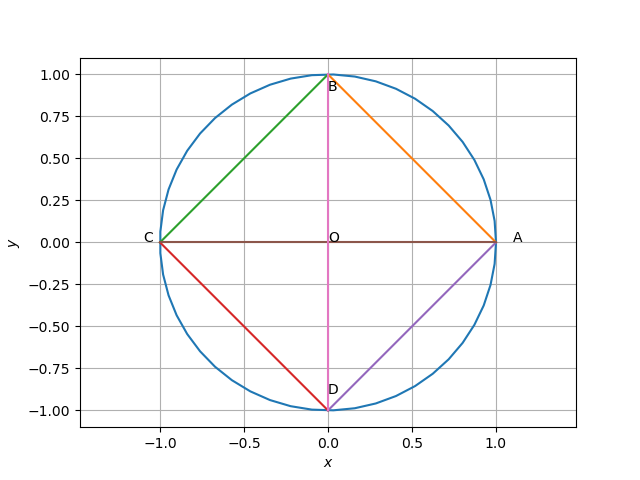
\includegraphics[width=\columnwidth]{chapters/9/10/6/7/figs/circle.png}
    \caption{circle}
    \label{fig:chapters/9/10/6/7/circle}
\end{figure}


\item Two congruent circles intersect each other at points $\vec{A}$ and $\vec{B}$. Through $\vec{A}$ any line segment $\vec{PAQ}$ is drawn so that $\vec{P}$, $\vec{Q}$ lie on the two circles. Prove that $BP = BQ$.
\label{chapters/9/10/6/9}
\\
    \solution 
\iffalse
\documentclass[journal,12pt,twocolumn]{IEEEtran}
\usepackage{setspace}
\usepackage{gensymb}
\singlespacing
\usepackage[cmex10]{amsmath}
\usepackage{amsthm}
\usepackage{mathrsfs}
\usepackage{txfonts}
\usepackage{stfloats}
\usepackage{bm}
\usepackage{cite}
\usepackage{cases}
\usepackage{subfig}
\usepackage{longtable}
\usepackage{multirow}
\usepackage{enumitem}
\usepackage{mathtools}
\usepackage{steinmetz}
\usepackage{tikz}
\usepackage{circuitikz}
\usepackage{verbatim}
\usepackage{tfrupee}
\usepackage[breaklinks=true]{hyperref}
\usepackage{tkz-euclide}
\usetikzlibrary{calc,math}
\usepackage{listings}
    \usepackage{color}                                            %%
    \usepackage{array}                                            %%
    \usepackage{longtable}                                        %%
    \usepackage{calc}                                             %%
    \usepackage{multirow}                                         %%
    \usepackage{hhline}                                           %%
    \usepackage{ifthen}                                           %%
  %optionally (for landscape tables embedded in another document): %%
    \usepackage{lscape}     
\usepackage{multicol}
\usepackage{chngcntr}
\DeclareMathOperator*{\Res}{Res}
\renewcommand\thesection{\arabic{section}}
\renewcommand\thesubsection{\thesection.\arabic{subsection}}
\renewcommand\thesubsubsection{\thesubsection.\arabic{subsubsection}}

\renewcommand\thesectiondis{\arabic{section}}
\renewcommand\thesubsectiondis{\thesectiondis.\arabic{subsection}}
\renewcommand\thesubsubsectiondis{\thesubsectiondis.\arabic{subsubsection}}

% correct bad hyphenation here
\hyphenation{op-tical net-works semi-conduc-tor}
\def\inputGnumericTable{}                                 %%

\lstset{
frame=single, 
breaklines=true,
columns=fullflexible
}

\begin{document}


\newtheorem{theorem}{Theorem}[section]
\newtheorem{problem}{Problem}
\newtheorem{proposition}{Proposition}[section]
\newtheorem{lemma}{Lemma}[section]
\newtheorem{corollary}[theorem]{Corollary}
\newtheorem{example}{Example}[section]
\newtheorem{definition}[problem]{Definition}
\newcommand{\BEQA}{\begin{eqnarray}}
\newcommand{\EEQA}{\end{eqnarray}}
\newcommand{\define}{\stackrel{\triangle}{=}}

\bibliographystyle{IEEEtran}
\providecommand{\mbf}{\mathbf}
\providecommand{\pr}[1]{\ensuremath{\Pr\left(#1\right)}}
\providecommand{\qfunc}[1]{\ensuremath{Q\left(#1\right)}}
\providecommand{\sbrak}[1]{\ensuremath{{}\left[#1\right]}}
\providecommand{\lsbrak}[1]{\ensuremath{{}\left[#1\right.}}
\providecommand{\rsbrak}[1]{\ensuremath{{}\left.#1\right]}}
\providecommand{\brak}[1]{\ensuremath{\left(#1\right)}}
\providecommand{\lbrak}[1]{\ensuremath{\left(#1\right.}}
\providecommand{\rbrak}[1]{\ensuremath{\left.#1\right)}}
\providecommand{\cbrak}[1]{\ensuremath{\left\{#1\right\}}}
\providecommand{\lcbrak}[1]{\ensuremath{\left\{#1\right.}}
\providecommand{\rcbrak}[1]{\ensuremath{\left.#1\right\}}}
\theoremstyle{remark}
\newtheorem{rem}{Remark}
\newcommand{\sgn}{\mathop{\mathrm{sgn}}}
\providecommand{\abs}[1]{\left\vert#1\right\vert}
\providecommand{\res}[1]{\Res\displaylimits_{#1}} 
\providecommand{\norm}[1]{\left\lVert#1\right\rVert}
\providecommand{\mtx}[1]{\mathbf{#1}}
\providecommand{\mean}[1]{E\left[ #1 \right]}
\providecommand{\fourier}{\overset{\mathcal{F}}{ \rightleftharpoons}}
\providecommand{\system}{\overset{\mathcal{H}}{ \longleftrightarrow}}
\newcommand{\solution}{\noindent \textbf{Solution: }}
\newcommand{\cosec}{\,\text{cosec}\,}
\providecommand{\dec}[2]{\ensuremath{\overset{#1}{\underset{#2}{\gtrless}}}}
\newcommand{\myvec}[1]{\ensuremath{\begin{pmatrix}#1\end{pmatrix}}}
\newcommand{\mydet}[1]{\ensuremath{\begin{vmatrix}#1\end{vmatrix}}}
\numberwithin{equation}{subsection}
\makeatletter
\@addtoreset{figure}{problem}
\makeatother

\let\StandardTheFigure\thefigure
\let\vec\mathbf
\renewcommand{\thefigure}{\theproblem}



\def\putbox#1#2#3{\makebox[0in][l]{\makebox[#1][l]{}\raisebox{\baselineskip}[0in][0in]{\raisebox{#2}[0in][0in]{#3}}}}
     \def\rightbox#1{\makebox[0in][r]{#1}}
     \def\centbox#1{\makebox[0in]{#1}}
     \def\topbox#1{\raisebox{-\baselineskip}[0in][0in]{#1}}
     \def\midbox#1{\raisebox{-0.5\baselineskip}[0in][0in]{#1}}

\vspace{3cm}


\title{Assignment 1}
\author{Jaswanth Chowdary Madala}





% make the title area
\maketitle

\newpage

%\tableofcontents

\bigskip

\renewcommand{\thefigure}{\theenumi}
\renewcommand{\thetable}{\theenumi}


\begin{enumerate}

\textbf{Solution:}
\fi
The parameters used in the construction are shown in Table \ref{tab:chapters/9/10/6/9/1}.
Let the equations of these circles be given by
\begin{align}
\norm{\vec{x}}^2 + 2\vec{u_1}^\top\vec{x} + f &= 0 
\label{eq:chapters/9/10/6/9/1}\\
\norm{\vec{x}}^2 + 2\vec{u_2}^\top\vec{x} + f &= 0 
\label{eq:chapters/9/10/6/9/2}\\
\vec{u_1} = -\myvec{2\\0}, \, \vec{u_2} &= -\myvec{-2\\0}\\
f = -4. 
\end{align}
The common chord of the circles is given by
\begin{align}
2\vec{u_1}^\top\vec{x}-2\vec{u_2}^\top\vec{x}+f_1 - f_2 &= 0\\
\implies
\myvec{1&0}\vec{x} &= 0
\label{eq:chapters/9/10/6/9/3}
\end{align}
\eqref{eq:chapters/9/10/6/9/3} can be written in parametric form as
\begin{align}
	\vec{h} &= \myvec{0\\0}, \, \vec{m} = \myvec{0\\1}\\
	\vec{x} &= \vec{h}+ \mu \vec{m}
\label{eq:chapters/9/10/6/9/4}
\end{align} 
The parameter $\mu$ for the points of intersection of the above line with the given conic
		%line \eqref{eq:chapters/9/10/6/9/5} with the conic section \eqref{eq:chapters/9/10/6/9/6}
is given by the equation 
\begin{align}
\mu^2\vec{m}^{\top}\vec{V}\vec{m} + 2 \mu\vec{m}^{\top}\brak{\vec{V}\vec{h}+\vec{u}} + \text{g}\brak{\vec{h}} &=0
\label{eq:chapters/9/10/6/9/7}
\end{align}
Substituting numerical values,
\begin{align}
\vec{V} = \vec{I}, \, \vec{u} &= \myvec{-2\\0}, \, f = -4,\,
\vec{h} = \myvec{0\\0}, \, \vec{m} &= \myvec{0\\1}\\
\end{align}
we obtain 
\begin{align}
\mu^2 - 4 =0
\implies \mu = \pm 2
\end{align}
From \eqref{eq:chapters/9/10/6/9/4}, 
\begin{align}
\vec{A} = \myvec{0\\2},\,
\vec{B} = \myvec{0\\-2} 
\end{align} 
Since 
\begin{align}
\vec{m} = \myvec{2\\1}
\label{eq:chapters/9/10/6/9/8}
\end{align} 
The equation of the line passing through the point $\vec{A}$ with the direction vector \eqref{eq:chapters/9/10/6/9/8} in parametric form is given by,
\begin{align}
\vec{x} = \myvec{0\\2} + \alpha\myvec{2\\1}
\label{eq:chapters/9/10/6/9/9}
\end{align}
Substituing 
\begin{align}
\vec{V} = \vec{I}, \, \vec{u} &= \myvec{-2\\0}, \, f = -4
\vec{h} = \myvec{0\\2}, 
\end{align}
the intersection of the line in 
\ref{eq:chapters/9/10/6/9/9}
with one circle is given by 
\begin{align}
5\alpha^2 - 4 \alpha &=0
\implies \alpha &= 0, \frac{4}{5}
\end{align}
Thus,
\begin{align}
\vec{P} &= \myvec{\frac{8}{5}\\\\ \frac{14}{5}}
\end{align}
Similarly, the intersection with the second circle is given by 
\begin{align}
	5\beta^2 + 12 \beta &=0,\,
\implies \beta = 0, -\frac{12}{5}\\
	\text{and } \vec{Q} &= \myvec{-\frac{24}{5}\\\\-\frac{2}{5}}
\end{align}
Thus, 
\begin{align}
	\norm{\vec{B}-\vec{P}} &=  
\norm{\vec{B}-\vec{Q}} =  \frac{8\sqrt{10}}{5}
\\
\implies 
	BP &= BQ.
\end{align}
See Fig.
\ref{fig:chapters/9/10/6/9/1}.
\begin{table}[h]
\centering
%%%%%%%%%%%%%%%%%%%%%%%%%%%%%%%%%%%%%%%%%%%%%%%%%%%%%%%%%%%%%%%%%%%%%%
%%                                                                  %%
%%  This is a LaTeX2e table fragment exported from Gnumeric.        %%
%%                                                                  %%
%%%%%%%%%%%%%%%%%%%%%%%%%%%%%%%%%%%%%%%%%%%%%%%%%%%%%%%%%%%%%%%%%%%%%%

\begin{center}
\begin{tabular}{|c|c|c|}
\hline
\textbf{Parameter}	&\textbf{Description}& \textbf{Value}\\ \hline
$\vec{C}_1$	&center of circle 1&	$\myvec{-2\\0}$\\ \hline
$r_1$		&radius of circle 1&	$2\sqrt{2}$\\ \hline
$\vec{C}_2$	&center of circle 2&	$\myvec{2\\0}$\\ \hline
$r_2$		&radius of circle 2&	$2\sqrt{2}$\\ \hline
$\vec{m}$	&direction vector of the line passing through $\vec{A}$&	$\myvec{2\\1}$\\ \hline
\end{tabular}
\end{center}

\caption{}
\label{tab:chapters/9/10/6/9/1}
\end{table}
\begin{figure}[ht]
\centering
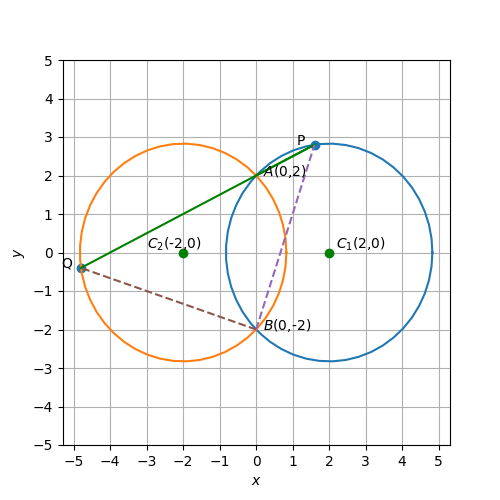
\includegraphics[width = \columnwidth]{chapters/9/10/6/9/figs/fig.png}
\caption{}
\label{fig:chapters/9/10/6/9/1}
\end{figure}

\item In any $\triangle ABC$, if the angle bisector of $\angle A$ and 
    perpendicular bisector of $BC$ intersect, prove that they intersect on 
    the circumcircle of $\triangle ABC$.
\\
    \solution 
\label{chapters/9/10/6/10}
\iffalse
\documentclass[journal,12pt,twocolumn]{IEEEtran}
\usepackage{setspace}
\usepackage{gensymb}
\singlespacing
\usepackage[cmex10]{amsmath}
\usepackage{amsthm}
\usepackage{mathrsfs}
\usepackage{txfonts}
\usepackage{stfloats}
\usepackage{bm}
\usepackage{cite}
\usepackage{cases}
\usepackage{subfig}
\usepackage{longtable}
\usepackage{multirow}
\usepackage{enumitem}
\usepackage{mathtools}
\usepackage{tikz}
\usepackage{circuitikz}
\usepackage{verbatim}
\usepackage[breaklinks=true]{hyperref}
\usepackage{tkz-euclide} % loads  TikZ and tkz-base
\usepackage{listings}
\usepackage{color}    
\usepackage{array}    
\usepackage{longtable}
\usepackage{calc}     
\usepackage{multirow} 
\usepackage{hhline}   
\usepackage{ifthen}   
\usepackage{lscape}     
\usepackage{chngcntr}
\DeclareMathOperator*{\Res}{Res}
\renewcommand\thesection{\arabic{section}}
\renewcommand\thesubsection{\thesection.\arabic{subsection}}
\renewcommand\thesubsubsection{\thesubsection.\arabic{subsubsection}}

\renewcommand\thesectiondis{\arabic{section}}
\renewcommand\thesubsectiondis{\thesectiondis.\arabic{subsection}}
\renewcommand\thesubsubsectiondis{\thesubsectiondis.\arabic{subsubsection}}
\renewcommand\thetable{\arabic{table}}
% correct bad hyphenation here
\hyphenation{op-tical net-works semi-conduc-tor}
\def\inputGnumericTable{}                                 %%

\lstset{
%language=C,
frame=single, 
breaklines=true,
columns=fullflexible
}
%\lstset{
%language=tex,
%frame=single, 
%breaklines=true
%}

\begin{document}
\newtheorem{theorem}{Theorem}[section]
\newtheorem{problem}{Problem}
\newtheorem{proposition}{Proposition}[section]
\newtheorem{lemma}{Lemma}[section]
\newtheorem{corollary}[theorem]{Corollary}
\newtheorem{example}{Example}[section]
\newtheorem{definition}[problem]{Definition}
\newcommand{\BEQA}{\begin{eqnarray}}
\newcommand{\EEQA}{\end{eqnarray}}
\newcommand{\define}{\stackrel{\triangle}{=}}
\bibliographystyle{IEEEtran}
\providecommand{\mbf}{\mathbf}
\providecommand{\pr}[1]{\ensuremath{\Pr\left(#1\right)}}
\providecommand{\qfunc}[1]{\ensuremath{Q\left(#1\right)}}
\providecommand{\sbrak}[1]{\ensuremath{{}\left[#1\right]}}
\providecommand{\lsbrak}[1]{\ensuremath{{}\left[#1\right.}}
\providecommand{\rsbrak}[1]{\ensuremath{{}\left.#1\right]}}
\providecommand{\brak}[1]{\ensuremath{\left(#1\right)}}
\providecommand{\lbrak}[1]{\ensuremath{\left(#1\right.}}
\providecommand{\rbrak}[1]{\ensuremath{\left.#1\right)}}
\providecommand{\cbrak}[1]{\ensuremath{\left\{#1\right\}}}
\providecommand{\lcbrak}[1]{\ensuremath{\left\{#1\right.}}
\providecommand{\rcbrak}[1]{\ensuremath{\left.#1\right\}}}
\theoremstyle{remark}
\newtheorem{rem}{Remark}
\newcommand{\sgn}{\mathop{\mathrm{sgn}}}
\providecommand{\abs}[1]{\left\vert#1\right\vert}
\providecommand{\res}[1]{\Res\displaylimits_{#1}} 
\providecommand{\norm}[1]{\left\lVert#1\right\rVert}
\providecommand{\mtx}[1]{\mathbf{#1}}
\providecommand{\mean}[1]{E\left[ #1 \right]}
\providecommand{\fourier}{\overset{\mathcal{F}}{ \rightleftharpoons}}
\providecommand{\system}[1]{\overset{\mathcal{#1}}{ \longleftrightarrow}}
\newcommand{\solution}{\noindent \textbf{Solution: }}
\newcommand{\cosec}{\,\text{cosec}\,}
\providecommand{\dec}[2]{\ensuremath{\overset{#1}{\underset{#2}{\gtrless}}}}
\newcommand{\myvec}[1]{\ensuremath{\begin{pmatrix}#1\end{pmatrix}}}
\newcommand{\mydet}[1]{\ensuremath{\begin{vmatrix}#1\end{vmatrix}}}
\let\vec\mathbf
\def\putbox#1#2#3{\makebox[0in][l]{\makebox[#1][l]{}\raisebox{\baselineskip}[0in][0in]{\raisebox{#2}[0in][0in]{#3}}}}
     \def\rightbox#1{\makebox[0in][r]{#1}}
     \def\centbox#1{\makebox[0in]{#1}}
     \def\topbox#1{\raisebox{-\baselineskip}[0in][0in]{#1}}
     \def\midbox#1{\raisebox{-0.5\baselineskip}[0in][0in]{#1}}

\vspace{3cm}
\title{Circle Assignment}
\author{Gautam Singh}
\maketitle
\bigskip

\begin{abstract}
    This document contains the solution to Question 10 of 
    Exercise 6 in Chapter 10 of the class 9 NCERT textbook.
\end{abstract}

\begin{enumerate}
    
    \fi
		Let the position vectors of the points be
    \begin{align}
        \vec{A} = \myvec{1\\0},\ \vec{B} = \myvec{\cos\beta\\\sin\beta},\ \vec{C} = \myvec{\cos\gamma\\\sin\gamma}
        \label{eq:chapters/9/10/6/10/pts}
    \end{align}

    Then, the equation of the perpendicular bisector of $BC$ is given by
    \begin{align}
        \norm{\vec{x}-\vec{B}}^2&=\norm{\vec{x}-\vec{C}}^2 \\
        \implies \brak{\vec{B}-\vec{C}}^\top\vec{x} &= 0
        \label{eq:chapters/9/10/6/10/perp-bisect}
    \end{align}
    and the equation of the angle bisector of $\angle A$ is given by
    \begin{align}
        &\frac{\brak{\vec{B}-\vec{A}}^\top\brak{\vec{x}-\vec{A}}}{\norm{\vec{B}-\vec{A}}} = \frac{\brak{\vec{C}-\vec{A}}^\top\brak{\vec{x}-\vec{A}}}{\norm{\vec{C}-\vec{A}}} \\
        &\brak{\frac{\vec{B}-\vec{A}}{\norm{\vec{B}-\vec{A}}}-\frac{\vec{C}-\vec{A}}{\norm{\vec{C}-\vec{A}}}}^\top\brak{\vec{x}-\vec{A}} = 0
        \label{eq:chapters/9/10/6/10/angle-bisect}
    \end{align}
    Note that from \eqref{eq:chapters/9/10/6/10/pts},
    \begin{align}
        \frac{\vec{B}-\vec{A}}{\norm{\vec{B}-\vec{A}}} &= \frac{1}{\sqrt{2\brak{1-\cos\beta}}}\myvec{\cos\beta-1\\\sin\beta} \\
                                                       &= \myvec{-\sin\frac{\beta}{2}\\\cos\frac{\beta}{2}}
                                                       \label{eq:chapters/9/10/6/10/unit-vec}
    \end{align}
    Therefore, using \eqref{eq:chapters/9/10/6/10/pts} in \eqref{eq:chapters/9/10/6/10/perp-bisect} and
    \eqref{eq:chapters/9/10/6/10/unit-vec} in \eqref{eq:chapters/9/10/6/10/angle-bisect},
    \begin{align}
        \myvec{\cos\beta-\cos\gamma\\\sin\beta-\sin\gamma}^\top\vec{x} &= 0 \label{eq:chapters/9/10/6/10/e1} \\
        \myvec{\sin\frac{\gamma}{2}-\sin\frac{\beta}{2}\\\cos\frac{\beta}{2}-\cos\frac{\gamma}{2}}^\top\vec{x} &= \sin\frac{\gamma}{2}-\sin\frac{\beta}{2} \label{eq:chapters/9/10/6/10/e2}
    \end{align}
    Using \eqref{eq:chapters/9/10/6/10/e1} and \eqref{eq:chapters/9/10/6/10/e2}, we form the matrix equation
    \begin{align}
        \myvec{\cos\beta-\cos\gamma&\sin\beta-\sin\gamma\\\sin\frac{\gamma}{2}-\sin\frac{\beta}{2}&\cos\frac{\beta}{2}-\cos\frac{\gamma}{2}}\vec{x} \nonumber \\
        = \myvec{0\\\sin\frac{\gamma}{2}-\sin\frac{\beta}{2}}
        \label{eq:chapters/9/10/6/10/mtx-eqn}
    \end{align}
    Solving \eqref{eq:chapters/9/10/6/10/mtx-eqn} using the augmented matrix, and letting 
    $\theta \triangleq \frac{\beta+\gamma}{2}$,
    \begin{align}
        &\myvec{\cos\beta-\cos\gamma&\sin\beta-\sin\gamma&0\\\sin\frac{\gamma}{2}-\sin\frac{\beta}{2}&\cos\frac{\beta}{2}-\cos\frac{\gamma}{2}&\sin\frac{\gamma}{2}-\sin\frac{\beta}{2}} \\
        &\xleftrightarrow[]{\substack{R_1\leftarrow\frac{R_1}{\cos\beta-\cos\gamma}\\R_2\leftarrow\frac{R_2}{\sin\frac{\gamma}{2}-\sin\frac{\beta}{2}}}}\myvec{1&-\cot\theta&0\\1&\tan\frac{\theta}{2}&1} \\
        &\xleftrightarrow[]{R_2\leftarrow R_2-R_1}\myvec{1&-\cot\theta&0\\0&\tan\frac{\theta}{2}+\cot\theta&1} \\
        &= \myvec{1&-\cot\theta&0\\0&\csc\theta&1} \\
        &\xleftrightarrow[]{R_1\leftarrow R_1 + R_2\cos\theta}\myvec{1&0&\cos\theta\\0&\csc\theta&1} \\
        &\xleftrightarrow[]{R_2\leftarrow R_2\sin\theta}\myvec{1&0&\cos\theta\\0&1&\sin\theta}
        \label{eq:chapters/9/10/6/10/aug-mtx}
    \end{align}
    Thus, the intersection of the lines in \eqref{eq:chapters/9/10/6/10/e1} and \eqref{eq:chapters/9/10/6/10/e2} is
    \begin{align}
        \vec{D} \triangleq \myvec{\cos\frac{\beta+\gamma}{2}\\\sin\frac{\beta+\gamma}{2}}
        \label{eq:chapters/9/10/6/10/intersect-pt}
    \end{align}
    Hence, it is clear from \eqref{eq:chapters/9/10/6/10/intersect-pt} that $\vec{D}$ lies on the 
    circumcircle of $\triangle ABC$, as required.

    The situation is illustrated in Fig. \ref{fig:chapters/9/10/6/10/bisector}. The parameters
    used in the construction are shown in Table \ref{tab:chapters/9/10/6/10/param}.
    \begin{table}[!ht]
        \centering
        %%%%%%%%%%%%%%%%%%%%%%%%%%%%%%%%%%%%%%%%%%%%%%%%%%%%%%%%%%%%%%%%%%%%%%
%%                                                                  %%
%%  This is the header of a LaTeX2e file exported from Gnumeric.    %%
%%                                                                  %%
%%  This file can be compiled as it stands or included in another   %%
%%  LaTeX document. The table is based on the longtable package so  %%
%%  the longtable options (headers, footers...) can be set in the   %%
%%  preamble section below (see PRAMBLE).                           %%
%%                                                                  %%
%%  To include the file in another, the following two lines must be %%
%%  in the including file:                                          %%
%%        \def\inputGnumericTable{}                                 %%
%%  at the beginning of the file and:                               %%
%%        \input{name-of-this-file.tex}                             %%
%%  where the table is to be placed. Note also that the including   %%
%%  file must use the following packages for the table to be        %%
%%  rendered correctly:                                             %%
%%    \usepackage[latin1]{inputenc}                                 %%
%%    \usepackage{color}                                            %%
%%    \usepackage{array}                                            %%
%%    \usepackage{longtable}                                        %%
%%    \usepackage{calc}                                             %%
%%    \usepackage{multirow}                                         %%
%%    \usepackage{hhline}                                           %%
%%    \usepackage{ifthen}                                           %%
%%  optionally (for landscape tables embedded in another document): %%
%%    \usepackage{lscape}                                           %%
%%                                                                  %%
%%%%%%%%%%%%%%%%%%%%%%%%%%%%%%%%%%%%%%%%%%%%%%%%%%%%%%%%%%%%%%%%%%%%%%



%%  This section checks if we are begin input into another file or  %%
%%  the file will be compiled alone. First use a macro taken from   %%
%%  the TeXbook ex 7.7 (suggestion of Han-Wen Nienhuys).            %%
\def\ifundefined#1{\expandafter\ifx\csname#1\endcsname\relax}


%%  Check for the \def token for inputed files. If it is not        %%
%%  defined, the file will be processed as a standalone and the     %%
%%  preamble will be used.                                          %%
\ifundefined{inputGnumericTable}

%%  We must be able to close or not the document at the end.        %%
	\def\gnumericTableEnd{\end{document}}


%%%%%%%%%%%%%%%%%%%%%%%%%%%%%%%%%%%%%%%%%%%%%%%%%%%%%%%%%%%%%%%%%%%%%%
%%                                                                  %%
%%  This is the PREAMBLE. Change these values to get the right      %%
%%  paper size and other niceties.                                  %%
%%                                                                  %%
%%%%%%%%%%%%%%%%%%%%%%%%%%%%%%%%%%%%%%%%%%%%%%%%%%%%%%%%%%%%%%%%%%%%%%

	\documentclass[12pt%
			  %,landscape%
                    ]{report}
       \usepackage[latin1]{inputenc}
       \usepackage{fullpage}
       \usepackage{color}
       \usepackage{array}
       \usepackage{longtable}
       \usepackage{calc}
       \usepackage{multirow}
       \usepackage{hhline}
       \usepackage{ifthen}

	\begin{document}


%%  End of the preamble for the standalone. The next section is for %%
%%  documents which are included into other LaTeX2e files.          %%
\else

%%  We are not a stand alone document. For a regular table, we will %%
%%  have no preamble and only define the closing to mean nothing.   %%
    \def\gnumericTableEnd{}

%%  If we want landscape mode in an embedded document, comment out  %%
%%  the line above and uncomment the two below. The table will      %%
%%  begin on a new page and run in landscape mode.                  %%
%       \def\gnumericTableEnd{\end{landscape}}
%       \begin{landscape}


%%  End of the else clause for this file being \input.              %%
\fi

%%%%%%%%%%%%%%%%%%%%%%%%%%%%%%%%%%%%%%%%%%%%%%%%%%%%%%%%%%%%%%%%%%%%%%
%%                                                                  %%
%%  The rest is the gnumeric table, except for the closing          %%
%%  statement. Changes below will alter the table's appearance.     %%
%%                                                                  %%
%%%%%%%%%%%%%%%%%%%%%%%%%%%%%%%%%%%%%%%%%%%%%%%%%%%%%%%%%%%%%%%%%%%%%%

\providecommand{\gnumericmathit}[1]{#1} 
%%  Uncomment the next line if you would like your numbers to be in %%
%%  italics if they are italizised in the gnumeric table.           %%
%\renewcommand{\gnumericmathit}[1]{\mathit{#1}}
\providecommand{\gnumericPB}[1]%
{\let\gnumericTemp=\\#1\let\\=\gnumericTemp\hspace{0pt}}
 \ifundefined{gnumericTableWidthDefined}
        \newlength{\gnumericTableWidth}
        \newlength{\gnumericTableWidthComplete}
        \newlength{\gnumericMultiRowLength}
        \global\def\gnumericTableWidthDefined{}
 \fi
%% The following setting protects this code from babel shorthands.  %%
 \ifthenelse{\isundefined{\languageshorthands}}{}{\languageshorthands{english}}
%%  The default table format retains the relative column widths of  %%
%%  gnumeric. They can easily be changed to c, r or l. In that case %%
%%  you may want to comment out the next line and uncomment the one %%
%%  thereafter                                                      %%
\providecommand\gnumbox{\makebox[0pt]}
%%\providecommand\gnumbox[1][]{\makebox}

%% to adjust positions in multirow situations                       %%
\setlength{\bigstrutjot}{\jot}
\setlength{\extrarowheight}{\doublerulesep}

%%  The \setlongtables command keeps column widths the same across  %%
%%  pages. Simply comment out next line for varying column widths.  %%
\setlongtables

\setlength\gnumericTableWidth{%
	60pt+%
	67pt+%
0pt}
\def\gumericNumCols{2}
\setlength\gnumericTableWidthComplete{\gnumericTableWidth+%
         \tabcolsep*\gumericNumCols*2+\arrayrulewidth*\gumericNumCols}
\ifthenelse{\lengthtest{\gnumericTableWidthComplete > \linewidth}}%
         {\def\gnumericScale{1*\ratio{\linewidth-%
                        \tabcolsep*\gumericNumCols*2-%
                        \arrayrulewidth*\gumericNumCols}%
{\gnumericTableWidth}}}%
{\def\gnumericScale{1}}

%%%%%%%%%%%%%%%%%%%%%%%%%%%%%%%%%%%%%%%%%%%%%%%%%%%%%%%%%%%%%%%%%%%%%%
%%                                                                  %%
%% The following are the widths of the various columns. We are      %%
%% defining them here because then they are easier to change.       %%
%% Depending on the cell formats we may use them more than once.    %%
%%                                                                  %%
%%%%%%%%%%%%%%%%%%%%%%%%%%%%%%%%%%%%%%%%%%%%%%%%%%%%%%%%%%%%%%%%%%%%%%

\ifthenelse{\isundefined{\gnumericColA}}{\newlength{\gnumericColA}}{}\settowidth{\gnumericColA}{\begin{tabular}{@{}p{60pt*\gnumericScale}@{}}x\end{tabular}}
\ifthenelse{\isundefined{\gnumericColB}}{\newlength{\gnumericColB}}{}\settowidth{\gnumericColB}{\begin{tabular}{@{}p{67pt*\gnumericScale}@{}}x\end{tabular}}

\begin{tabular}[c]{%
	b{\gnumericColA}%
	b{\gnumericColB}%
	}

%%%%%%%%%%%%%%%%%%%%%%%%%%%%%%%%%%%%%%%%%%%%%%%%%%%%%%%%%%%%%%%%%%%%%%
%%  The longtable options. (Caption, headers... see Goosens, p.124) %%
%	\caption{The Table Caption.}             \\	%
% \hline	% Across the top of the table.
%%  The rest of these options are table rows which are placed on    %%
%%  the first, last or every page. Use \multicolumn if you want.    %%

%%  Header for the first page.                                      %%
%	\multicolumn{2}{c}{The First Header} \\ \hline 
%	\multicolumn{1}{c}{colTag}	%Column 1
%	&\multicolumn{1}{c}{colTag}	\\ \hline %Last column
%	\endfirsthead

%%  The running header definition.                                  %%
%	\hline
%	\multicolumn{2}{l}{\ldots\small\slshape continued} \\ \hline
%	\multicolumn{1}{c}{colTag}	%Column 1
%	&\multicolumn{1}{c}{colTag}	\\ \hline %Last column
%	\endhead

%%  The running footer definition.                                  %%
%	\hline
%	\multicolumn{2}{r}{\small\slshape continued\ldots} \\
%	\endfoot

%%  The ending footer definition.                                   %%
%	\multicolumn{2}{c}{That's all folks} \\ \hline 
%	\endlastfoot
%%%%%%%%%%%%%%%%%%%%%%%%%%%%%%%%%%%%%%%%%%%%%%%%%%%%%%%%%%%%%%%%%%%%%%

\hhline{|-|-}
	 \multicolumn{1}{|p{\gnumericColA}|}%
	{\gnumericPB{\centering}\gnumbox{\textbf{Parameter}}}
	&\multicolumn{1}{p{\gnumericColB}|}%
	{\gnumericPB{\centering}\gnumbox{\textbf{Value}}}
\\
\hhline{|--|}
	 \multicolumn{1}{|p{\gnumericColA}|}%
	{\gnumericPB{\centering}\gnumbox{$r$}}
	&\multicolumn{1}{p{\gnumericColB}|}%
	{\gnumericPB{\centering}\gnumbox{1}}
\\
\hhline{|--|}
	 \multicolumn{1}{|p{\gnumericColA}|}%
	{\gnumericPB{\centering}\gnumbox{$\beta$}}
	&\multicolumn{1}{p{\gnumericColB}|}%
    {\gnumericPB{\centering}\gnumbox{100$^{\circ}$}}
\\
\hhline{|--|}
	 \multicolumn{1}{|p{\gnumericColA}|}%
	{\gnumericPB{\centering}\gnumbox{$\gamma$}}
	&\multicolumn{1}{p{\gnumericColB}|}%
    {\gnumericPB{\centering}\gnumbox{200$^{\circ}$}}
\\
\hhline{|-|-|}
\end{tabular}

\ifthenelse{\isundefined{\languageshorthands}}{}{\languageshorthands{\languagename}}
\gnumericTableEnd

        \caption{Parameters used in the construction of Fig. \ref{fig:chapters/9/10/6/10/bisector}.}
        \label{tab:chapters/9/10/6/10/param}
    \end{table}
    \begin{figure}[!ht]
        \centering
        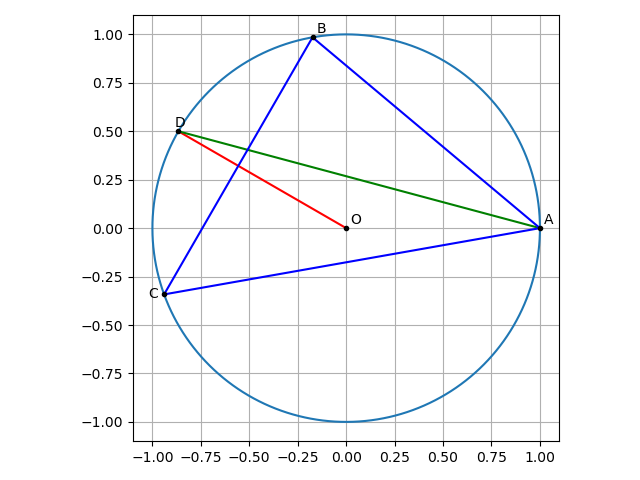
\includegraphics[width=\columnwidth]{chapters/9/10/6/10/figs/bisector.png}
        \caption{The bisector of $\angle A$ and of $BC$ meet on the circumcircle at $D$.}
        \label{fig:chapters/9/10/6/10/bisector}
    \end{figure}



\end{enumerate}
